\documentclass{coursbook}

\begin{document}
    \begin{titlepage} \centering
        \title{Cours de Spécialité Mathématique}
        \subtitle{Terminale, Année 2021}
        \author{\and Diego Van Overberghe}
    \end{titlepage}

    \maketitle
    \tableofcontents

    \chapter{Suites : La Démonstration par Récurrence}

    % \setlength{\baselineskip}{1.5em}
    \begin{Gpartie}{Exemple}
        On considère la suite $\left(u_n\right)$, définie pour tout $n\in\mathbb{N}$, par $u_n=4^n-1$ :
            \[\left(u_n\right)=\big\{~0~;~3~;~15~;63~;~255~;\dotsc~\big\}\]
        On remarque que tous ces nombres sont des multiples de 3. On se demande si $\forall n\in\mathbb{N},~4^n-1$ est un multiple de 3.
    \end{Gpartie}
    \begin{Gpartie}{Axiome de Récurrence}
        Soit $\Pde(n)$, une propriété dépendante de l'entier naturel $n$.\\
        Si :
        \[\begin{cases}
            \Pde(0)\text{ est vraie (Initialisation)} \\ \forall k\in\mathbb{N},~\Pde(k)\text{ vraie}\implies\Pde(k+1)\text{ vraie (hérédité)}
        \end{cases}\]

        Alors : $P(n)$ est vraie pour tout entier naturel. \\[4ex]
        Reprenons notre exemple. La propriété : \og $4^n-1$ est un multiple de 3 \fg{}, est vraie pour $n=0$. La propriété est donc initialisée.
        
        Hérédité : Supposons que la propriété est vraie à un certain rang $k$, (fixe). C'est~l'hypothèse de la récurrence, et montrons qu'alors, elle est vraie au rang $k+1$.
        
        L'Hypothèse de récurrence est donc : \og $4^n-1$ est un multiple de 3 \fg{}. C'est-à-dire qu'il existe un entier $p$ tel que $\quad4^n-1=3p\quad$ et donc $\quad4^n=3p+1$.
        \[\begin{aligned}[t]
            4^{k+1}-1&=4\times 4^k-1 &\\
            &= 4\times\left(3p+1\right)-1 \quad \text{(Hypothèse de récurrence)} &\\
            &=12p+4-1 &\\
            &=12p+3 &\\
            &=3\left(4p+1\right) \quad \text{(Il s'agit bien d'un multiple de 3)}
        \end{aligned}\]
        Donc, la propriété est héréditaire.

        On a démontré par récurrence que $\forall n\in\mathbb{N},4^n-1$ est un multiple de 3.
    \end{Gpartie}



    \chapter{Continuité des Fonctions d'une Variable~Réelle}

    \begin{Gpartie}{Définition}
        Soit $f$, définie sur un intervalle $I$, et soit $a$, un réel de $I$.
        La fonction $f$ est \emph{continue} si et seulement si : \[\boxed{\lim_{x \to a} f(x)=f(a)}\]
        $f$ est continue sur l'intervalle $I$, si et seulement si, quel que soit le réel $x\in I$, $f$ est continue en $x$.

        H.P.: $\quad\forall\epsilon >0,~\exists\alpha >0,~\forall x\in\big]a-\alpha~;a+\alpha\big[,~f(x)\in\big]f(a)-\epsilon~;f(a)+\epsilon\big[$
        \begin{Spartie}{Exemple}
            La fonction inverse est continue sur $\big]-\infty\,~;~0\,\big[$, et sur $\big]\,0\,~;~+\infty\,\big[$.

            La fonction \og Partie Entière \fg{} est définie sur $\mathbb{R}$, mais pas continue sur $\mathbb{R}$.
            \begin{center}\begin{tikzpicture}[scale=0.7]
                \begin{axis}[
                    xmin=-0.5,  xmax=3.5,
                    ymin=-0.5,  ymax=3.5,
                ]
                    \addplot[color=blue, very thick, jump mark left, samples=5, mark=*, domain=0:4]{floor(x)};
                \end{axis}
            \end{tikzpicture}\end{center}
            \parbox{\linewidth}{\captionof{figure}{\centering Représentation Graphique de la Fonction \og Partie Entière \fg{}, continue sur $\big[n\,~;~n+1\,\big[$ avec $n\in\mathbb{Z}$.}}
            \begin{center}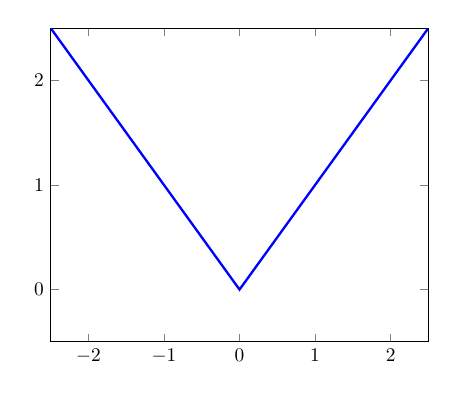
\begin{tikzpicture}[scale=0.7]
                \begin{axis}[
                    xmin=-2.5,  xmax=2.5,
                    ymin=-0.5,  ymax=2.5,
                ]
                    \addplot[color=blue, very thick]{abs(x)};
                \end{axis}
            \end{tikzpicture}\end{center}
            \parbox{\linewidth}{\captionof{figure}{Représentation Graphique de la Fonction Absolue, continue sur $\mathbb{R}$}}
        \end{Spartie}
        \begin{Spartie}{Propriété}
            La somme, le produit et la composée de deux fonctions continues est continue. \\
            L'inverse d'une fonction continue est continue sur tout intervalle où elle ne s'annule pas.
            \[f : x\mapsto x^2\quad\text{continue}\] \[g : x\mapsto\dfrac{1}{x^2}\quad\text{Définie sur }\mathbb{R}^*\text{, continue sur }\big]-\infty\,~;~0\,\big[\text{ et }\big]\,0\,~;~+\infty\,\big]\]
        \end{Spartie}
    \end{Gpartie}

    \hspace{4ex}

    \begin{Gpartie}{Théorème des Valeurs Intermédiaires}
        \begin{Spartie}{Théorème}
            Si une fonction $f$ est continue sur un intervalle $\big[a\,~;~b\,\big]$ alors, pour tout réel $k\in\Big[\mathrm{min}\,\big(f(a)\,~;~f(b)\,\big)\,~;~\mathrm{max}\,\big(f(a)\,~;~f(b)\,\big)\Big]$, il existe \emph{au moins} un réel $c\in\big[a\,~;~b\,\big]$, tel~que $f(c)=k$.

            C'est-à-dire, pour tout réel $k$, compris entre $f(a)$ et $f(b)$, il existe un réel $c\in\big[a\,~;~b\,\big]$, tel que $f(c)=k$.
            \begin{center}
                \begin{tikzpicture}[
                    scale=1.5,
                    % dot/.style={
                    %     draw=black,
                    %     fill=darkgray,
                    %     circle,
                    %     minimum size=2pt,
                    %     inner sep=0pt,
                    %     solid,
                    % },
                ]
                    \begin{axis}[
                        xmin=-5,    xmax=5,
                        ymin=-1,    ymax=5,
                        xtick=\empty,
                        ytick=\empty,
                        domain=-4.9:2.85
                    ]
                        \addplot[color=blue, very thick, samples=50, name path=func]{0.1*x^3+0.3*x^2-0.5*x+1} node[below right]{$\mathcal{C}_f$};
                        \draw[dashed, red, thick]
                            ( -3.6,2 ) -- (-1.4,2) -- (2,2) node [dot, label={[label distance=-2pt]0:$k$}] {}
                            ( -3.6,2 ) node [dot] {} -- (-3.6,0) node [label={[label distance=-6pt]270:$c_1$}] {}
                            ( -1.4,2 ) node [dot] {} -- (-1.4,0) node [label={[label distance=-6pt]270:$c_2$}] {}
                            ( 2,2 ) node [dot] {} -- (2,0) node [label={[label distance=-6pt]270:$c_3$}] {};

                        \draw[dashed, black, thick]
                            (0,4) node [label=left:$f(b)$] {} -- (2.75,4) node [dot] {} -- (2.75,0) node [label=below:$b$] {}
                            (-4.75,0) node [label=above:$a$] {} -- (-4.75,-0.6) node [dot] {} -- (0,-0.6) node [label=right:$f(a)$] {};
                    \end{axis}
                \end{tikzpicture}
                \parbox{\linewidth}{\captionof{figure}{Présentation du Théorème des Valeurs Intermédiaires}}
            \end{center}
            Pour tout $k$ appartenant à $\big[f(b)\,~;~f(a)\,\big]$, il existe au moins un réel $c\in\big[a\,~;~b\,\big]$, tel que $f(c)=k$.
        \end{Spartie}
        \pagebreak
        \begin{Spartie}{Corollaire}
            Si une fonction $f$ est \textit{continue} et \textit{strictement monotone} sur un intervalle $\big[a\,~;~b\,\big]$, alors, pour tout $k\in\Big[\mathrm{min}\,\big(f(a)\,~;~f(b)\,\big)\,~;~\mathrm{max}\,\big(f(a)\,~;~f(b)\,\big)\Big]$, il existe un \textit{unique} réel $c\in\big[a\,~;~b\,\big]$, tel que $f(c)=k$. 
            \begin{center}
                \begin{tikzpicture}[scale=1.5]
                    \begin{axis}[
                        xmin=-0.5,  xmax=1.5,
                        ymin=-0.5,  ymax=2.5,
                        xtick=\empty,
                        ytick=\empty,
                        domain=-0.25:1.05
                    ]
                        \addplot[color=blue, very thick, samples=20]{x^3+x};

                        \draw[dashed, red, thick]
                            (0,1.05) node [label={[label distance=-2pt]180:$k$}] {} -- (0.7,1.05) node [dot] {} -- (0.7,0) node [label={[label distance=-2pt]270:$c$}] {};

                        \draw[dashed, black, thick]
                            (0,0.21) node [label={[label distance=-2pt]180:$f(a)$}] {} -- (0.2,0.21) node [dot] {} -- (0.21,0) node [label={[label distance=-2pt]270:$a$}] {}
                            (0,2) node [label={[label distance=-2pt]180:$f(b)$}] {} -- (1,2) node [dot] {} -- (1,0) node [label={[label distance=-4.5pt]270:$b$}] {};
                    \end{axis}
                \end{tikzpicture}
                \parbox{\linewidth}{\captionof{figure}{\centering Illustration du Corollaire du Théorème \linebreak des Valeurs Intermédiaires}}
            \end{center}
            \begin{SSpartie}{Cas Particulier}
                Si une fonction $f$ est continue sur un intervalle $\big[a\,~;~b\,\big]$, et si $f(a)$ et $f(b)$ sont de signes contraires, il existe au moins une solution à $f(x)=0$, sur $\big[a\,~;~b\,\big]$.
            \end{SSpartie}
        \end{Spartie}
    \end{Gpartie}






    \chapter{Dénombrement et Combinatoire}

    \begin{Gpartie}{Parties d'un Ensemble}
        \begin{Spartie}{Définition}
            $E$ étant un ensemble, la notation $\subset$ signifie \og inclus dans \fg{}.
            \[A\subset E\]
            C'est-à-dire que tout élément de $A$ appartient à $E$. \\
            On dit alors que $A$ est une partie, ou sous-ensemble de $E$. \\
            L'Ensemble vide, noté $\varnothing$ est une \emph{partie} de tout ensemble. \\
            L'Ensemble des parties de $E$ est noté $\mathcal{P}(E)$.
            \begin{SSpartie}{Exemple}
                Si $E=\big\{\,x~;\,y~\big\}$ est un ensemble de deux éléments :
                \[\mathcal{P}(E)=\Big\{\,\varnothing~,\,\big\{\,x~\big\}~,\,\big\{\,y~\big\}~,\,\big\{\,x~;\,y~\big\}~\Big\}\]
            \end{SSpartie}
        \end{Spartie}
        \begin{Spartie}{Définition}
            Un ensemble fini est un ensemble dont le nombre d'éléments est fini.
        \end{Spartie}
        \begin{Spartie}{Définition}
            On appelle cardinal, noté \og Card \fg{}, le nombre d'éléments d'un ensemble fini d'une partie (ou sous-ensemble).
            \begin{SSpartie}{Exemple}
                Si un ensemble $E$ possède $n$ éléments, alors on peut noter $\mathrm{Card}\,(E)=n$. \\
                Pour toute partie $A\subset E$, $\mathrm{Card}\,(A)\leq\mathrm{Card}\,(E)$.
            \end{SSpartie}
        \end{Spartie}
        \begin{Spartie}{Propriété (Principe Additif)}
            Si $A$ et $B$ sont deux parties quelconques d'un ensemble fini $E$, alors :
            \[\mathrm{Card}\,(A\cup B)=\mathrm{Card}\,(A)+\mathrm{Card}\,(B)-\mathrm{Card}\,(A\cap B)\]
            De plus, si $A_1~,~A_2~,\dotsc,~A_p$ sont $p$ parties \emph{deux à deux disjointes} d'un ensemble~fini,~alors~:
            \[\mathrm{Card}\,\left(A_1\cup A_2\cup\dotsb\cup A_p\right)=\mathrm{Card}\,(A_1)+\mathrm{Card}\,(A_2)+\dotsb+\mathrm{Card}\,\left(A_p\right)\]
        \end{Spartie}
        \begin{Spartie}{Propriété}
            Soit $n\in\mathbb{N}$, et $E$ un ensemble tel que $\mathrm{Card}\,(E)=n$. Alors, $E$ possède $2^n$ parties. Autrement dit :
            \[\mathrm{Card}\,\big(\mathcal{P}(E)\big)=2^n\]
            \begin{SSpartie}{Démonstration par Récurrence}
                \begin{SSSpartie}{Initialisation}
                    Pour $n=0$, $E=\varnothing$, donc la seule partie de $E$ est $\big\{\varnothing\big\}$ et $1=2^0$.
                \end{SSSpartie}
                \begin{SSSpartie}{Hérédité}
                    Supposons que tout ensemble à $k$ éléments, où $k$ est un certain entier naturel, admet $2^k$ parties.

                    Alors, soit $E$, un ensemble à $k+1$ éléments.

                    Soit $x$, un élément de $E$.

                    Alors, il y a deux familles de parties de $E$, celles qui contiennent $x$ et celles qui ne le contiennent pas.

                    Or $E\setminus\big\{x\big\}$ est un ensemble à $k$ éléments, il y a donc $2^k$ parties de $E$ qui ne contiennent pas $x$.

                    En adjoignant $x$ à toutes ces parties, on obtient toutes les parties qui contiennent $x$, donc il y en a également $2^k$.
                    
                    Ainsi, le nombre de parties de $E$ est de $2^k+2^k=2^{k+1}$.$\quad\square$
                \end{SSSpartie}
            \end{SSpartie}
        \end{Spartie}
    \end{Gpartie}
    \begin{Gpartie}{Produit Cartésien d'Ensembles}
        \begin{Spartie}{Définition}
            \begin{itemize}
                \item $E$ et $F$ étant deux ensembles, le \emph{produit cartésien} $E\times F$ est l'ensemble de couples $(\,a~;\,b~)$, où $a\in E$ et $b\in F$.
                \item $E$, $F$ et $G$ étant trois ensembles, le \emph{produit cartésien} $E\times F\times G$ est l'ensemble des triplets $(\,a~;\,b~;\,c~)$ où $a\in E$, $b\in F$ et $c\in G$.
            \end{itemize}
            \begin{SSpartie}{Cas Général}
                \begin{itemize}
                    \item Le \emph{produit cartésien} $E_1\times E_2\times\dotsb\times E_n$ des ensembles $E_1,\,E_2,\,\dotsc,\,E_n$ est l'ensemble des \emph{n-uplets} $(\,a_1~;\,a_2~;\dotsc;\,a_n~)$ où $a_1\in E_1,\,a_2\in E_2,\,\dotsc,\,a_n\in E_n$.
                \end{itemize}
            \end{SSpartie}
        \end{Spartie}
        \begin{Spartie}{Notations}
            $E\times E$ se note $E^2$, $\overbrace{E\times E\times\dotsb\times E}^\text{$k$ fois}$ se note $E^k$.
        \end{Spartie}
        \begin{Spartie}{Exemples}
            Soit $E=\big\{\,a~;\,b~;\,c~\big\}$ et $F=\big\{\,1~;\,2~\big\}$.
            \begin{itemize}
                \item $E\times F=\big\{\,(\,a~;\,1~)~;\,(\,a~;\,2~)~;\,(\,b~;\,1~)~;\,(\,b~;\,2~)~;\,(\,c~;\,1~)~;\,(\,c~;\,2~)~\big\}$
                \item $F\times F=\big\{\,(\,1~;\,1~)~;\,(\,1~;\,2~)~;\,(\,2~;\,1~)~;\,(\,2~;\,2~)~\big\}$
                \item $(\,a~;\,b~;\,b~;\,a~;\,c~)$ est un 5-uplet d'élément de $E$, il appartient à $E^5$.
            \end{itemize}
        \end{Spartie}
        \begin{Spartie}{Propriété}
            Si $E_1,\,E_2,\,\dotsc,\,E_n$ sont $n$ ensembles finis :
            \[\mathrm{Card}\,(E_1\times E_2\times\dotsb\times E_n)=\mathrm{Card}\,(E_1)\times\mathrm{Card}\,(E_2)\times\dotsb\times\mathrm{Card}\,(E_n)\]
            \begin{SSpartie}{Cas Particulier}
                Si $E$ est un ensemble fini, pour tout $k\in\mathbb{N^*}$ :
                \[\mathrm{Card}\,\left(E^k\right)=\big(\mathrm{Card}\,(E)\big)^k\]
            \end{SSpartie}
            \begin{SSpartie}{Exemples}
                Dans les exemples précédents :
                \begin{itemize}
                    \item $\mathrm{Card}\,(E\times F)=6=\mathrm{Card}\,(E)\times\mathrm{Card}\,(F)$
                    \item $\mathrm{Card}\,\left(F^2\right)=4=2^2=\big(\mathrm{Card}\,(F)\big)^2$
                \end{itemize}
            \end{SSpartie}
        \end{Spartie}
    \end{Gpartie}
    \begin{Gpartie}{Permutations}
        \begin{Spartie}{Définition}
            Soit $E$, un ensemble à $n$ éléments, une \emph{permutation} est un n-uplet d'éléments distincts de $E$.

            Autrement dit, une permutation est une façon d'ordonner les $n$ éléments de $E$.
            \begin{SSpartie}{Exemple}
                On considère l'ensemble $G=\big\{\,a~;\,b~;\,c~\big\}$. \\ Ses permutations sont :
                \[(\,a~;\,b~;\,c~)~,\,(\,a~;\,c~;\,b~),\,(\,b~;\,a~;\,c~)~,\,(\,b~;\,c~;\,a~)~,\,(\,c~;\,a~;\,b~)~,\,(\,c~;\,b~;\,a)~\]
                $G$ admet donc 6 permutations.
            \end{SSpartie}
        \end{Spartie}
        \pagebreak
        \begin{Spartie}{Propriété}
            Le nombre de permutations d'un ensemble à $n$ éléments est $n!$
            \begin{SSpartie}{Remarque}
                $n! =n\times(n-1)\times\dotsb\times 2\times 1$ \\
                $n!$ est le produit de tous les entiers de $1$ à $n$. \\
                $n!$ se lit ``factorielle de $n$''.
            \end{SSpartie}
            \begin{SSpartie}{Explication}
                On peut considérer que faire une permutation c'est faire un tirage sans remise des $n$ éléments de $E$. Il y $n$ choix pour le premier élément, $n-1$ pour le deuxième et ainsi de suite.
            \end{SSpartie}
            \begin{SSpartie}{Démonstration par Récurrence}
                \begin{SSSpartie}{Initialisation}
                    Un ensemble à un élément admet une permutation, et $1! =1$.
                \end{SSSpartie}
                \begin{SSSpartie}{Hérédité}
                    Supposons que tout ensemble à $n$ élément ($n$ fixe) admette $n!$~permutations.

                    Soit $E$, un ensemble à $n+1$ éléments. \\
                    On choisit un élément $x$ de $E$. \\
                    Dans chacune des permutations des $n$ éléments restants, il y a $n+1$ positions où insérer $x$.

                    Ainsi, le nombre de permutations de $E$ est $(n+1)\times n! =(n+1)!$.$\quad\square$
                \end{SSSpartie}
            \end{SSpartie}
        \end{Spartie}
    \end{Gpartie}
    \begin{Gpartie}{Combinaisons}
        Dans tout ce sous-chapitre, $E$ est un ensemble à $n$ éléments et $p$ est un entier naturel tel~que~$p\leq n$.
        \begin{Spartie}{Définition}
            Une combinaison de $p$ éléments de $E$ est une partie de $E$ possédant $p$ éléments.
            \begin{SSpartie}{Remarque}
                L'ordre des éléments n'a pas d'importance, les éléments sont distincts.
            \end{SSpartie}
        \end{Spartie}
        \pagebreak

        \begin{Spartie}{Propriété}
            Le nombre de combinaisons à $p$ éléments de $E$ est égal à $\binom{n}{p}$, où :
            \[\binom{n}{p}=\dfrac{n!}{p!(n-p)!}\]
            \[\binom{n}{p}=\dfrac{n(n-1)\times\dotsb\times(n-p+1)}{p!}\]
            $\dbinom{n}{p}$ est appelé \emph{coefficient binomial} et il se lit \og $p$ parmi $n$ \fg{}.
            \begin{SSpartie}{Explication}
                Lorsqu'on choisit $p$ éléments dans un ensemble à $n$ éléments, on a $n$ choix pour le premier, $n-1$ choix pour le deuxième, etc.\ mais ainsi, les $p$ éléments sont ordonnés.

                On divise donc par le nombre de permutations de $p$ éléments, c'est-à-dire $p!$.
            \end{SSpartie}
            \begin{SSpartie}{Cas Particuliers}
                $\dbinom{n}{0}=1\quad$ La seule partie de $E$ à $0$ élément est $\varnothing$.

                $\dbinom{n}{n}=1\quad$ La seule partie de $E$ à $n$ éléments est $E$.

                $\dbinom{n}{1}=n\quad$ Il y à $n$ parties de $E$ à $1$ élément.
            \end{SSpartie}
        \end{Spartie}
        \begin{Spartie}{Propriété : Symétrie}
            Choisir $p$, c'est ne pas choisir $n-p$ :
            \[\binom{n}{n-p}=\binom{n}{p}\quad\]
            Démonstration Alternative : 
            \[\binom{n}{n-p}=\dfrac{n!}{(n-p)!(n-(n-p))!}=\dfrac{n!}{(n-p)!p!}=\binom{n}{p}\]
        \end{Spartie}
        \begin{Spartie}{Propriété : Relation de Pascal}
            \[\binom{n+1}{p+1}=\binom{n}{p}+\binom{n}{p+1}\]
            \begin{SSpartie}{Démonstration}
                Soit $E$, un ensemble à $n+1$ éléments (on va compter le nombre de parties de E à $p+1$ éléments).

                Soit $x$ un élément de $E$.

                Alors il y a deux \og familles \fg{} de parties : celles qui contiennent $x$ et celles qui ne le contiennent pas.

                Or $E\setminus\big\{x\big\}$ contient $n$ éléments.

                Donc il y a $\binom{n}{p}$ à $p$ éléments de $E\setminus\big\{x\big\}$.

                En leur adjoignant $x$, on obtient toutes les parties à $p+1$ éléments qui contiennent~$x$.

                Il y a $\binom{n}{p+1}$ parties de $E$ qui ne contiennent pas $x$. (On choisit $p+1$ éléments dans $E\setminus\{x\}$ qui contient $n$ éléments).$\quad\square$
            \end{SSpartie}
        \end{Spartie}
        \begin{Spartie}{Triangle de Pascal}
            \begin{center}
                \begin{tabular}{ M{12pt} | *{7}{M{12pt}}}
                    \diagbox[innerwidth=12pt, height=1.5\line, font=\footnotesize]{\raisebox{-3pt}{n}}{\raisebox{8pt}{p}}  
                      & 0 & 1 & 2 & 3 & 4 & 5 & 6 \\\hline
                    0 & 1 &   &   &   &   &   &   \\
                    1 & 1 & 1 &   &   &   &   &   \\
                    2 & 1 & 2 & 1 &   &   &   &   \\
                    3 & 1 & 3 & 3 & 1 &   &   &   \\
                    4 & 1 & 4 & 6 & 4 & 1 &   &   \\
                    5 & 1 & 5 & 10& 10& 5 & 1 &   \\
                    6 & 1 & 6 & 15& 20& 15& 6 & 1 \\
                \end{tabular}
                \parbox{\linewidth}{\captionof{figure}{Représentation du Triangle de Pascal}}
            \end{center}
        \end{Spartie}
        \begin{Spartie}{Propriété}
            \[\sum_{p=0}^{n}\binom{n}{p}=\binom{n}{0}+\binom{n}{1}+\dotsb+\binom{n}{n}=2^n\]
        \end{Spartie}
    \end{Gpartie}




    \chapter{Fonction Logarithme Népérien}

    \begin{Gpartie}{Définition de la Fonction ln}
        \begin{Spartie}{Théorème-Définition}
            Pour tout réel $x$ strictement positif, il existe un unique réel tel que :
            \[\me^a=x\]
            Le nombre $a$ est appelé logarithme népérien de $x$.
            
            La fonction qui à $x$ associe $a$ est appelée \og fonction logarithme népérien \fg{}, et se~note~$\ln$.

            Ainsi :
            \[\boxed{\me^a=x\iff a=\ln\,(x)\quad\text{pour $x>0$}}\]
        \end{Spartie}
        \begin{Spartie}{Démonstration}
            La fonction exponentielle est continue et strictement croissante sur $\mathbb{R}$.

            De plus :
            \[\lim_{x\to -\infty} \me^x=0\quad\text{ et }\quad\lim_{x\to +\infty} \me^x=+\infty\]

            D'après le corollaire du Théorème des Valeurs Intermédiaires, pour tout nombre $k\in\big]\,0~;\,+\infty~\big]$, il existe un unique réel $a\in\mathbb{R}$ tel que $\me^a=k$.$\quad\square$
        \end{Spartie}
        \begin{Spartie}{Remarques}
            La fonction $\ln$ est la fonction réciproque de $\exp$.

            On déduit que : \[\boxed{\ln\,(1)=0\quad\text{et}\quad\ln\,(\me)=1}\]
        \end{Spartie}
        \begin{Spartie}{Propriétés}
            \[\forall x\in\big]\,0~;\,+\infty~\big[,~\boxed{\me^{\ln\,(x)}=x}\]
            \[\forall x\in\mathbb{R},~\boxed{\ln\,\left(\me^x\right)=x}\]
        \end{Spartie}
    \end{Gpartie}
    \pagebreak
    \begin{Gpartie}{Étude de la Fonction ln}
        \begin{Spartie}{Continuité, Dérivabilité}
            \begin{SSpartie}{Propriété}
                \begin{enumerate}[(1)]
                    \item La fonction $\ln$ est \emph{continue} sur $\big]\,0~;\,+\infty~\big]$
                    \item La fonction $\ln$ est \emph{dérivable} sur $\big]\,0~;\,+\infty~\big]$ et $\forall x\in\big]\,0~;\,+\infty~\big[$, $\boxed{\ln'(x)=\frac{1}{x}}$
                    \item La fonction $\ln$ est \emph{strictement croissante} sur $\big]\,0~;\,+\infty~\big[$
                \end{enumerate}
                \begin{SSSpartie}{Démonstration (2) (Facile)}
                    Admettre que si $f$ et $u$ sont dérivables, $f\big(u(x)\big)'=u'(x)\times f(u(x))$.
                    \[\big(\me^{\ln\,(x)}\big)'=\ln'(x)\times \me^{\ln\,(x)}=\ln'(x)\times x\]
                    \[(x)'=1\]
                    \[\ln'(x)\times x=1\iff\ln'(x)=\frac{1}{x}\quad\square\]
                    
                \end{SSSpartie}
                \begin{SSSpartie}{Démonstration (2) (Complète)} 
                    On étudie le taux d'accroissement, en admettant que $\ln$ est continue :
                    \[\frac{\ln\,(x+h)-\ln\,(x)}{h}\]

                    Posons :
                    \[\begin{cases}
                        u=\ln\,(x+h)\qquad\text{donc}\qquad x+h=\me^u \\ v=\ln\,(x)\phantom{+h)}\text{\qquad donc\qquad} x=\me^v
                    \end{cases}\qquad\text{et}\qquad k=u-v\]

                    \[\begin{aligned}[t]
                        \frac{\ln\,(x+h)-\ln\,(x)}{h}&=\frac{k}{\me^u-\me^v}\qquad\text{or}\qquad\lim_{h\to0}k=0 \\
                        &=\frac{1}{\frac{\me^{v+h}-\me^v}{k}}
                    \end{aligned}\]

                    Or, $\lim\limits_{h\to0}\frac{\me^{v+h}-\me^v}{h}$ est l'expression de la dérivée de $\me$. La dérivée de $\me^v$ est $\me^v$ :
                    \[\frac{1}{\me^v}=\frac{1}{\me^{\ln\,(x)}}=\frac{1}{x}\]
                    \[\lim\limits_{h\to 0}\frac{\ln\,(x+h)-\ln\,(x)}{h}=\frac{1}{x}\quad\square\]

                \end{SSSpartie}
            \end{SSpartie}
            \begin{SSpartie}{Propriété}
                Soit $u$, une fonction dérivable et strictement positive sur $I$.

                Alors, la fonction $f:x\mapsto\ln\big(u(x)\big)$ et $\boxed{f':x\mapsto\frac{u'}{u}}$.
                \begin{SSSpartie}{Exemple}
                    Soit $f$ définie sur $\mathbb{R}$, par $f(x)=\ln\,(x^2+1)$.

                    $f$ est dérivable en $\mathbb{R}$ et $f'(x)=\frac{2x}{x^2+1}$.
                \end{SSSpartie}
            \end{SSpartie}
        \end{Spartie}
        \begin{Spartie}{Limites}
            \[\boxed{\lim_{x\to+\infty}\ln\,(x)=+\infty\quad\text{et}\quad\lim_{x\to 0}\ln\,(x)=-\infty}\]
            \begin{SSpartie}{Démonstration} 
                Soit $M>0$, en posant $A=\me^M,~\exists A>0$ tel que :
                \[\forall x\in\big]\,0~;\,+\infty~\big[,~x>A\implies\ln\,(x)>M\]
                En effet, $x>A\iff x>\me^M$. \\ Comme $\ln$ est strictement croissante :
                \[\begin{aligned}[t]
                    \ln\,(x)&>\ln\,\left(\me^M\right) \\
                    \ln\,(x)&>M\quad\square
                \end{aligned}\]
            \end{SSpartie}
        \end{Spartie}
        \begin{Spartie}{Représentation Graphique}
            \begin{center}
                \begin{tikzpicture}[scale=1.5]
                    \begin{axis}[
                        xmin=-0.5,  xmax=8.5,
                        ymin=-2.5,  ymax=2.5,
                        domain=-0.1:11,
                        xtick={1,2,3,4,5,6,7,8},
                        ytick={-2,-1,1,2}
                    ]
                        \addplot[color=blue, very thick, samples=100]{ln(x)};
                        \draw[red, dashed, thick]
                        (0,1) -- (e,1) node [dot] {} -- (e,0) node [label={[label distance=-1.5pt]270:$\me$}] {};
                    \end{axis}
                \end{tikzpicture}
                \parbox{\linewidth}{\captionof{figure}{Représentation Graphique de la Fonction ln}}
            \end{center}
        \end{Spartie}
    \end{Gpartie}
    \pagebreak
    \begin{Gpartie}{Propriétés Algébriques de la Fonction ln}
        \begin{Spartie}{Propriété Fondamentale}
            Quels que soient les réels $a$ et $b$, strictement positifs, 
            \[\boxed{\ln\,(a\times b)=\ln\,(a)+\ln\,(b)}\]
            \begin{SSpartie}{Démonstration}
                Rappel : \[X=Y\iff \me^X=\me^Y\]
                \[\me^{\ln\,(ab)}=ab\]
                \[\me^{\ln\,(a)+\ln\,(b)}=\me^{\ln\,(a)}\times \me^{\ln\,(b)}=a\times b\]

                Donc : \[\me^{\ln\,(ab)}=\me^{\ln\,(a)+\ln\,(b)}\iff\ln\,(ab)=\ln\,(a)+\ln\,(b)\]
            \end{SSpartie}
        \end{Spartie}
        \begin{Spartie}{Conséquences}
            \begin{enumerate}[(1)]
                \item Quels que soient les réels $a$ et $b$, strictement positifs :
                \[\boxed{\ln\,\left(\frac{a}{b}\right)=\ln\,(a)-\ln\,(b)}\text{\quad et \quad}\boxed{\ln\,\left(\frac{1}{b}\right)=-\ln\,(b)}\]
                \begin{SSpartie}{Démonstration (1)} 
                    Pour tous réels $a$ et $b$ strictement positifs : \[\ln\,(a)=\ln\,\left(\frac{a}{b}\times b\right)=\ln\,\left(\frac{a}{b}\right)+\ln\,(b)\]
                    D'où : \[\ln\,\left(\frac{a}{b}\right)=\ln\,(a)-\ln\,(b)\quad\square\]

                    La deuxième égalité est le cas particulier où $a=1$.$\quad\square$
                \end{SSpartie}
                \item Quels que soient les réels $a_1, a_2,\dotsc, a_n$, strictement positifs : 
                \[\boxed{\ln\,(a_1a_2\dotsb a_n)=\ln\,(a_1)+\ln\,(a_2)+\dotsb+\ln\,(a_n)}\]
                \pagebreak
                \begin{SSpartie}{Démonstration par Récurrence (2)}
                    \begin{SSSpartie}{Initialisation}
                        \[\ln\,(a_1)=\ln\,(a_1)\]
                    \end{SSSpartie}
                    \begin{SSSpartie}{Hérédité}
                        Supposons que, pour $n$ nombres strictement positifs :
                        \[\ln\,(a_1a_2\dotsb a_n)=\ln\,(a_1)+\ln\,(a_2)+\dotsb+\ln\,(a_n)\]
                        Alors :
                        \[\begin{aligned}[t]
                            \ln\,(a_1a_2\dotsb a_na_{n+1})&=\ln\,(a_1a_2\dotsb a_n)+\ln\,(a_{n+1})\quad\text{Propriété Fond.} \\
                            &=\ln\,(a_1)+\ln\,(a_2)+\dotsb+\ln\,(a_n)+\ln\,(a_{n+1})\quad\square
                        \end{aligned}\]
                    \end{SSSpartie}
                \end{SSpartie}
                \item De plus, $\forall a\in\big]\,0~;\,+\infty~\big[,~\forall n\in\mathbb{Z}$ :
                \[\boxed{\ln\,\left(a^n\right)=n\ln\,(a)}\]
                \begin{SSpartie}{Démonstration (3)}
                    \begin{itemize}
                        \item Dans le cas où $n$ est positif, c'est le cas particulier :
                        \[\ln\,(a_1a_2\dotsb a_n)=\ln\,(a_1)+\ln\,(a_2)+\dotsb+\ln\,(a_n)\]
                        \[a_1=a_2=\dotsb=a_n=a\]
                        \[\ln\,(a^n)=\ln\,(a)+\ln\,(a)+\dotsb+\ln\,(a)=n\ln\,(a)\quad\square\]
                        \item Dans le cas où $n$ est négatif, on prend $m=-n$
                        \[\ln\,(a^n)=\ln\,(a^{-m})=\ln\,\left(\frac{1}{a^m}\right)=-\ln\,(a^m)=-m\ln\,(a)=n\ln\,(a)\quad\square\]
                    \end{itemize}
                \end{SSpartie}
                \item Finalement, $\forall a,~a>0$ :
                \[\ln\,\left(\sqrt{a}\right)=\frac{1}{2}\ln\,(a)\]
                \begin{SSpartie}{Démonstration (4)}
                    \[\ln\,(a)=\ln\,\left(\sqrt{a^2}\right)=2\ln\,\left(\sqrt{a}\right)\]
                    \[\ln\,\left(\sqrt{a}\right)=\frac{1}{2}\ln\,(a)\quad\square\]

                \end{SSpartie}
            \end{enumerate}
        \end{Spartie}
    \end{Gpartie}
    \pagebreak
    \begin{Gpartie}{Résolution d'Inéquations du type $a^n>M$}
        \begin{Spartie}{Exemple}
            On sait que : \[\lim_{n\to+\infty}3^n=+\infty\]
            On cherche le plus petit entier $n$ tel que $3^n>1\,000$ :
            \[\begin{aligned}[t]
                &\quad\ln\,\left(3^n\right)>\ln\,(1\,000) \\
                \iff&\quad n\ln\,(3)>\ln\,(1\,000) \\
                \iff&\quad n>\frac{\ln\,(1000)}{\ln\,(3)}\approx 6{,}3
            \end{aligned}\]

            On trouve $n\geq 7$, $7$ est le plus petit entier $n$ tel que $3^n>1\,000$.
        \end{Spartie}
        \begin{Spartie}{Exemple}
            On sait que : \[\lim_{n\to+\infty}\left(\frac{1}{2}\right)^n=0\text{\qquad \big(car $0<\tfrac{1}{2}<1$\big)}\]
            
            On veut résoudre $\left(\frac{1}{2}\right)^n\leq 0{,}0001$ :
            \[\begin{aligned}[t]
                \iff&\quad\ln\,\Big(\big(\tfrac{1}{2}\big)^n\Big)\leq\ln\,(0{,}0001)\text{\qquad $\ln$ strictement croissante} \\
                \iff&\quad n\ln\,\big(\tfrac{1}{2}\big)\leq\ln\,(0{,}0001) \\
                \iff&\quad n\geq\frac{\ln\,(0{,}0001)}{\ln\,\left(\frac{1}{2}\right)}\approx13{,}3
            \end{aligned}\]

            Donc, $n\geq 14$
        \end{Spartie}
    \end{Gpartie}
    \begin{Gpartie}{Logarithme Décimal} 
        \begin{Spartie}{Définition} 
            La fonction logarithme décimal, notée $\log$, est définie sur $\big]\,0~;\,+\infty~\big[$, par :
            \[\log\,(x)=\frac{\ln\,(x)}{\ln\,(10)}\]
        \end{Spartie}
        \begin{Spartie}{Propriétés} 
            De part de sa définition, la fonction $\log$ a les mêmes propriétés algébriques et analytiques que la fonction $\ln$ (dérivable, strictement croissante).
        \end{Spartie}
        \begin{Spartie}{Remarque} 
            La fonction $\log$ est la fonction réciproque de $f:x\mapsto 10^x$.
        \end{Spartie}
    \end{Gpartie}





    \chapter{Fonction Composée}

    \begin{Gpartie}{Définiton} 
        Soient $u$ une fonction définie sur un intervalle $I$ et $f$ une fonction définie sur un intervalle $J$, $I$ étant tel que pour tout réel $x$ de $I$, $u(x)\in J$.

        La fonction \emph{composée} de $u$ par $f$, notée $f\circ u$ est la fonction définie sur $I$ par :
        \[\boxed{(f\circ u)(x)=f\big(u(x)\big)}\]

        \begin{center}\begin{tabular}{ p{0.15\linewidth} *{2}{M{0.05\linewidth} M{0.025\linewidth} } M{0.1\linewidth} }
            \multicolumn{2}{c}{}& $u$           &       & $f$           &                   \\
            Intervalles :& $I$   & $\rightarrow$ & $J$   & $\rightarrow$ & $\mathbb{R}$      \\
            Variables :  & $x$   & $\rightarrow$ & $u(x)$& $\rightarrow$ & $f\big(u(x)\big)$ \\
        \end{tabular}\end{center}
        \parbox{\linewidth}{\captionof{figure}{\centering Schéma de la Fonction Composée}}
        \begin{Spartie}{Exemples} 
            La fonction $u:x\mapsto u(x)=x^2+1$ est définie sur $\mathbb{R}$, et $f:x\mapsto f(x)=\ln\,(x)$ est définie sur $\big]\,0~;~+\infty\,\big[$, la fonction $f\circ u$ est définie sur $\mathbb{R}$ car $\forall x\in\mathbb{R},~u(x)\in\big]\,0~;~+\infty\,\big[$, et $(f\circ u)(x)=\ln\,\left(x^2+1\right)$.

            La fonction $g:x\mapsto g(x)=\sqrt{5x-3}$ est la fonction composée de la fonction affine $x\mapsto 5x-3$ et de la fonction racine carrée. Elle est définie sur $\Big[\frac{3}{5}\,;+\infty\Big]$, intervalle sur lequel $5x-3\in\mathbb{R^{+}}$.
        \end{Spartie}
    \end{Gpartie}
    \begin{Gpartie}{Dérivée d'une Fonction Composée} 
        \begin{Spartie}{Théorème} 
            Si $u$ est dérivable en un réel $a$ et $f$ est dérivable en $u(a)$ alors $f\circ u$ est dérivable en~$a$ et $(f\circ u)'(a)=u'(a)\times f'\big(u(a)\big)$.

            Si $u$ est dérivable sur $I$ et $f$ est dérivable sur $J$, $I$ étant tel que, pour tout réel $x$ de $I$, $u(x)\in J$ alors $f\circ u$ est dérivable sur $I$, et pour tout réel $x\in I$ : \[\boxed{(f\circ u)'(x)=u'(x)\times f'\big(u(x)\big)}\] 
        \end{Spartie}
        \begin{Spartie}{Exemples} 
            Si on appelle $h$ la fonction par $h:x\mapsto h(x)=\ln\,(x^2+1)$, alors $h$ est dérivable sur $\mathbb{R}$, et pour tout réel $x$, $h'(x)=\frac{2x}{x^2+1}$.

            La fonction $g$ ci-dessus, définie par $g:x\mapsto g(x)=\sqrt{5x-3}$, est dérivable sur~$\Big]\frac{3}{5}\,;+\infty\Big[$, et pour tout $x\in\Big]\frac{3}{5}\,;+\infty\Big[$, $g'(x)=\frac{5}{2\sqrt{5x-3}}$.
        \end{Spartie}
    \end{Gpartie}
    \begin{Gpartie}{Limites d'une Fonction Composée} 
        \begin{Spartie}{Théorème} 
            Soient $a$, $b$ et $c$ sont trois réels, ou $\pm\infty$

            Si \qquad$\lim\limits_{x\to a}u(x)=\boldsymbol{b}$\qquad et \qquad $\lim\limits_{X\to \boldsymbol{b}}f(X)=c$ \qquad alors, \qquad $\boxed{\lim\limits_{x\to a}f\big(u(x)\big)=c}$
        \end{Spartie}
        \begin{Spartie}{Exemple} 
            Soit $g:x\mapsto g(x)=\me^{-x^2}$

            $\lim\limits_{x\to +\infty} -x^2=-\infty$\qquad et \qquad$\lim\limits_{X\to -\infty} \me^X=0$\qquad donc \qquad$\lim\limits_{x\to +\infty}g(x)=0$
        \end{Spartie}
    \end{Gpartie}





    \chapter{Équations Différentielles et Primitives}

    \begin{Gpartie}{Notion d'Équation Différentielle} 
        \begin{Spartie}{Définition} 
            Une équation liant une fonction et ses dérivées est appelée \emph{équation différentielle}. En général, on note $y$ la fonction, $y'$ sa dérivée, $y''$ sa dérivée seconde.
        \end{Spartie}
        \begin{Spartie}{Exemples} 
            \begin{itemize}
                \item $y'=2x$ est une équation différentielle définie sur $\mathbb{R}$ dont \textit{une} solution est~$y=x^2$.
                \item $y'=y$ est une équation différentielle définie sur $\mathbb{R}$ dont une solution est $\exp$.
            \end{itemize}
            \begin{SSpartie}{Remarque} 
                Ce ne sont pas les seules solutions !
            \end{SSpartie}
        \end{Spartie}
        \begin{Spartie}{Remarques} 
            \begin{enumerate}[(1)]
                \item L'équation est dite de \emph{premier ordre} ou \emph{d'ordre 1} lorsque seule intervient la dérivée première d'une fonction (et éventuellement la fonction). \\ Par exemple : $y'=3y-5$.
                \item Plutôt que d'écrire l'équation $f'(x)=3f(x)-5$, on note $f(x)$ à l'aide de la variable $y$, qui joue le rôle d'inconnue, ou plutôt de \og fonction inconnue \fg{}, car un point $(\,x~;~y\,)$ appartient à la courbe représentative de $f$ si et seulement si $y=f(x)$. \\ $y$ étant la variable utilisée pour les ordonnées et les images, il est cohérent de l'utiliser pour symboliser une fonction.
            \end{enumerate}
        \end{Spartie}
    \end{Gpartie}
    \begin{Gpartie}{Primitives d'une Fonction Continue \big(Solutions de $y'=f(x)$\big)} 
        \begin{Spartie}{Définition} 
            Soit $f$ une fonction continue sur un intervalle $I$. Une primitive de $f$ sur $I$ est une fonction $F$ telle que :
            \[F'=f\]
        \end{Spartie}
        \begin{Spartie}{Exemple} 
            La fonction $F:x\mapsto\frac{1}{x}$ est une primitive de $f:x\mapsto\frac{-1}{x^2}$, sur $\mathbb{R^{+*}}$.
        \end{Spartie}
        \begin{Spartie}{Théorème (Démontré dans le Chapitre sur l'Intégration)} 
            Toute fonction continue sur un intervalle $I$ admet une primitive sur $I$.
        \end{Spartie}
        \begin{Spartie}{Remarque} 
            Il arrive qu'on ne puisse pas exprimer cette primitive avec les fonctions classiques.
            \begin{SSpartie}{Exemple} 
                $f:x\mapsto \me^{x^2}$
            \end{SSpartie}
        \end{Spartie}
        \begin{Spartie}{Théorème} 
            Soit $f$ une fonction continue sur un intervalle $I$ et $F$ est une primitive de $f$ sur $I$.

            Alors, $f$ admet une infinité de primitives sur $I$\textsuperscript{\raisebox{.5pt}{\textcircled{\raisebox{-.9pt}{1}}}} et toute primitive $G$ de $f$ sur $I$ est définie par $G(x)=F(x)+k$\textsuperscript{\raisebox{.5pt}{\textcircled{\raisebox{-.9pt}{2}}}} où $k$ est une constante réelle.

            \begin{SSpartie}{Démonstration} 
                \begin{enumerate}
                    \item Si $F$ est une primitive de $f$, quel que soit le réel $k$, la fonction $G:x\mapsto F(x)+k$ est une primitive de $f$. En effet, $G'(x)=F'(x)=f(x)$, donc, il y a une infinité de primitives.
                    \item Si $F$ et $G$ sont deux primitives d'une même fonction $f$, alors :
                    \[(F-G)'(x)=F'(x)-G'(x)=f(x)-f(x)=0\]
    
                    La dérivée de $F-G$ est nulle, donc $F-G$ est une constante.
    
                    Donc, 
                    $\begin{aligned}[t]
                        \forall x\in I,\ F(x)-G(x)&=k \\
                        F(x)&=G(x)+k\quad\square
                    \end{aligned}$
    
                    On a montré que deux primitives d'une même fonction sont différents d'une constante.
                \end{enumerate}
            \end{SSpartie}
        \end{Spartie}
    \end{Gpartie}
    \pagebreak
    \begin{Gpartie}{Calcul des Primitives} 
        \begin{Spartie}{Primitives des Fonctions usuelles} 
            \begin{table}[H] \centering \captionabove{Tableau des Primitives des Fonctions Usuelles}
                \begin{tabular}[c]{ @{}*{3}{C}@{} } \toprule
                    Fonction $f:x\mapsto$                       & Primitive $F:x\mapsto$                                            & Intervalle  \\ \midrule
                    $k$ (constante)                             & $kx$                                                              & $\mathbb{R}$ \\ 
                    $x^n$ ($n\in\mathbb{N}$)                    & $\frac{x^{n+1}}{n+1}$                                             & $\mathbb{R}$ \\ 
                    $\frac{1}{x^n}=x^{-n}$ ($n\in\mathbb{N}$)   & $-\frac{1}{n-1}\times\frac{1}{x^{n-1}}$ ou $\frac{x^{-n+1}}{-n+1}$& $\big]\,-\infty~;~0\,\big[$ ou $\big]\,0~;~+\infty\,\big[$ \\ 
                    $\frac{1}{x}$                               & $\ln\,(x)$                                                          & $\mathbb{R^{+*}}$ \\ 
                    $\frac{1}{\sqrt{x}}$                        & $2\sqrt{x}$                                                       & $\mathbb{R^{+*}}$ \\ 
                    $\me^x$                                       & $\me^x$                                                             & $\mathbb{R}$ \\ 
                    $\sin\,(x)$                                   & $-\cos\,(x)$                                                        & $\mathbb{R}$ \\ 
                    $\cos\,(x)$                                   & $\sin\,(x)$                                                         & $\mathbb{R}$ \\ \bottomrule
                \end{tabular}
            \end{table}
        \end{Spartie}
        \begin{Spartie}{Primitives de Fonctions Composées}
            Les primitives se déduisent des formules de dérivation. $u$ désigne une fonction continue sur $I$
            \begin{table}[H] \centering \captionabove{Tableau des Primitives de Fonctions Composées}
                \begin{tabular}[c]{ @{}*{3}{C}@{} } \toprule
                    Fonction $f$ du type                                    & Primitive $F$                                                             & Conditions  \\ \midrule
                    $u'u^n$ ($n\in\mathbb{N}$)                              & $\frac{1}{n+1}\times u^{n+1}$                                             & \---\\
                    $\frac{u'}{u^n}=u'u^{-n}$ ($n\geq2, n\in\mathbb{N}$)   & $-\frac{1}{n-1}\times\frac{1}{u^{n-1}}$ ou $\frac{u^{-n+1}}{-n+1}$        & $\forall x\in I,\ u(x)\neq0$ \\
                    $\frac{u'}{u}$                                          & $\ln\,(u)$                                                                  & $\forall x\in I,\ u(x)>0$ \\
                    $\frac{u'}{\sqrt{u}}$                                   & $2\sqrt{u}$                                                               & $\forall x\in I,\ u(x)>0$ \\
                    $u'\me^u$                                                 & $\me^u$                                                                     & \---\\
                    $u'\sin\,(u)$                                             & $-\cos\,(u)$                                                                & \---\\
                    $u'\cos\,(u)$                                             & $\sin\,(u)$                                                                 & \---\\ \bottomrule
                \end{tabular}
            \end{table}
        \end{Spartie}
        \pagebreak
        \begin{Spartie}{Primitives et Opérations sur les Fonctions} 
            \begin{SSpartie}{Théorème} 
                Si $F$ et $G$ sont des primitives respectivement des fonctions $f$ et $g$ et si $k$ est une constante réelle, $F+G$ est une primitive de $f+g$ et $kF$ est une primitive de $kf$.
            \end{SSpartie}
            \begin{SSpartie}{Propriété} 
                Si $f$ est une fonction continue sur un intervalle tel que $ax+b\in I$, et $F$ est une primitive de $f$, alors : $g:x\mapsto g(x)=f(ax+b)$ admet une primitive :
                \[G(x)=\frac{1}{a}F(ax+b)\]
                \begin{SSSpartie}{Exemple} 
                    $f(x)=(3x-2)^4\qquad
                    \begin{aligned}[t]
                        F(x)&=\tfrac{1}{3}\times\tfrac{1}{5}(3x-2)^5 \\
                        &=\tfrac{1}{15}(3x-2)^5
                    \end{aligned}$
                \end{SSSpartie}
            \end{SSpartie}
        \end{Spartie}
    \end{Gpartie}
    \begin{Gpartie}{Équation Différentielle $y'-ay=0$} 
        \begin{Spartie}{Théorème} 
            Posons $(E) : y'=ay$

            Soit $a\in\mathbb{R}$, les solutions sur $\mathbb{R}$ de l'équation différentielle $(E)$ sont les fonctions définies sur $\mathbb{R}$ par $f(x)=C\me^{ax}$, où $C$ est une constante réelle :
            \[y'-ay=0\qquad\mathcal{S}=\big\{\,x\mapsto C\me^{ax},~C\in\mathbb{R}\,\big\}\]

            \begin{SSpartie}{Démonstration} 
                \begin{itemize}
                    \item Toute fonction $f:x\mapsto f(x)=C\me^{ax}$ vérifie $f'(x)=aC\me^{ax}=a\times f(x)$. \\ $f$ est donc solution~de $(E)$.
                    \item Montrons que toute solution de $(E)$ est sous la forme $x\mapsto C\me^{ax}$ \\
                    Soit $g$, une solution de $(E)$. On a $g'=ag$, or $f:x\mapsto f(x)=\me^{ax}$ est solution~de $(E)$. \\
                    $f$ ne s'annulant pas, on peut définir $h:x\mapsto \frac{g(x)}{f(x)}=\frac{g(x)}{\me^{ax}}$. \\
                    On peut écrire $h(x)=g(x)\me^{-ax}$ :
                    \[\begin{aligned}[t]
                        h'(x)&=g'(x)\me^{-ax}-a\me^{-ax}g(x) \\
                        &=\me^{-ax}\big(g'(x)-ag(x)\big)\qquad\text{or}\qquad g'(x)=ag(x) \\
                        &=\me^{-ax}\times 0 \\
                        &=0
                    \end{aligned}\]

                    Donc, $h$ est une fonction constante, $\exists C,~h(x)=C=\frac{g(x)}{\me^{ax}}$.
                    \[g(x)=C\me^{ax},~C\in\mathbb{R}\quad\square\]
                \end{itemize}
            \end{SSpartie}
            \begin{Spartie}{Exemple} 
                Soit l'équation $y'+5y=0\iff y'=-5y$.

                Les solutions de l'équation sont les fonctions $f$ définies par $f(x)=C\me^{-5x},\ C\in\mathbb{R}$.
            \end{Spartie}
        \end{Spartie}
    \end{Gpartie}
    \begin{Gpartie}{Équations Différentielles $y'-ay=k(x)$, $k$ étant Continue} 
        \begin{Spartie}{Méthode} 
            Supposons qu'on a deux fonctions $f$ et $g$, solutions de l'équation $(E): y'-ay=k(x)$.

            Alors la fonction $h(x)$, définie par $h(x)=g(x)-f(x)$ est solution de l'équation $y'-ay=0$.
            \begin{SSpartie}{Vérification} 
                \[\begin{aligned}[t]
                    h'(x)-ah(x)&=g'(x)-f'(x)-a\big(g(x)-f(x)\big) \\
                    &=g'(x)-ag(x)-\big(f'(x)-a f(x)\big) \\
                    &=k(x)-k(x) \\
                    &=0
                \end{aligned}\]
                Ainsi, pour tout $x$ (sur un ensemble de définition que l'on n’a pas étudié) :
                \[h(x)=C\me^{ax},~C\in\mathbb{R}\quad\text{(d'après \textsection IV)}\]
                Donc, si l'on trouve une solution particulière $f$ de l'équation $(E)$ toute solution s'écrit sous la forme :
                \[g(x)=f(x)+C\me^{ax},~C\in\mathbb{R}\]
                \[\text{car}\quad g(x)-f(x)=h(x)=C\me^{ax}\] 
            \end{SSpartie}
        \end{Spartie}
        \begin{Spartie}{Exemple} 
            Soit l'équation différentielle $y'+y=\frac{x-1}{x^2}$.$\quad(E)$
            \begin{enumerate}
                \item Vérifier que la fonction inverse est solution de $(E)$.
                \item En déduire toutes les solutions de $(E)$.
            \end{enumerate}

            \begin{enumerate}
                \item Soit $f_0:x\mapsto\frac{1}{x}\qquad\text{alors}\qquad f_0'=\frac{-1}{x^2}$. \\
                $f_0'+f_0=\frac{-1}{x^2}+\frac{1}{x}=\frac{x-1}{x^2}$, la fonction inverse est solution de $(E)$ sur $\mathbb{R^{+*}}$.
                \item D'après la démonstration précédente, toute solution $f$ de $(E)$ est de la forme $f:x\mapsto f_0(x)+C\me^{ax},\ C\in\mathbb{R}$. \\
                On résout $y'+u=0$ : ici $a=-1$. \\
                Ainsi, les solutions sont :
                \[\mathcal{S}=\Big\{\,x\mapsto\tfrac{1}{x}+C\me^{ax},\ C\in\mathbb{R}\,\Big\}\]
            \end{enumerate}
        \end{Spartie}
        \begin{Spartie}{Exemple} 
            Soit l'équation $y'-2y=5$.$\quad(E)$
            \begin{enumerate}
                \item Trouvons une fonction constante solution $(E)$. \\
                La fonction $x\mapsto\frac{-5}{2}$ convient.
                \item On résout $y'-2y=0$ :
                \[\Big\{\,x\mapsto C\me^{2x},\ C\in\mathbb{R}\,\Big\}\]
            \end{enumerate}

            Les solutions de $(E)$ sont les fonctions du type :
            \[\mathcal{S}=\Big\{\,x\mapsto\tfrac{-5}{2}+C\me^{2x},\ C\in\mathbb{R}\,\Big\}\]
        \end{Spartie}
    \end{Gpartie}







    \chapter{Limites de Suites}

    \begin{Gpartie}{Suites Majorées, Minorées et Bornées} 
        \begin{Spartie}{Définitions} 
            \begin{itemize}
                \item Une suite ($u_n$) est \emph{majorée} s'il existe un réel $M$ tel que : $\forall n\in\mathbb{N},~u_n\leq M$
                \item Une suite ($u_n$) est \emph{minorée} s'il existe un réel $m$ tel que : $\forall n\in\mathbb{N},~u_n\geq m$
                \item Une suite est \emph{bornée} si elle est majorée \emph{et} bornée
            \end{itemize}
        \end{Spartie}
        \begin{Spartie}{Exemple} 
            La suite $\left(\frac{1}{n}\right)_{n\geq 1}$ est minorée par 0, mais aussi par tout nombre négatif. 
            
            Elle est majorée par 1 (qui est aussi son maximum) et par tout nombre supérieur~à~1. Elle est donc bornée.
        \end{Spartie}
    \end{Gpartie}
    \begin{Gpartie}{Définitions} 
        \begin{Spartie}{Limite Infinie}
            \begin{SSpartie}{Définition} 
                Une suite $(u_n)$ a pour limite $+\infty$ si, quel que soit le réel $M$, l'intervalle $\big]\,M~;~+\infty\,\big[$ contient tous les termes de la suite à partir d'un certain rang.

                Autrement dit, pour tout réel $M$, on peut trouver un rang $n$ tel que : \[\forall n\geq N,\quad u_n>M\]
                A partir du rang $N$, tous les termes sont supérieurs à $M$.

                On note : \[\boxed{\lim\limits_{n\to +\infty} u_n=+\infty}\] On peut dire que la suite diverge vers $+\infty$.

                H.P. : $\forall M\in\mathbb{R},~\exists N\in\mathbb{N},~\forall n\in\mathbb{N},~(n\geq N\implies u_n>M)$
            \end{SSpartie}
            \begin{SSpartie}{Définition} 
                Une suite ($u_n$) a pour limite $-\infty$, si, quel que soit le réel $m$, l'intervalle $\big]\,-\infty~;~m\,\big[$ contient tous les termes de le suite à partir d'un certain rang.

                Autrement dit, pour tout réel $m$, on peut trouver un rang $N$ tel que : \[\forall n\geq N,\quad u_n<m\]
                A partir du rang $N$, tous les termes sont inférieurs à $m$.

                On note : \[\boxed{\lim\limits_{n\to +\infty} u_n=-\infty}\] On peut dire que la suite diverge vers $-\infty$.

                H.P. : $\forall m\in\mathbb{R},~\exists N\in\mathbb{N},~\forall n\in\mathbb{N},~(n\geq N\implies u_n<m)$
            \end{SSpartie}
            \begin{SSpartie}{Théorème}
                \begin{center}$\begin{array}{cc}
                    \lim\limits_{n\to +\infty} n^2=+\infty & \lim\limits_{n\to +\infty} \sqrt{n}=+\infty \\
    
                    \lim\limits_{n\to +\infty} \ln\,(n)=+\infty & p\in\mathbb{N^*},\ \lim\limits_{n\to +\infty} n^p=+\infty \\
                    \lim\limits+{n\to +\infty} -n^2=-\infty & \lim\limits_{n\to +\infty} \ln\left(\frac{1}{n}\right)=-\infty
                \end{array}$\end{center}
            \end{SSpartie}
            \begin{SSpartie}{Rappels} 
                $\forall n\in\mathbb{N},\ u_{n+1}-u_n=\dotsc$\quad signe

                $\forall n\in\mathbb{N},\ u_n>0\quad\frac{u_{n+1}}{u_n}$\quad on compare à 1

                Cas où $u_n=f(n)$, par exemple : $u_n=\sqrt{n^2+n-3}$\quad on étudie $f$.
                \begin{SSSpartie}{Arithmétique} 
                    $u_{n+1}=u_n+r$\quad alors\quad $u_n=u_0+nr$\quad\big($u_n=u_p+(n-p)r$\big)

                    $S=u_0+u_1+\dotsb+u_n=\frac{u_0+u_n}{2}\times(n+1)$
                \end{SSSpartie}
                \begin{SSSpartie}{Géométrique} 
                    $u_{n+1}=qu_n$\quad alors\quad $u_n=u_0\times q^n$\quad\big($u_n=u_p\times q^{n-p}$\big)

                    $S=u_0+u_1+\dotsb+u_n=u_0\times\frac{1-q^{n+1}}{1-q}$
                \end{SSSpartie}
            \end{SSpartie}
        \end{Spartie}
        \pagebreak
        \begin{Spartie}{Limites Finies / Suites Convergentes} 
            \begin{SSpartie}{Définition} 
                Une suite ($u_n$) \emph{converge} vers un réel $\ell$ si tout intervalle ouvert contenant $\ell$ contient tous les termes de la suite à partir d'un certain rang.

                Autrement dit, on peut trouver un rang $N$ à partir duquel tous les termes de la suite sont aussi près que l'on veut de $l$.

                On dit que $l$ est la \emph{limite} de la suite ($u_n$) et que la suite est \emph{convergente}.

                On note : \[\boxed{\lim\limits_{n\to +\infty} u_n=\ell}\]

                H.P. : $\forall\epsilon >0,~\exists N\in\mathbb{N},~\forall n\in\mathbb{N}, \Big(n\geq N\implies u_n\in\big]\,\ell-\epsilon~;~\ell+\epsilon\,\big[\Big)$
            \end{SSpartie}
            \begin{SSpartie}{Théorème} 
                \begin{center}$\begin{array}{cc}
                    \lim\limits_{n\to +\infty}\frac{1}{n}=0 & p\in\mathbb{N^*},\ \lim\limits_{n\to +\infty}\frac{1}{n^p}=0 \\
                    \lim\limits_{n\to +\infty}\me^{-n}=0 & \lim\limits_{n\to +\infty}\frac{1}{\sqrt{n}}=0
                \end{array}$\end{center}
            \end{SSpartie}
            \begin{SSpartie}{Définition} 
                Une suite qui n'est pas convergente est \emph{divergente}.
            \end{SSpartie}
            \begin{SSpartie}{Exemple} 
                La suite ($u_n$) définie par $u_n=(-1)^n$ est divergente.
            \end{SSpartie}
        \end{Spartie}
    \end{Gpartie}

    \begin{Gpartie}{Propriétés sur les Limites} 
        \begin{Spartie}{Théorèmes de Comparaison} 
            \begin{SSpartie}{Théorème} 
                Soient $(u_n)$ et $(v_n)$ deux suites telles qu'à partir d'un certain rang $u_n\leq v_n$ :
                \begin{itemize}
                    \setlength\itemsep{0.5em}
                    \item Si $\lim\limits_{n\to +\infty}u_n=+\infty$\quad alors\quad $\lim\limits_{n\to +\infty}v_n=+\infty$
                    \item Si $\lim\limits_{n\to +\infty}v_n=-\infty$\quad alors\quad $\lim\limits_{n\to +\infty}u_n=-\infty$
                \end{itemize}
            \end{SSpartie}
            \begin{SSpartie}{Démonstration} 
                On suppose que $\lim\limits_{n\to +\infty}u_n=+\infty$.

                Soit $M>0$, il existe un rang $N$, à partir duquel si $n\geq N_1$, alors $u_n\geq M$.

                Or, il existe un rang $N_2$, à partir duquel $n>N_2,\ v_n\geq u_n$.

                Donc, il existe un rang $N=\max\,(\,N_1~;~N_2\,)$ à partir duquel $v_n\geq u_n>M$ donc: \[\lim\limits_{n\to +\infty}v_n=+\infty\quad\square\]
            \end{SSpartie}
            \begin{SSpartie}{Théorème dit \og des Gendarmes \fg{} (Théorème d'Encadrement)}
                Soient $(u_n),\ (v_n),$ et $(w_n)$ trois suites telles qu'à partir d'un certain rang~$u_n\leq v_n\leq w_n$ :

                Si $\lim\limits_{n\to +\infty}u_n=\ell$ et $\lim\limits_{n\to +\infty}w_n=\ell$ où $\ell$ est un réel alors :
                \[\lim\limits_{n\to +\infty}v_n=\ell\]
            \end{SSpartie}
            \begin{SSpartie}{Exemple} 
                Soit $(u_n)$ définie par $u_n=\frac{(-1)^n}{n}$

                $\begin{aligned}[t]
                    \forall n\in\mathbb{N},&\quad-1\leq (-1)^n\leq 1 \\
                    \iff&\quad\frac{-1}{n}\leq\frac{(-1)^n}{n}\leq\frac{1}{n}
                \end{aligned}$ \\[2ex]
                Or, $\lim\limits_{n\to +\infty}\frac{-1}{n}=0,\ \lim\limits_{n\to +\infty}\frac{1}{n}=0$

                D'après le Théorème des Gendarmes, $\lim\limits_{n\to +\infty}u_n=0$
            \end{SSpartie}
        \end{Spartie}

        \begin{Spartie}{Convergence Monotone} 
            \begin{SSpartie}{Théorème Admis} 
                Toute suite croissante et majorée converge vers une limite finie.

                Toute suite décroissante et minorée converge vers une limite finie.
            \end{SSpartie}
            \begin{SSpartie}{Théorème} 
                Soit une suite $(u_n)$ croissante et qui converge vers un réel $\ell$, alors $(u_n)$ est majorée par $\ell$.
                \begin{SSSpartie}{Démonstration par l'Absurde} 
                    On suppose que $(u_n)$ est croissante.
                    \begin{SSSSpartie}{Lemme} 
                        Si $(u_n)$ est croissante, si $p$ et $n$ sont deux entiers naturels tels que $p\leq n$.

                        Alors, $u_p\leq u_n$.
                    \end{SSSSpartie}
                    \begin{SSSSpartie}{Démonstration de la Lemme par Récurrence}
                        \begin{itemize}
                            \item Initialisation : On fixe $p$ donc $u_p\leq u_{p+1}$.
                            \item Hérédité : On suppose que $k\geq 1,\ u_p\leq u_{p+k}$. \\
                            \phantom{Hérédité : }$u_p\leq u_{p+k}\implies u_p\leq u_{p+k}\leq u_{p+k+1}\quad\square$
                        \end{itemize}   
                    \end{SSSSpartie}
                    On suppose $\exists n_0\in\mathbb{N},\ u_{n_0}>\ell$.

                    Or tout intervalle ouvert contenant $\ell$ contient tous les termes de la suite à partir d'un certain rang.

                    Prenons l'intervalle ouvert $\big]\,a~;~b\,\big[$ tel que $\ell<b<u_{n_0}$.

                    Il existe un indice $p>n_0$ tel que $u_p\in\big]\,a~;~b\,\big[$ \\ (Ils y sont tous à partir d'un certain rang !)

                    Donc, $u_p<b<u_{n_0}$, ce qui impossible car $(u_n)$ est croissante et d'après la~lemme,~$p>n_0\implies u_p\geq u_{n_0}$.

                    C'est absurde, donc, $\forall n\in\mathbb{N},~u_n\leq\ell$.$\quad\square$
                \end{SSSpartie}
            \end{SSpartie}
            \begin{SSpartie}{Théorème} 
                Toute suite croissante et non-majorée diverge vers $+\infty$

                Toute suite décroissante et non-minorée diverge vers $-\infty$

                \begin{SSSpartie}{Démonstration} 
                    Soit $M$ un réel, et $(u_n)_{n\in\mathbb{N}}$, une suite croissante, non-majorée.

                    Il existe un rang $N$ tel que $u_N>M$

                    Donc, $(u_n)$ diverge vers $+\infty$
                    \begin{itemize}
                        \item Si $(u_n)$ admettait une limite finie, d'après le théorème de croissance, 
                        \[\lim\limits_{n\to +\infty}u_n=\ell\implies\forall n\in\mathbb{N},\ u_n\leq\ell\] $(u_n)$ est majorée par $\ell$, c'est une contradiction.$\quad\square$
                        \\[2ex]
                        \item Soit $M\in\mathbb{R}$ et $(u_n)_{n\in\mathbb{N}}$, une suite non-majorée, donc, $\exists n_0,\ u_{n_0}>M$ \\ D'après la lemme : $(u_n)$ croissante, $p,\ n\in\mathbb{N},\ p\leq n\implies u_p\leq u_n$ \\ $\forall n\geq n_0,\ u_n\geq u_{n_0}>M$ \\ Donc, tous les termes à partir de $n_0$ sont supérieurs à $M$. D'où : \[\lim\limits_{n\to +\infty}u_n=+\infty\]
                    \end{itemize}
                \end{SSSpartie}
            \end{SSpartie}
        \end{Spartie}
        \begin{Spartie}{Rappel : Limite de $\left(q^n\right)$ où $q\in\mathbb{R}$} 
            \begin{SSpartie}{Théorème} 
                \begin{itemize}
                    \setlength\itemsep{0.5em}
                    \item Si $q>1,~\lim\limits_{n\to+\infty}q^n=+\infty$
                    \item Si $q=1,~\lim\limits_{n\to+\infty}q^n=1$
                    \item Si $-1<q<1,~\lim\limits_{n\to+\infty}q^n=0$
                    \item Si $q<-1$, la suite diverge.
                \end{itemize}
            \end{SSpartie}
        \end{Spartie}
    \end{Gpartie}
    \pagebreak
    \begin{Gpartie}{Opérations sur les Limites} 
        On considère les suites $(u_n)_{n\in\mathbb{N}}$ et $(v_n)_{n\in\mathbb{N}}$ admettant des limites finies ou infinies. \\ F.I. : Forme Indéterminée, il faut faire un calcul pour lever l'indétermination
        \begin{Spartie}{Somme}
            \begin{table}[H] \centering \captionabove{Tableau des Limites de Sommes de Suites} 
                    %  tableau alternatif, avec barres verticales
                    % \begin{tabular}{ |p{0.15\textwidth}||w{c}{0.1\textwidth}|w{c}{0.1\textwidth}|w{c}{0.1\textwidth}| } \hline
                    %     \diagbox[innerwidth=0.15\textwidth]{$\lim v_n$}{$\lim u_n$} & $\ell$ un réel& $+\infty$ & $-\infty$ \\ \hline \hline
                    %     $\ell'$ un réel                                             & $\ell+\ell'$  & $+\infty$ & $-\infty$ \\ \hline
                    %     $+\infty$                                                   & $+\infty$     & $+\infty$ & F.I.\footnotemark[1] \\ \hline
                    %     $-\infty$                                                   & $-\infty$     & F.I.\footnotemark[1] & $-\infty$ \\ \hline
                    % \end{tabular}
                \resizebox{0.75\linewidth}{!}{
                    \begin{tabular}{ p{0.15\linewidth} *{3}{M{0.15\linewidth} }} \toprule
                        {}  & \multicolumn{3}{c}{$\lim u_n$}                \\ \cmidrule(r l){2-4}
                        $\lim v_n$  & $\ell'$       & $+\infty$ & $-\infty$ \\ \midrule
                        $\ell'$     & $\ell+\ell'$  & $+\infty$ & $-\infty$ \\ 
                        $+\infty$   & $+\infty$     & $+\infty$ & F.I.      \\
                        $-\infty$   & $-\infty$     & F.I.      & $-\infty$ \\ \bottomrule
                    \end{tabular}
                }
            \end{table}
            \begin{SSpartie}{Exemple} 
                $(u_n)_{n\in\mathbb{N}}$ définie par $\begin{aligned}[t]u_n&=n^2-n\quad\text{F.I.} \\ &=n(n-1)\quad\text{On a levé l'indétermination}\end{aligned}$

                $\underbrace{\lim\limits_{n\to +\infty}n^2=+\infty\quad\lim\limits_{n\to +\infty}-n=-\infty}_{F.I.}$
                \qquad$\lim\limits_{n\to +\infty}n=+\infty\quad\lim\limits_{n\to +\infty}n-1=+\infty$

                Donc, par produit, $\lim\limits_{n\to +\infty}n(n+1)=+\infty$ \\ et donc, $\lim\limits_{n\to +\infty}u_n=+\infty$
            \end{SSpartie}
        \end{Spartie}
        \begin{Spartie}{Produit}
            \begin{table}[H] \centering \captionabove{Tableau des Limites de Produits de Suites}
                % tableau alternatif, avec barres verticales
                % \begin{tabular}{ |p{0.15\textwidth}||w{c}{0.15\textwidth}|w{c}{0.15\textwidth}|w{c}{0.15\textwidth}|w{c}{0.15\textwidth}| } \hline
                %     \diagbox[innerwidth=0.15\textwidth]{$\lim v_n$}{$\lim u_n$} & $\ell\neq 0$ & 0 & $+\infty$ & $-\infty$ \\ \hline\hline
                %     $\ell'\neq 0$                                               & $\ell\times l'$ & 0 & $\pm\infty\text{\tiny{ selon signe }}\ell'$ & $\pm\infty\text{\tiny{ selon signe }}\ell'$ \\ \hline
                % 0                                                               & 0 & 0 & F.I. & F.I. \\ \hline
                % $+\infty$                                                       & $\pm\infty\text{\tiny{ selon signe }}\ell$ & F.I. & $+\infty$ & $-\infty$ \\ \hline
                %     $-\infty$                                                   & $\pm\infty\text{\tiny{ selon signe }}\ell$ & F.I. & $-\infty$ & $-\infty$ \\ \hline
                % \end{tabular}
                \resizebox{0.85\linewidth}{!}{
                    \begin{tabular}{ p{0.15\linewidth} *{4}{M{0.17\linewidth} }} \toprule
                        {} & \multicolumn{4}{c}{$\lim u_n$} \\ \cmidrule(r l){2-5}
                        $\lim v_n$  & $\ell\neq0$                                   & $0$ & $+\infty$                                   & $-\infty$                                     \\ \midrule
                        $\ell'\neq0$& $\ell\times\ell'$                             & $0$ & $\pm\infty~\text{\tiny{selon signe}}~\ell'$ & $\pm\infty~\text{\tiny{selon signe}}~\ell'$   \\
                        $0$         & $0$                                           & $0$ & F.I.                                        & F.I.                                          \\
                        $+\infty$   & $\pm\infty~\text{\tiny{selon signe}}~\ell$    & F.I.& $+\infty$                                   & $-\infty$                                     \\
                        $-\infty$   & $\pm\infty~\text{\tiny{selon signe}}~\ell$    & F.I.& $-\infty$                                   & $+\infty$                                     \\ \bottomrule
                    \end{tabular}
                }
            \end{table}
            \begin{SSpartie}{Exemple} 
                Soit $(u_n)_{n\in\mathbb{N}}$, définie par $u_n=n\quad\lim\limits_{n\to +\infty}u_n=+\infty$

                Soit $(v_n)_{n\in\mathbb{N}}$, définie par $v_n=\frac{1}{\sqrt{n}}\quad\lim\limits_{n\to +\infty}v_n=0$

                $u_n\times v_n=n\times\frac{1}{\sqrt{n}}=\sqrt{n}\quad\text{or}\quad\lim\limits_{n\to +\infty}\sqrt{n}=+\infty$

                Donc, $\lim\limits_{n\to +\infty}(u_n\times v_n)=+\infty$
            \end{SSpartie}
            \begin{SSpartie}{Exemple 2} 
                $(u_n)_{n\in\mathbb{N}}$, définie par $u_n=n^2\quad\lim\limits_{n\to +\infty}u_n=+\infty$

                $(v_n)_{n\in\mathbb{N}}$, définie par $v_n=\frac{1}{n}-4\quad\lim\limits_{n\to +\infty}v_n=-4$ (Somme)

                Donc, $\lim\limits_{n\to +\infty}(u_n\times v_n)=-\infty$
            \end{SSpartie}
        \end{Spartie}
        \begin{Spartie}{Quotient}
            \begin{table}[H]% en commentaire : tableau alternatif, avec barres verticales.
                \centering \captionabove{Tableau des Limites de Quotients de Suites}
                % \begin{tabular}{ |p{0.15\textwidth}||w{c}{0.15\textwidth}|w{c}{0.15\textwidth}|w{c}{0.15\textwidth}|w{c}{0.15\textwidth}| } \hline
                %     \diagbox[innerwidth=0.15\textwidth]{$\lim v_n$}{$\lim u_n$} & $\ell\neq 0$          & 0 & $+\infty$ & $-\infty$ \\ \hline\hline
                %     $\ell'\neq 0$                                               & $\frac{\ell}{\ell'}$  & 0 & $\pm\infty\text{\tiny{ selon signe }}\ell'$ & $\pm\infty\text{\tiny{ selon signe }}\ell'$ \\ \hline
                %     0                                                           & $\pm\infty\text{\tiny{ selon signe }}\ell\text{\tiny{ et }}0$ & F.I. & $\pm\infty\text{\tiny{ selon signe }}0$ & $\pm\infty\text{\tiny{ selon signe }}0$ \\ \hline
                %     $+\infty$                                                   & 0 & 0 & F.I. & F.I. \\ \hline
                %     $-\infty$                                                   & 0 & 0 & F.I. & F.I. \\ \hline
                % \end{tabular}
                \resizebox{0.85\linewidth}{!}{
                    \begin{tabular}{ p{0.15\linewidth} *{4}{M{0.17\linewidth} }} \toprule
                        {}              & \multicolumn{4}{c}{$\lim u_n$} \\ \cmidrule(l r){2-5}
                        $\lim v_n$      & $\ell\neq0$                                                   & $0$ & $+\infty$                                   & $-\infty$                                     \\ \midrule
                        $\ell'\neq 0$   & $\frac{\ell}{\ell'}$                                          & $0$ & $\pm\infty\text{\tiny{ selon signe }}\ell'$ & $\pm\infty\text{\tiny{ selon signe }}\ell'$   \\ 
                        $0$             & $\pm\infty\text{\tiny{ selon signe }}\ell\text{\tiny{ et }}0$ & F.I.& $\pm\infty\text{\tiny{ selon signe }}0$     & $\pm\infty\text{\tiny{ selon signe }}0$       \\
                        $+\infty$       & $0$                                                           & $0$ & F.I.                                        & F.I.                                          \\ 
                        $-\infty$       & $0$                                                           & $0$ & F.I.                                        & F.I.                                          \\ \bottomrule
                    \end{tabular}
                }
            \end{table}
            \begin{SSpartie}{Exemple} 
                $(u_n)_{n\in\mathbb{N}}$, définie par $u_n=\frac{1}{n^2-3}\quad\lim\limits_{n\to +\infty}u_n=+\infty$ (Somme)

                Donc, par quotient, $\lim\limits_{n\to +\infty}u_n=0$
            \end{SSpartie}
        \end{Spartie}
    \end{Gpartie}
    \pagebreak
    \begin{Gpartie}{Limite de Suite et Continuité} 
        \begin{Spartie}{Théorème} 
            Soit $f$ une fonction \emph{continue} sur un intervalle $I$ et $(u_n)_{n\in\ I}$, une suite qui converge vers un réel $\ell$, telle que $\forall n\in\mathbb{N},\ u_n\in I,~\ell\in I$, alors, la suite $\big(f(u_n)\big)$ converge~vers~$f(\ell)$.
            \begin{SSpartie}{Exemple} 
                Soit le suite $(u_n)$, définie par $u_n=\frac{4n}{n+1}$. Alors $\lim\limits_{n\to +\infty}u_n=4$
                
                Donc, la suite $(v_n)$, définie par $v_n=\sqrt{u_n}$ converge vers $\sqrt{4}=2$.
            \end{SSpartie}
        \end{Spartie}
        \begin{Spartie}{Théorème}
            Soit $f$ une fonction \emph{continue} sur un intervalle $I$, telle que $f(I)\subset I$ et $(u_n)_{n\in\mathbb{N}}$ une suite définie par $u_{n+1}=f(u_n)$ et $u_0\in I$
            
            Si la suite $(u_n)$ \emph{converge vers un réel} $\ell$, alors $l$ est solution de l'équation $f(x)=x$ \\ On peut dire que $\ell$ est un point fixe de $f$.
            \begin{SSpartie}{Démonstration} 
                $\lim\limits_{n\to +\infty}u_{n+1}=\lim\limits_{n\to +\infty}u_n=f(\ell)$
            \end{SSpartie}
            \begin{SSpartie}{Remarque} 
                Graphiquement, les termes de la suite se rapprochent du point d'intersection $\mathcal{C}_f$ et la droite d'équation $y=x$. Uniquement si la suite converge !
                \begin{center}
                    \begin{tikzpicture}[scale=0.9]
                        \begin{axis}[
                            xmin=-4, xmax=8,
                            ymin=-3, ymax=10,
                            domain=-4.2:8.2,
                            xtick=\empty,
                            ytick=\empty
                        ]
                            \addplot[red, thick]{x};
                            \addplot[blue, very thick, smooth]{(x^2)/4};

                            \draw 
                                (4,4) node [dot, label={[label distance=-2pt]below right:$\scriptscriptstyle  f(x)=x$}] {}
                                (0,0) node [dot, label={[label distance=-2pt]below right:$\scriptscriptstyle  f(x)=x$}] {}
                                (-1,-1) node [label={[label distance=-2pt]left:$\scriptscriptstyle y=x$}] {}
                                (-1.5,0.57) node [label={left:$\scriptscriptstyle y=f(x)$}] {};

                            \draw[-{stealth[scale=0.5]}, black!60!green] 
                                (3.1,3.1) edge (3.1,2.3)
                                (3.1,2.3) edge (2.3,2.3) 
                                (2.3,2.3) edge (2.3,1.4)
                                (2.3,1.4) edge (1.4,1.4)
                                (1.4,1.4) edge (1.4,0.5)
                                (1.4,0.5) -- (0.5,0.5);

                            \draw[dashed, black!60!green]
                                (0,3.1) node [label={[label distance=-6pt]180:$\scriptscriptstyle u_0$}] {} -- (3.1,3.1)
                                (0,2.3) node [label={[label distance=-6pt]180:$\scriptscriptstyle u_1$}] {} -- (2.3,2.3)
                                (0,1.4) node [label={[label distance=-6pt]180:$\scriptscriptstyle u_2$}] {} -- (1.4,1.4)
                                (0,0.5) node [label={[label distance=-6pt]180:$\scriptscriptstyle u_3$}] {} -- (0.5,0.5);

                            \draw[-{stealth[scale=0.5]}, orange]
                                (4.5,4.5) edge (4.5,5.1)
                                (4.5,5.1) edge (5.1,5.1)
                                (5.1,5.1) edge (5.1,6.4)
                                (5.1,6.4) edge (6.4,6.4)
                                (6.4,6.4) -- (6.4,10.2);

                            \draw[dashed, orange]
                                (0,4.5) node [label={[label distance=-6pt]180:$\scriptscriptstyle u_0$}] {} -- (4.5,4.5)
                                (0,5.1) node [label={[label distance=-6pt]180:$\scriptscriptstyle u_1$}] {} -- (5.1,5.1)
                                (0,6.4) node [label={[label distance=-6pt]180:$\scriptscriptstyle u_2$}] {} -- (6.4,6.4);
                        \end{axis}
                    \end{tikzpicture}
                    \parbox{\linewidth}{\captionof{figure}{\centering Représentation Graphique de la Convergence d'une Suite}}
                \end{center}
                
                Ici, lorsque $u_0$ est supérieur au deuxième point fixe de $f$, le suite diverge.
            \end{SSpartie}
        \end{Spartie}
    \end{Gpartie}









    \chapter{Géométrie Vectorielle dans l'Espace}

    \begin{Gpartie}{Vecteurs de l'Espace} 
        La notion de vecteur se généralise à l'espace.

        Le vecteur $\vec{u}$ est caractérisé par un sens, une direction, et une norme, notée $\lvert\lvert{\vec{u}}\rvert\rvert$.
        \begin{Spartie}{Théorème} 
            $A$, $B$, et $C$ étant quatre points de l'espace, les propositions suivantes sont équivalentes :
            \begin{itemize}
                \item $\overrightarrow{AB}=\overrightarrow{CD}$
                \item Le quadrilatère $ABCD$ est un parallélogramme.
                \item Les segments $\big[AD\big]$ et $\big[BC\big]$ ont le même milieu.
            \end{itemize}
        \end{Spartie}
        \begin{Spartie}{Définition} 
            Deux vecteurs de l'espace $\vec{u}$ et $\vec{v}$ sont \emph{colinéaires} si et seulement si il existe un réel $k$ tel que $\vec{u}=k\vec{v}$ ou $\vec{v}=k\vec{u}$.
        \end{Spartie}
        \begin{Spartie}{Propriété} 
            Toutes les opérations sur les vecteurs, en particulier la relation de Chasles sont identiques dans l'espace comme dans le plan.
        \end{Spartie}
        \begin{Spartie}{Theorème} 
            $A$ et $B$ étant deux points distincts de l'espace, $\big(AB\big)$ est l'ensemble des points $M$ de l'espace tels que $\overrightarrow{AM}=t \overrightarrow{AB},\ t\in\mathbb{R}$

            $\big(AB\big)=\big\{~M\in\mathcal{E},~\overrightarrow{AM}=t\overrightarrow{AB},~t\in\mathbb{R}~\big\}$
        \end{Spartie}
        \begin{Spartie}{Définition} 
            Un vecteur $\vec{k}$ est une \emph{combinaison linéaire} des vecteurs $\vec{u}$, $\vec{v}$ et $\vec{w}$ s'il existe des réels $a$, $b$ et $c$ tels que $\vec{k}=a\vec{u}+b\vec{v}+c\vec{w}$
        \end{Spartie}
    \end{Gpartie}
    \begin{Gpartie}{Vecteurs Coplanaires} 
        \begin{Spartie}{Définition} 
            Des vecteurs sont \emph{coplanaires} s'ils admettent des représentants dont les extrémités sont dans un même plan.
            \begin{center}
                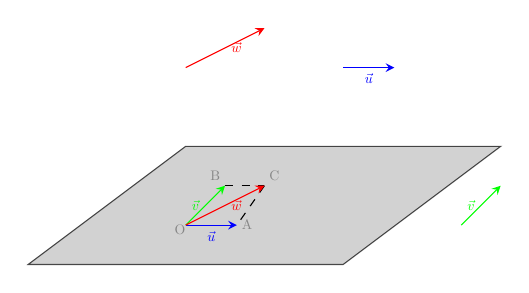
\begin{tikzpicture}
                    \coordinate (O) at (-1,0) {}; \draw (O) node[anchor=north east, scale=0.5, inner sep=0pt] {O};
                    \coordinate (A) at (-0.35,0) {}; \draw (A) node[anchor=west, scale=0.5] {A};
                    \coordinate (B) at (-0.5,0.5) {}; \draw (B) node[anchor=south east, scale=0.5] {B};
                    \coordinate (C) at (0,0.5) {}; \draw (C) node[anchor=south west, scale=0.5] {C};
                    \draw[fill=lightgray, opacity=0.7] (-3,-0.5) -- (1,-0.5) -- (3,1) -- (-1,1) -- cycle;
                    \draw[dashed] (B) -- (C);
                    \draw[dashed] (C) -- (A);
                    \draw[-stealth, blue] (O) -- (A) node [midway, label={[scale=0.5, label distance=-6pt]below:$\vec{u}$}] {};
                    \draw[-stealth, green] (O) -- (B) node [midway, label={[scale=0.5, label distance=-6pt]left:$\vec{v}$}] {};
                    \draw[-stealth, red] (O) -- (C) node [midway, label={[scale=0.5, label distance=-6pt]right:$\vec{w}$}] {};

                    \draw[-stealth, blue] (1,2) -- (1.65,2) node [midway, label={[scale=0.5, label distance=-6pt]below:$\vec{u}$}] {};
                    \draw[-stealth, green] (2.5,0) -- (3,0.5) node [midway, label={[scale=0.5, label distance=-6pt]left:$\vec{v}$}] {};
                    \draw[-stealth, red] (-1,2) -- (0,2.5) node [midway, label={[scale=0.5, label distance=-6pt]right:$\vec{w}$}] {};
                \end{tikzpicture}
                \parbox{\linewidth}{\captionof{figure}{Illustration de la Définition}}
            \end{center}
            Si $O$ est un point quelconque et $A$, $B$ et $C$ sont tels que $\overrightarrow{OA}=\vec{u},\ \overrightarrow{OB}=\vec{v},\ \text{et}\ \overrightarrow{OC}=\vec{w}$

            $\vec{u}$, $\vec{v}$, et $\vec{s}$ coplanaires $\iff$ $O$, $A$, $B$, et $C$ coplanaires
        \end{Spartie}
        \begin{Spartie}{Théorème} 
            $\vec{u}$, $\vec{v}$ et $\vec{w}$ étant trois vecteurs de l'espace avec $\vec{u}$ et $\vec{v}$ non colinéaires.

            $\vec{u}$, $\vec{v}$ et $\vec{w}$ sont coplanaires si et seulement si il existe deux réels $\alpha$ et $\beta$ tels que $\vec{w}=\alpha\vec{u}+\beta\vec{v}$. \quad\big($\vec{w}$ est une \emph{combinaison linéaire} de $\vec{u}$ et $\vec{v}$\big)
            \begin{SSpartie}{Démonstration} 
                Soient $O$, $A$, $B$, et $C$ quatre points tels que $\overrightarrow{OA}=\vec{u},~\overrightarrow{OB}=\vec{v}$ et $\overrightarrow{OC}=\vec{w}$

                $\vec{u}$ et $\vec{v}$ sont non-colinéaires donc, $O$, $A$ et $B$ sont non alignés, et $\big(OAB\big)$ est un plan de base $\left(O\,,\overrightarrow{OA}\,,\overrightarrow{OB}\right)$
                \begin{itemize}[leftmargin=7ex]
                    \item[``$\implies$''] On suppose que $\vec{u}$, $\vec{v}$, et $\vec{w}$ sont coplanaires. Alors, $C\in\big(OAB\big)$. \\ $C$ admet donc des coordonnées $\big(\alpha\,;\beta\big)$ dans la base $\left(O\,,\overrightarrow{OA}\,,\overrightarrow{OB}\right)$. C'est-à-dire $\overrightarrow{OC}=\alpha\overrightarrow{OA}+\beta\overrightarrow{OB}$ ou encore $\vec{w}=\alpha\vec{u}+\beta\vec{v}$.$\quad\square$
                    \item[``$\impliedby$''] On suppose que $\vec{w}=\alpha\vec{u}+\beta\vec{v}$ \\ Soit $D$ le point de $\big(OAB\big)$ de coordonnées $\big(\alpha\,;\beta\big)$ \\ Alors, 
                     
                    $\begin{aligned}[t]
                        \overrightarrow{OD}&=\alpha\overrightarrow{OA}+\beta\overrightarrow{OB} \\
                        &=\alpha\vec{u}+\beta\vec{v}=\vec{w}=\overrightarrow{OC}
                    \end{aligned}$

                    Donc, $D=C$, les points sont confondus, et comme $C\in\big(OAB\big)$, $\vec{u}$,~$\vec{v}$,~et~$\vec{w}$ sont coplanaires.$\quad\square$
                \end{itemize}
            \end{SSpartie}
            \begin{SSpartie}{Théorème : Caracterisation Vectorielle d'un Espace} 
                Si $A$, $B$, et $C$ sont trois points non-alignés de l'espace, le plan $\big(ABC\big)$ est l'ensemble des M tels que : \[\overrightarrow{AM}=t\overrightarrow{AB}+t'\overrightarrow{AC}\quad\big(~t,~t'\in\mathbb{R}~\big)\]
            \end{SSpartie}
        \end{Spartie}
    \end{Gpartie}
    \begin{Gpartie}{Repèrage dans l'Espace} 
        \begin{Spartie}{Définition} 
            Un repère de l'espace est constitué d'un point appelé origine du repère (en général $O$) et d'un triplet de vecteurs non-coplanaires (en général $\vec{\imath}$, $\vec{\jmath}$ et $\vec{k}$)

            On le note $\left(O\,;\vec{\imath}\,,\vec{\jmath}\,,\vec{k}\right)$
        \end{Spartie}
        \begin{Spartie}{Vocabulaire} 
            La droite $\big(O\,;\vec{\imath}\big)$ est appelée axe des \emph{abscisses}.

            La droite $\big(O\,;\vec{\jmath}\big)$ est appelée axe des \emph{ordonnées}.

            La droite $\big(O\,;\vec{k}\big)$ est appelée axe des \emph{cotes}.

            Lorsque ces trois axes sont perpendiculaires deux à deux, le repère est \emph{orthogonal}. \\ Si de plus $\lvert\lvert\vec{\imath}\rvert\rvert=\lvert\lvert\vec{\jmath}\rvert\rvert=\lvert\lvert\vec{k}\rvert\rvert=1$, le repère est \emph{orthonormé}.
        \end{Spartie}
        \begin{Spartie}{Coordonnées dans l'Espace} 
            \begin{SSpartie}{Théorème} 
                Si $\left(O\,;\vec{\imath}\,,\vec{\jmath}\,,\vec{k}\right)$ est un repère, pour tout point $M$, il existe un unique triplet $\big(x\,; y\,; z\big)$ de réels tels que $\overrightarrow{OM}=x\vec{\imath}+y\vec{\jmath}+z\vec{k}$, appelés coordonnées de $M$.

                On note $M~\big(x\,;y\,;z\big)$
                \begin{SSSpartie}{Démonstration} 
                    % \begin{center}
                        % \begin{tikzpicture}
                            % \includegraphics[width=10cm]{example-image}
                            % \parbox{\linewidth}{\captionof{figure}{Démonstration du Théorème}}        
                        % \end{tikzpicture}
                    % \end{center}
                    $\overrightarrow{OM}=\overrightarrow{OM'}+\overrightarrow{M'M}$ \\
                    Or $M\in\left(O\,;\vec{\imath}\,;\vec{\jmath}\right)$ donc il a des coordonnées $\big(x\,; y\big)$ dans le~repère~$\left(O\,;\vec{\imath}\,;\vec{\jmath}\right)$.

                    $\overrightarrow{OM'}=x\vec{\imath}+y\vec{\jmath}$

                    $\overrightarrow{M'M}$ est colinéaire à $\vec{k}$ (on a projeté dans sa direction). Il existe un réel $z$ tek que $\overrightarrow{M'M}=z\vec{k}$

                    Donc, $\overrightarrow{OM}=x\vec{\imath}+y\vec{\jmath}+z\vec{k}\quad\square$ \\
                    (On admet l'unicité)
                \end{SSSpartie}
                \begin{SSSpartie}{Remarque} 
                    On définit de même les coordonnées d'un vecteur de l'espace. Tout vecteur de l'espace est une combinaison linéaire des vecteurs $\vec{\imath}$, $\vec{\jmath}$ et $\vec{k}$.
                \end{SSSpartie}
            \end{SSpartie}
            \begin{SSpartie}{Théorème} 
                Si dans un repère $A~\big(x_A\,; y_A\,; z_A\big)$ et $B~\big(x_B\,; y_B\,; z_B\big)$ sont deux points, le vecteur $\overrightarrow{AB}$ a pour coordonnées : 
                \[\overrightarrow{AB}~\begin{psmallmatrix} x_B-x_A \\ y_B-y_A \\ z_B-z_A \end{psmallmatrix}\]
                Et $I$, le point du milieu de $\big[AB\big]$ :
                \[I~\Bigg(~\frac{x_A+x_B}{2}~;~\frac{y_A+y_B}{2}~;~\frac{z_A+z_B}{2}~\Bigg)\]
                Dans un repère orthonormé, un vecteur $\vec{u}~\begin{psmallmatrix}x \\ y \\ z\end{psmallmatrix}$ a pour norme :
                \[\lvert\lvert\vec{u}\rvert\rvert=\sqrt{x^2+y^2+z^2}\]
                \begin{SSSpartie}{Démonstration} 
                    Passer par $M'$, le projeté orthogonal de $M$ sur $\left(O\,;\vec{\imath}\,,\vec{\jmath}\right)$, puis appliquer le théorème de \textsc{Pythagore} deux fois.
                \end{SSSpartie}
            \end{SSpartie}
            \begin{SSpartie}{Théorème} 
                Si $I$ est le milieu de $\big[AB\big]$, pour tout $M$ :
                \[\overrightarrow{MI}=\tfrac{1}{2}\overrightarrow{MA}+\tfrac{1}{2}\overrightarrow{MB}\]
                \begin{SSSpartie}{Démonstration} 
                    $\begin{aligned}[t]
                        \overrightarrow{MI}&=\overrightarrow{MA}+\overrightarrow{AI} \\
                        &=\tfrac{1}{2}\overrightarrow{MA}+\tfrac{1}{2}\overrightarrow{MA}+\tfrac{1}{2}\overrightarrow{AB} \\
                        &=\tfrac{1}{2}\overrightarrow{MA}+\tfrac{1}{2}\overrightarrow{MB}\quad\text{(Chasles)}
                    \end{aligned}$
                \end{SSSpartie}
            \end{SSpartie}
        \end{Spartie}
    \end{Gpartie}








    \chapter{Succession d'Épreuves Indépendantes Loi Binomiale}

    \begin{Gpartie}{Succession d'Épreuves Indépendantes} 
        \begin{Spartie}{Rappel} 
            Deux épreuves successives sont indépendantes lorsque le résultat de la première n'influe pas sur le résultat de la deuxième.

            \begin{center} % source https://texample.net/tikz/examples/probability-tree/
                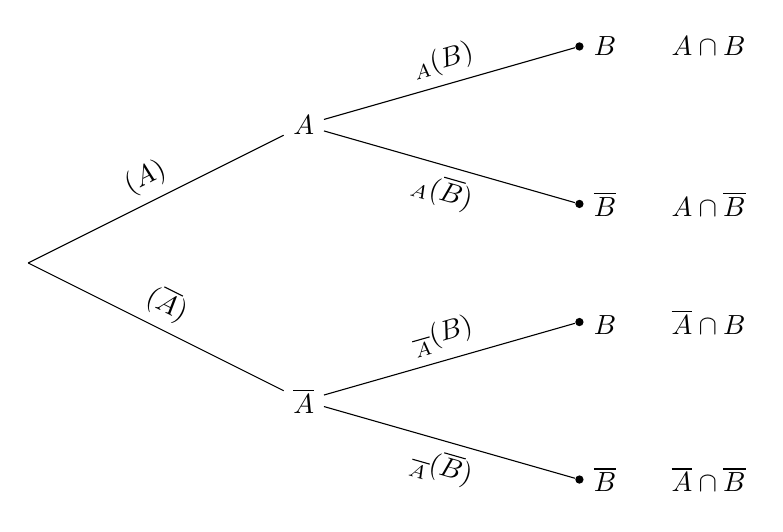
\begin{tikzpicture}[grow=right, sloped, scale=1]
                    \tikzstyle{level 1}=[level distance=3.5cm, sibling distance=3.5cm]
                    \tikzstyle{level 2}=[level distance=3.5cm, sibling distance=2cm]
                    \tikzstyle{end} = [circle, minimum width=3pt,fill, inner sep=0pt]
                    \coordinate
                        child {
                            node {$\overline{A}$}       
                                child {
                                    node[end, label=right:
                                        {$\overline{B}\qquad\overline{A}\cap\overline{B}$}] {}
                                    edge from parent
                                    node[below]  {$\Pde_{\overline{A}}(\overline{B})$}
                                }
                                child {
                                    node[end, label=right:
                                        {$B\qquad\overline{A}\cap B$}] {}
                                    edge from parent
                                    node[above] {$\Pde_{\overline{A}}({B})$}
                                }
                                edge from parent 
                                node[above] {$\Pde(\overline{A})$}
                        }
                        child {
                            node {$A$}        
                            child {
                                    node[end, label=right:
                                        {$\overline{B}\qquad A\cap\overline{B}$}] {}
                                    edge from parent
                                    node[below] {$\Pde_{A}(\overline{B})$}
                                }
                                child {
                                    node[end, label=right:
                                        {$B\qquad A\cap B$}] {}
                                    edge from parent
                                    node[above]  {$\Pde_{A}({B})$}
                                }
                            edge from parent         
                                node[above] {$\Pde(A)$}
                        };
                \end{tikzpicture}
                \parbox{\linewidth}{\captionof{figure}{Arbre de Probabilité qui Présente l'Indépendance des Épreuves}} \\[2ex]
            \end{center}
            Ainsi, $A$ et $B$ sont deux événements indépendants si et seulement si :
            \begin{itemize}
                \item $P_A(B)=P_{\overline{A}}(B)=P(B)$
                \item $P(A\cap B)=P(A)\times P(B)$
            \end{itemize}
        \end{Spartie}
        \begin{Spartie}{Modélisations} 
            On peut représenter une succession de $n$ épreuves indépendantes par un arbre pondéré (une issue de cette succession d'épreuves est alors un chemin sur l'arbre).

            Si les $n$ épreuves indépendantes ont pour univers respectifs $\Omega_1\,,\Omega_2\,,\dotsb\,,\Omega_n$, les issues de ces $n$ épreuves sont les éléments du produit cartésien $\Omega_1\times\Omega_2\times\dotsb\times\Omega_n$.
        \end{Spartie}
        \pagebreak
        \begin{Spartie}{Exemple} 
            Un restaurant propose deux entrées $e_1$ et $e_2$, trois plats $p_1$, $p_2$, et $p_3$ et un dessert $d$.

            Un client prend au hasard une entrée, un plat, et un dessert.

            L'ensemble des issues de cette expérience est $\Omega=\Omega_1\times\Omega_2\times\Omega_3$ où \\ $\Omega_1=\big\{e_1\,; e_2\big\},\ \Omega_2=\big\{p_1\,; p_2\,; p_3\big\},\text{ et }\Omega_3=\big\{d\big\}$.

            Ainsi, $\Omega=\bigg\{\big(e_1\,, p_1\,, d\big)\,;\big(e_1\,, p_2\,, d\big)\,;\dotsc\bigg\}$.

            On peut aussi représenter la situation par un arbre :
            \begin{center}
                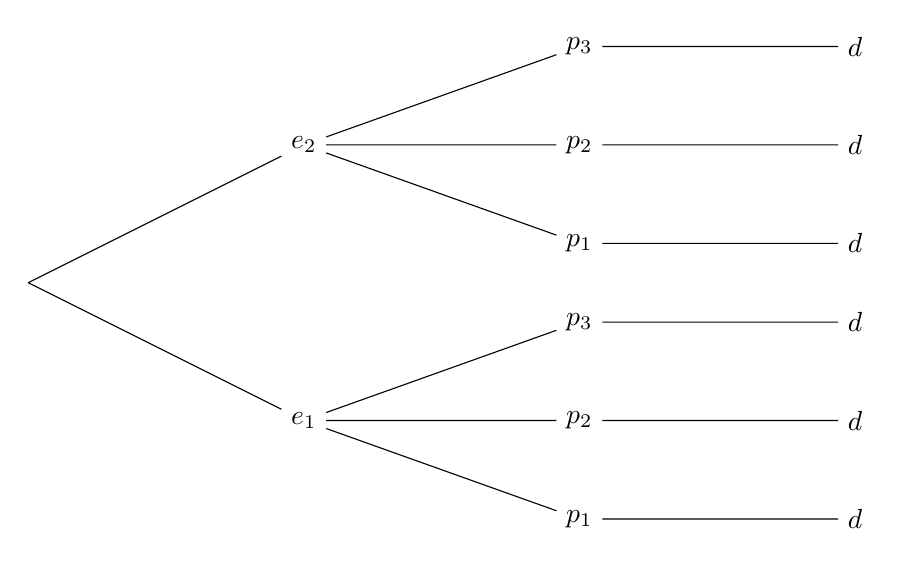
\begin{tikzpicture}[grow=right, sloped, scale=1]
                    \tikzstyle{level 1}=[level distance=3.5cm, sibling distance=3.5cm]
                    \tikzstyle{level 2}=[level distance=3.5cm, sibling distance=1.25cm]
                    \tikzstyle{level 3}=[level distance=3.5cm]
                    \tikzstyle{end} = [circle, minimum width=3pt,fill, inner sep=0pt]
                    \coordinate
                        child {
                            node {$e_1$}       
                                child {
                                    node {$p_1$} child { node {$d$} }
                                }
                                child {
                                    node {$p_2$} child { node {$d$} }
                                }
                                child {
                                    node {$p_3$} child { node {$d$} }
                                }
                        }
                        child {
                            node {$e_2$}        
                                child {
                                    node {$p_1$} child { node {$d$} }
                                }
                                child {
                                    node {$p_2$} child { node {$d$} }
                                }
                                child {
                                    node {$p_3$} child { node {$d$} }
                                }
                        };
                \end{tikzpicture}
                \parbox{\linewidth}{\captionof{figure}{Arbre Pondéré Représentant la Situation}}
            \end{center}
        \end{Spartie}
    \end{Gpartie}
    \vfill\pagebreak
    \begin{Gpartie}{Loi Binomiale} 
        \begin{Spartie}{Épreuve de Bernoulli} 
            \begin{SSpartie}{Définition} 
                Une \emph{épreuve de} \textsc{Bernoulli} est un expérience aléatoire possédant deux issues qu'on appelle généralement \og succès \fg{} et \og échec \fg{}. La probabilité du succès $p$ est appelée paramètre de la loi de \textsc{Bernoulli}.
                \begin{center}
                    \begin{tabular}{  | p{0.1\textwidth} || *{2}{w{c}{0.1\textwidth} | }  } \hline
                        $k_i$           & $0$ & $1$ \\ \hline
                        $P(X=k_i)$      &$1-p$& $p$ \\ \hline
                    \end{tabular}
                    \parbox{\linewidth}{\captionof{figure}{Loi de la Variable Aléatoire X}}
                \end{center}
                $X$ est une variable aléatoire donnant le nombre de succès (il n'y a que deux possibilités : 0 ou 1). On dit que $X$ suit la loi de \textsc{Bernoulli}. \\ Penser à un jeu de pile ou face.
            \end{SSpartie}
            \begin{SSpartie}{Propriété} 
                Si $X$ est une variable aléatoire suivant la loi de \textsc{Bernoulli} de paramètre $p$, alors, l'espérance de $X$ est $E(X)=p$ et sa variance est $V(X)=p(1-p)$.
            \end{SSpartie}
        \end{Spartie}
        \begin{Spartie}{Schéma de Bernoulli} 
            \begin{SSpartie}{Définition} 
                Un \emph{schéma de} \textsc{Bernoulli} est une répétition de $n$ épreuves \emph{identiques} et \emph{indépendantes} à deux issues ($n$ épreuves de \textsc{Bernoulli}).

                Une issue de cette expérience aléatoire est un élément ($n$-uplet) de $\Omega=\big\{S\,;\overline{S}\big\}^n$.
            \end{SSpartie}
            \begin{SSpartie}{Exemple} 
                On tire successivement $4$ fois à pile ou face avec une pièce (truquée peut-être) dont la probabilité de tomber sur \og pile \fg{} est $p$. 
                
                Les tirages obtenus sont des 4-uplets composés de $P$ et de $F$ (si l'on note $P$ l'événement \og tomber sur pile \fg{} et $F$ \og tomber sur face \fg{}).
                
                Un exemple de tirage est $\big(P\,, F\,, F\,, F\big)$. On peut aussi noter $S$ et $\overline{S}$ au lieu de $P$ et $F$.
            \end{SSpartie}
        \end{Spartie}
        \begin{Spartie}{Loi Binomiale} 
            \begin{SSpartie}{Définition} 
                On considère une expérience aléatoire qui suit un schéma de \textsc{Bernoulli}, autrement dit, une répétition de $n$ épreuves \emph{identiques} et \emph{indépendantes} à deux issues (succès et échec) dont la probabilité de succès est $p$.

                La variable aléatoire donnant le nombre de succès suit la \emph{loi binomiale} de paramètres $n$ et $p$, notée $\mathcal{B}(n\,, p)$. Cette loi est aussi parfois appelée loi du nombre de succès.
            \end{SSpartie}
            \begin{SSpartie}{Propriété} 
                Soit $X$ une variable aléatoire suivant la loi binomiale de paramètres $n$ et $p$, on peut aussi noter $X\sim\mathcal{B}(n\,, p)$.

                Pour tout entier $k$ compris entre $0$ et $n$ :
                \[\boxed{P(X=k)=\binom{n}{k}p^k(1-p)^{n-k}}\]

                \begin{center}
                    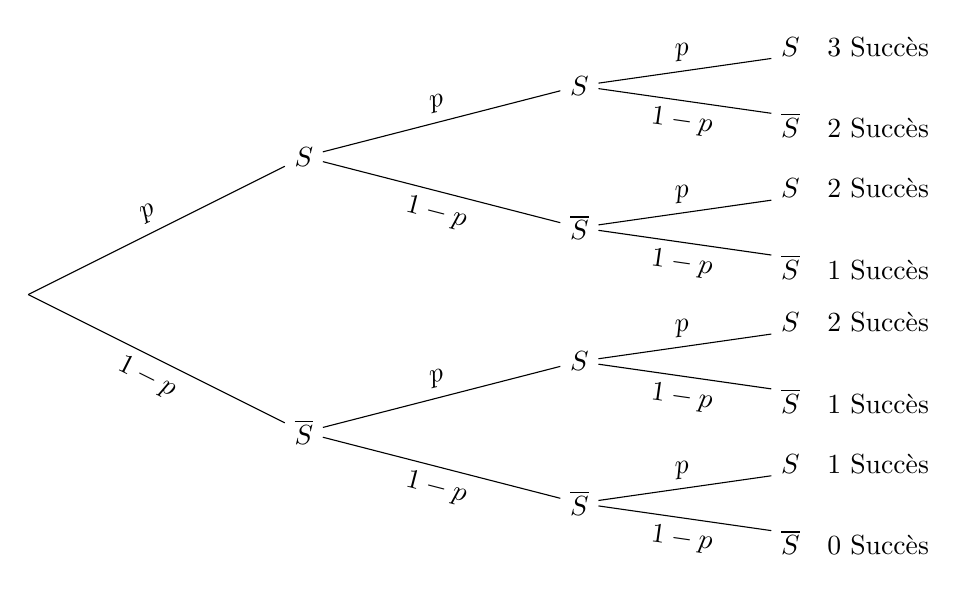
\begin{tikzpicture}[grow=right, sloped, scale=1]
                        \tikzstyle{level 1}=[level distance=3.5cm, sibling distance=3.5cm]
                        \tikzstyle{level 2}=[level distance=3.5cm, sibling distance=1.8cm]
                        \tikzstyle{level 3}=[level distance=3.5cm, sibling distance=1cm]
                        \tikzstyle{end} = [circle, minimum width=3pt,fill, inner sep=0pt]
                        \coordinate
                            child {
                                node {$\overline{S}$}        
                                    child {
                                        node {$\overline{S}$} 
                                            child {
                                                node {$\overline{S}$\quad 0 Succès}
                                                edge from parent node[below] {$1-p$}
                                            }
                                            child {
                                                node {$S$\quad 1 Succès}
                                                edge from parent node[above] {$p$}
                                            } 
                                        edge from parent node[below] {$1-p$}
                                    }
                                    child {
                                        node {$S$} 
                                            child {
                                                node {$\overline{S}$\quad 1 Succès}
                                                edge from parent node[below] {$1-p$}
                                            }
                                            child {
                                                node {$S$\quad 2 Succès}
                                                edge from parent node[above] {$p$}
                                            }
                                        edge from parent node[above] {$p$}
                                    }
                                edge from parent node[below] {$1-p$}
                            }
                            child {
                                node {$S$}        
                                    child {
                                        node {$\overline{S}$} 
                                            child {
                                                node {$\overline{S}$\quad 1 Succès}
                                                edge from parent node[below] {$1-p$}
                                            }
                                            child {
                                                node {$S$\quad 2 Succès}
                                                edge from parent node[above] {$p$}
                                            } 
                                        edge from parent node[below] {$1-p$}
                                    }
                                    child {
                                        node {$S$} 
                                            child {
                                                node {$\overline{S}$\quad 2 Succès}
                                                edge from parent node[below] {$1-p$}
                                            }
                                            child {
                                                node {$S$\quad 3 Succès}
                                                edge from parent node[above] {$p$}
                                            } 
                                        edge from parent node[above] {$p$}
                                    }
                                edge from parent node[above] {$p$}
                            };
                    \end{tikzpicture}
                        \parbox{\linewidth}{\captionof{figure}{Illustration de la Loi Binomiale}}
                \end{center}
                \begin{SSSpartie}{Démonstration} 
                    Dans l'arbre, chaque chemin contenant exactement $k$ succès passe par $k$ branches de probabilité $p$ et $n-k$ branches de probabilité $1-p$. Ainsi la probabilité d'un tel chemin est $p^k(1-p)^{n-k}$.

                    On compte ensuite le nombre de chemins contenant $k$ succès : il~y~en~a~$\binom{n}{k}$.

                    On peut aussi considérer qu'un tirage est un $n$-uplet contenant des $S$ et des $\overline{S}$.

                    Ainsi, un tirage contenant $k$ succès comporte $k$ fois la lettre $S$ et $n-k$ fois la lettre $\overline{S}$. Le nombre de façons de disposer les $k$ \og $S$ \fg{} parmi les $n$ éléments est $\binom{n}{k}$.
                \end{SSSpartie}
                \begin{SSSpartie}{Exemple} 
                    Avec nos $4$ tirages de pièce truquée, si on a $p=\frac{2}{3}$ (la probabilité de tirer \og pile \fg{} est $\frac{2}{3}$) et si on note $X$ la variable aléatoire donnant le nombre de \og pile \fg{}, on a :
                    \[P\big(X=1\big)=\binom{4}{1}\Bigg(\frac{2}{3}\Bigg)^1\Bigg(1-\frac{2}{3}\Bigg)^{4-1}=4\times\Bigg(\frac{2}{3}\Bigg)\times\Bigg(\frac{1}{3}\Bigg)^3\approx 0{,}099\]
                \end{SSSpartie}
            \end{SSpartie}
            \begin{SSpartie}{Propriété} 
                Soit $X$ une variable aléatoire suivant la loi binomiale $\mathcal{B}(n\,, p)$.

                L'Espérance de $X$ est $\boxed{E(X)=np}$ \\ La variance de $X$ est $\boxed{V(X)=np(1-p)}$ \\ L'Écart-type de $X$ est $\boxed{\sigma(X)=\sqrt{np(1-p)}}$

                Démonstration dans chapitre sur les opérations sur les Variables Aléatoires.
                \begin{SSSpartie}{Exemple} 
                    On reprend la pièce truquée précédente, qu'on lance quatre fois. $X$ est toujours la variable aléatoire donnant le nombre de \og pile \fg.

                    $E(X)=4\times\frac{2}{3}\approx 2{,}67$\quad (On peut espérer d'obtenir 2{,}67 piles sur 4 tirages).

                    $\sigma(X)=\sqrt{4\times\frac{2}{3}\times\frac{1}{3}}\approx 0{,}94$\quad (Dont l'interprétation est moins intéressante).
                \end{SSSpartie}
            \end{SSpartie}
        \end{Spartie}
    \end{Gpartie}






    \chapter{Limites de Fonctions}

    \begin{Gpartie}{Limites d'une Fonction en l'Infini} 
        \begin{Spartie}{Limite en $+\infty$} 
            \begin{SSpartie}{Définitions} 
                Soit une fonction $f$ définie au moins sur $\big[a~;+\infty\big[$, où $a$ est un réel.

                \begin{itemize}
                    \item   On dit que $f$ a pour limite $+\infty$ en $+\infty$ si pour tout réel $M$ positif, il existe un réel $A$, tel que $x>A$ implique $f(x)\geq M$. \\ Autrement dit, lorsque $x$ prend des valeurs de plus en plus grandes, $f(x)$ peut être aussi grand que l'on veut.
                    
                    On note : \[\boxed{\lim\limits_{x\to +\infty}f(x)=+\infty}\] 
                    \begin{center}
                        \begin{tikzpicture}[scale=0.8]
                            \begin{axis}[
                                xmin=-2, xmax=4,
                                ymin=-1, ymax=6,
                                xtick=\empty,
                                ytick=\empty
                            ]
                                \addplot[black]{5};
                                \draw (0,5) node[anchor=north east] {M};
                                \draw[thin, dashed] (3.1,0) node[dot,label={[label distance=-2pt]below:$A$}] {} -- (3.1,5);
                                \addplot[blue, very thick, samples=50]{e^(x-1.5)};
                            \end{axis}
                        \end{tikzpicture}
                        \parbox{\linewidth}{\captionof{figure}{\centering Représentation Graphique d'une Fonction qui Semble Tendre vers $+\infty$ en $+\infty$}}
                    \end{center}
                    \pagebreak
                    \item   On dit que $f$ a pour limite $-\infty$ en $+\infty$ si pout tout réel $m$ négatif, il existe un réel $A$, tel que $x>A$, $f(x)\leq m$. \\ Autrement dit, lorsque $x$ prend des valeurs de plus en plus grandes, $f(x)$ est négatif et peut être aussi grand que l'on veut en valeur absolue.
                    
                    On note : \[\boxed{\lim\limits_{x\to +\infty}f(x)=-\infty}\]
                    \begin{center}
                        \begin{tikzpicture}[scale=0.8]
                            \begin{axis}[
                                xmin=-2, xmax=4,
                                ymin=-6, ymax=1,
                                xtick=\empty,
                                ytick=\empty
                            ]
                                \draw (0,-5) node[anchor=north east] {m};
                                \draw[thin, dashed] (3.1,0) node[dot,label={[label distance=-2pt]above:$A$}] {} -- (3.1,-5);
                                \addplot[black]{-5};
                                \addplot[blue, very thick, samples=50]{-e^(x-1.5)};
                            \end{axis}
                        \end{tikzpicture}
                        \parbox{\linewidth}{\captionof{figure}{\centering Représentation Graphique d'une Fonction qui Semble Tendre vers $-\infty$ en $+\infty$}}
                    \end{center}
                    \item   On dit que $f$ a pour limite $\ell$ en $+\infty$ où $\ell$ est un réel si pour tout intervalle ouvert $I$ contenant $\ell$, il existe un réel $A$ tel que $x>A$ implique $f(x)\in I$ \\ Autrement dit, lorsque $x$ prend des valeurs de plus en plus grandes, $f(x)$ peut être aussi près de $\ell$ que l'on veut.
                    
                    On note : \[\boxed{\lim\limits_{x\to +\infty}f(x)=\ell}\]
                    \begin{center}
                        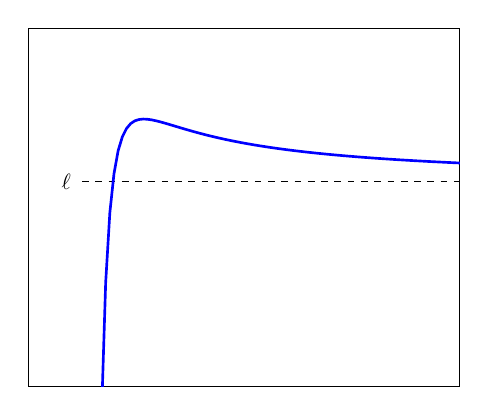
\begin{tikzpicture}[scale=0.8]
                            \begin{axis}[
                                xmin=-0.5, xmax=3.5,
                                ymin=-1, ymax=2.5,
                                xtick=\empty,
                                ytick=\empty,
                                domain=0.18:4
                            ]
                            \draw[thin, dashed] (0,1) node[label={[label distance=-2pt]left:$\ell$}] {} -- (3.5,1);
                                \addplot[blue, very thick, samples=100]{0.7*\x^(-1)-1/5*\x^(-2)+1};
                            \end{axis}
                        \end{tikzpicture}
                        \parbox{\linewidth}{\captionof{figure}{\centering Représentation Graphique d'une Fonction qui Semble Tendre vers $\ell$ en $+\infty$}}
                    \end{center}
                    H.P.: $\forall\epsilon >0,~\exists A\in\mathbb{R},~\forall x\in\mathcal{D}_f$ \\ \phantom{H.P.: }$\bigg(x>A\implies\left\lvert f(x)-l\right\rvert <\epsilon\bigg)$ ou $\bigg(x>A\implies f(x)\in\big]l-\epsilon~;l+\epsilon\big[\bigg)$
                \end{itemize}
            \end{SSpartie}
            \pagebreak
            \begin{SSpartie}{Définition} 
                Soit $f$ une fonction définie au moins sur $\big[A~;+\infty\big[$, où $A$ est un réel, et $\mathcal{C}$ sa courbe représentative dans un repère. \\ Si $\lim\limits_{x\to+\infty}f(x)=\ell$ alors $\mathcal{C}$ admet une \emph{asymptote horizontale} en $+\infty$ \\ d'équation $y=\ell$.
            \end{SSpartie}
            \begin{SSpartie}{Remarque} 
                Une fonction n'admet pas forcément de limite en $+\infty$, par exemple, les fonctions sinus et cosinus sont bornées et n'admettent pas de limites en l'infini.
            \end{SSpartie}
        \end{Spartie}
        \begin{Spartie}{Limite en $-\infty$} 
            \begin{SSpartie}{Définitions}
                Soit $f$ une fonction définie au moins sur $\big]-\infty~;a\big[$, où $a$ est un réel.
                \begin{itemize}
                    \item   On dit que $f$ a pour limite $+\infty$ en $-\infty$ si pour tout réel $M$, positif, il existe un réel $A$ tel que $x<A$ implique $f(x)\geq M$ \\ Autrement dit, lorsque $x$ prend des valeurs négatives de plus en plus grandes en valeur absolue, $f(x)$ peut être aussi grand que l'on veut.
                    
                    On note : \[\boxed{\lim\limits_{x\to-\infty}f(x)=+\infty}\]
                    \begin{center}
                        \begin{tikzpicture}[scale=0.8]
                            \begin{axis}[
                                xmin=-4, xmax=2,
                                ymin=-1, ymax=6,
                                xtick=\empty,
                                ytick=\empty,
                                domain=-4:1.75
                            ]
                                \addplot[black]{5};
                                \draw (0,5) node[anchor=north west] {M};
                                \draw[thin, dashed] (-3.1,0) node[dot,label={[label distance=-2pt]below:$A$}] {} -- (-3.1,5);
                                \addplot[blue, very thick, samples=50]{e^(-x-1.5)};
                            \end{axis}
                        \end{tikzpicture}
                        \parbox{\linewidth}{\captionof{figure}{\centering Représentation Graphique d'une Fonction qui Semble Tendre vers $+\infty$ en $-\infty$}}
                    \end{center}
                    \pagebreak
                    \item   On dit que $f$ a pour limite $-\infty$ en $-\infty$ si pour tout réel $m$ négatif, il existe un réel $A$ tel que $x<A$ implique $f(x)\leq m$ \\ On note : \[\boxed{\lim\limits_{x\to-\infty}f(x)=-\infty}\]
                    \begin{center}
                        \begin{tikzpicture}[scale=0.7]
                            \begin{axis}[
                                xmin=-4, xmax=2,
                                ymin=-6, ymax=1,
                                xtick=\empty,
                                ytick=\empty
                            ]
                                \draw (0,-5) node[anchor=north east] {m};
                                \draw[thin, dashed] (-3.1,0) node[dot,label={[label distance=-2pt]above:$A$}] {} -- (-3.1,-5);
                                \addplot[black]{-5};
                                \addplot[blue, very thick, samples=50]{-e^(-x-1.5)};
                            \end{axis}
                        \end{tikzpicture}
                        \parbox{\linewidth}{\captionof{figure}{\centering Représentation Graphique d'une Fonction qui Semble Tendre vers $-\infty$ en $-\infty$}}
                    \end{center}
                    \item   On dit que $f$ a pour limite $\ell$ en $-\infty$ où $\ell$ est un réel, si pour tout intervalle ouvert $I$ contenant $\ell$, on peut trouver un réel $A$ tel que si $x\leq A$, $f(x)$ appartient à $I$. \\ Autrement dit, lorsque $x$ prend des valeurs négatives, de plus en plus grandes en valeur absolue, $f(x)$ peut être aussi près de $\ell$ que l'on veut.
                    
                    On note : \[\boxed{\lim\limits_{x\to-\infty}f(x)=\ell}\]
                    \begin{center}
                        \begin{tikzpicture}[scale=0.7]
                            \begin{axis}[
                                xmin=-3.5, xmax=0.5,
                                ymin=-0.5, ymax=3,
                                xtick=\empty,
                                ytick=\empty,
                                domain=-3.5:-0.1
                            ]
                                \draw[thin, dashed] (0,1) node[label={[label distance=-2pt]right:$\ell$}] {} -- (-3.5,1);
                                \addplot[blue, very thick, samples=100]{-1/\x+1};
                            \end{axis}
                        \end{tikzpicture}

                        \parbox{\linewidth}{\captionof{figure}{\centering Représentation Graphique d'une Fonction qui Semble Tendre vers $2$ en $-\infty$}}
                    \end{center}
                    H.P.: $\forall\epsilon >0,~\exists A\in\mathbb{R},~\forall x\in\mathcal{D}_f$ \\ \phantom{H.P.: }$\bigg(x<A\implies\left\lvert f(x)-\ell\right\rvert <\epsilon\bigg)$ ou $\bigg(x<A\implies f(x)\in\big]\ell-\epsilon~;\ell+\epsilon\big[\bigg)$
                \end{itemize}
            \end{SSpartie}
            \begin{SSpartie}{Définition} 
                Si $\mathcal{C}$ est la courbe représentative de $f$ dans un repère. $\lim\limits_{x\to-\infty}f(x)=\ell$ alors $\mathcal{C}$ admet une \emph{asymptote horizontale} en $-\infty$ d'équation $y=\ell$.
            \end{SSpartie}
        \end{Spartie}
    \end{Gpartie}
    \pagebreak
    \begin{Gpartie}{Limite d'une Fonction en un Réel} 
        \begin{Spartie}{Définitions} 
            Soit $a$ un réel et $f$ une fonction définie sur un intervalle $I$ contenant $a$ ou tel que $a$ est une borne de $I$.

            Si, lorsque $x$ prend des valeurs de plus en plus proches de $a$ :
            \begin{itemize}
                \item $f(x)$ est aussi grand que l'on veut, on dit que $f$ a pour limite $+\infty$ en $a$.

                On note : \[\boxed{\lim\limits_{x\to a}f(x)=+\infty}\]
                \begin{center}
                    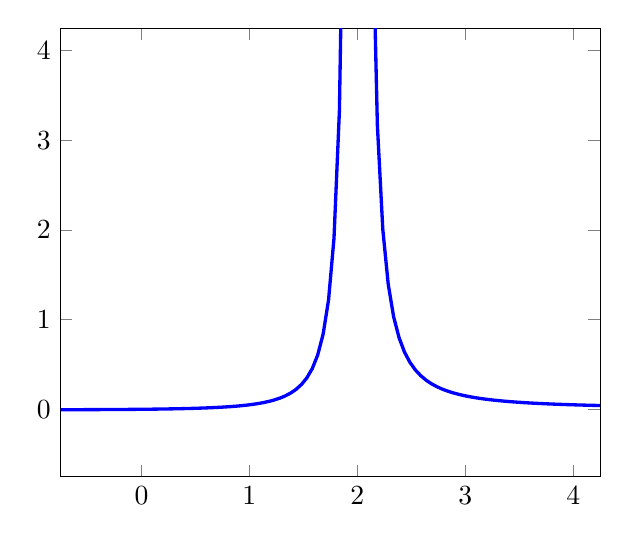
\begin{tikzpicture}
                        \begin{axis}[
                            xmin=-0.75, xmax=4.25,
                            ymin=-0.75, ymax=4.25,
                            restrict y to domain =-20:20
                        ]
                            \addplot[blue, very thick, samples=200]{\x*(x-2)^(-2)*1/(20)};
                        \end{axis}
                    \end{tikzpicture}
                    \parbox{\linewidth}{\captionof{figure}{\centering Représentation Graphique d'une Fonction qui Semble Tendre vers $+\infty$ en $2$}}
                \end{center}
                \item $f(x)$ est négatif et aussi grand que l'on veut en valeur absolue, on dit que $f$ a pour limite $-\infty$ en $a$.

                On note : \[\boxed{\lim\limits_{x\to a}f(x)=-\infty}\]
                \item $f(x)$ est aussi proche que l'on veut d'un réel $\ell$, on dit que $f$ a pour limite $\ell$ en $a$.
                
                On note : \[\boxed{\lim\limits_{x\to a}f(x)=\ell}\]
            \end{itemize}
            \begin{SSpartie}{Remarque} 
                Si $f$ est \emph{continue} en $a$, $\ell=f(a)$.
            \end{SSpartie}
        \end{Spartie}
        \pagebreak
        \begin{Spartie}{Limite à Droite ou à Gauche d'une Fonction en un Réel} 
            \begin{SSpartie}{Exemple} 
                La fonction $f:x\mapsto\frac{1}{x}$ n'a pas de limite en $0$ car lorsque $x$ tend vers $0$ par des valeurs positives, $\frac{1}{x}$ tend vers $+\infty$ et lorsque $x$ tend vers $0$ par valeurs négatives, $\frac{1}{x}$ tend vers $-\infty$.

                Cependant, on peut parler de limite à gauche et limite à droite.

                On note : \[\lim\limits_{\substack{x\to 0 \\ x>0}}\frac{1}{x}=+\infty\qquad\lim\limits_{\substack{x\to 0 \\ x<0}}\frac{1}{x}=-\infty\]
            \end{SSpartie}
            \begin{SSpartie}{Remarque} 
                Une fonction admet une limite en un réel $a$ si la limite à droite et à gauche de $f$ en $a$ existent et sont égales.
            \end{SSpartie}
        \end{Spartie}
        \begin{Spartie}{Asymptote Verticale} 
            \begin{SSpartie}{Définition} 
                Soit $\mathcal{C}$ la courbe représentative de la fonction $f$. Dire que $\mathcal{C}$ admet une asymptote verticale d'équation $x=a$, c'est dire que : \[\lim\limits_{x\to a}f(x)=\pm\infty\quad\text{ou}\quad\lim\limits_{\substack{x\to a \\ x>a}}f(x)=\pm\infty\quad\text{ou}\quad\lim\limits_{\substack{x\to a \\ x<a}}f(x)=\pm\infty\]
            \end{SSpartie}
        \end{Spartie}
    \end{Gpartie}
    \begin{Gpartie}{Fonctions Usuelles} 
        \begin{Spartie}{Théorème} 
            \begin{SSpartie}{Fonction Racine Carrée} 
                $\lim\limits_{x\to+\infty}\sqrt{x}=+\infty$ et $\lim\limits_{x\to0}\sqrt{x}=0$ (la fonction racine carrée est continue en $0$)
            \end{SSpartie}
            \begin{SSpartie}{Fonction Inverse} 
                $\lim\limits_{x\to+\infty}\frac{1}{x}=0,\quad\lim\limits_{\substack{x\to 0 \\ x>0}}\frac{1}{x}=+\infty,\quad\lim\limits_{\substack{x\to 0 \\ x<0}}\frac{1}{x}=-\infty,\quad\lim\limits_{x\to-\infty}\frac{1}{x}=0$
            \end{SSpartie}
            \begin{SSpartie}{Fonctions Puissances} 
                Quel que soit $p\in\mathbb{N^*},~\lim\limits_{x\to+\infty}x^p=+\infty$.

                Si $p$ est pair, $\lim\limits_{x\to-\infty}x^p=+\infty$ et si $p$ est impair, $\lim\limits_{x\to-\infty}x^p=-\infty$.
                
                Quel que soit $p\in\mathbb{N^*},~\lim\limits_{x\to+\infty}\frac{1}{x^p}=0$, et $\lim\limits_{x\to-\infty}\frac{1}{x^p}=0$.

                Si $p$ est pair, $\lim\limits_{x\to0}\frac{1}{x^p}=+\infty$ et si $p$ est impair, $\lim\limits_{\substack{x\to0 \\ x>0}}\frac{1}{x^p}=+\infty$ et $\lim\limits_{\substack{x\to0 \\ x<0}}\frac{1}{x^p}=-\infty$.
            \end{SSpartie}
            \begin{SSpartie}{Fonction Exponentielle} 
                $\lim\limits_{x\to+\infty}\me^x=+\infty,\quad\lim\limits_{x\to-\infty}\me^x=0$
            \end{SSpartie}
            \begin{SSpartie}{Fontion Logarithme Népérien} 
                $\lim\limits_{x\to+\infty}\ln\,(x)=+\infty,\quad\lim\limits_{\substack{x\to0 \\ x>0}}\ln\,(x)=-\infty$
            \end{SSpartie}
        \end{Spartie}
        \begin{Spartie}{Théorèmes de Croissance Comparée} 
            \[\lim\limits_{x\to+\infty}\frac{\me^x}{x}=+\infty\qquad\lim\limits_{x\to-\infty}x\me^x=0\]
            \begin{SSpartie}{Démonstration} 
                \begin{itemize}
                    \item On montre que $\me^x>\frac{x^2}{2}$, pour tout $x>0$ en étudiant la différence.

                    Soit $f$ définie sur $\big]0~;+\infty\big[$ par $f(x)=\me^x-\frac{x^2}{2}$. Étudions les variations de $f$.

                    $f'(x)=\me^x-x$ on ne conclut pas directement sur le signe. Dérivons encore :

                    $f''(x)=\me^x-1\quad\text{et}\quad \me^x-1>0\iff \me^x>1\iff x>0$

                    Donc, $f''(x)$ est strictement positive pour $x>0$.

                    Ainsi on a $f'(x)$ strictement croissante sur $\big]0~;+\infty\big[$ et comme $f'(0)=1>0$, $f'$ est strictement positive sur $\big]0~;+\infty\big[$ :
                    \begin{center}                        
                        \begin{tikzpicture}
                            \tkzTabInit{$x$ /1, $f''(x)$ /1, $f'(x)$ /1, $f(x)$ /1}{$0$, $+\infty$}
                            \tkzTabLine{z,+,}
                            \tkzTabVar{-/$1$,+/}
                            \tkzTabVar{-/$1$,+/}
                        \end{tikzpicture}
                        \parbox{\linewidth}{\captionof{figure}{\centering Tableau de Variation de $f$ et $f'$}}
                    \end{center}
                    Donc, pour tout $x\in\big]0~;+\infty\big[,~\me^x-\frac{x^2}{2}>0$ et donc $\me^x>\frac{x^2}{2}$ \\ Comme $x>0$ on peut diviser par $x$ : \\ Donc, $\frac{\me^x}{x}>\frac{x}{2}$ et comme $\lim\limits_{x\to+\infty}\frac{x}{2}=+\infty$, par comparaison : \[\lim\limits_{x\to+\infty}\frac{\me^x}{x}=+\infty\quad\square\]
                    \item On pose $X=-x$ et alors, $\lim\limits_{x\to-\infty}X=+\infty$ et $x\me^x=-X\me^{x}=-\frac{X}{\me^X}$
                    
                    Donc, par passage à l'inverse de la limite précédente : 
                    \[\lim\limits_{x\to-\infty}x\me^x=\lim\limits_{X\to+\infty}-\frac{X}{\me^X}=0\quad\square\]
                \end{itemize}
            \end{SSpartie}
        \end{Spartie}
        \begin{Spartie}{Théorème} 
            Quel que soit l'entier $n>0$ : \[\lim\limits_{x\to_\infty}\frac{\me^x}{x^n}=+\infty\quad\text{et}\quad\lim\limits_{x\to-\infty}x^n\me^x=0\]
        \end{Spartie}
        \begin{Spartie}{Théorèmes de Croissance Comparée (bis)} 
            \[\lim\limits_{x\to+\infty}\frac{\ln\,(x)}{x}=0\quad\text{et}\quad\lim\limits_{\substack{x\to0 \\ x>0}}x\ln\,(x)=0\]
            \begin{SSpartie}{Démonstration} 
                On pose le changement de variable $X=\ln\,(x)$ et donc $x=\me^X$. On a alors $\lim\limits_{x\to+\infty}X=+\infty$ et $\lim\limits_{\substack{x\to0 \\ x>0}}X=-\infty$.
            \end{SSpartie}
        \end{Spartie}
    \end{Gpartie}
    \begin{Gpartie}{Opérations sur les Limites} 
        \begin{Spartie}{Limites de Somme, Produit et Quotient} 
            Dans cette sous-partie, les limites des fonctions $f$ et $g$ sont prises soit en $-\infty$, soit en $+\infty$ soit en un réel $a$. $\ell$ et $\ell'$ sont des nombres réels. \\ Lorsqu'il n'y a pas de conclusion en général, on dit alors qu'il y a un cas de forme indéterminée. (F.I.) \\
            N.B.: $\pm\infty$ désigne $+\infty$ ou $-\infty$.
            \begin{SSpartie}{Limite de Somme} 
                % \begin{center}\begin{tabular}{ |m{0.15\linewidth}||*{6}{>{\centering\arraybackslash}m{0.1\linewidth}| }} \hline
                %     Si $\lim f$     & $\ell$        & $\ell$    & $\ell$    & $+\infty$ & $-\infty$ & $+\infty$ \\\hline
                %     Si $\lim g$     & $\ell'$       & $+\infty$ & $-\infty$ & $+\infty$ & $-\infty$ & $-\infty$ \\\hline
                %     $\lim (f+g)$    & $\ell+\ell'$  & $+\infty$ & $-\infty$ & $+\infty$ & $-\infty$ & F.I.      \\\hline
                % \end{tabular}\end{center}
                % \parbox{\linewidth}{\captionof{figure}{\centering Tableau des Limites de Sommes de Fonctions}}
                \begin{table}[H]
                    \centering \captionabove{Tableau des Limites de Sommes de Fonctions}
                    \resizebox{0.85\linewidth}{!}{
                        \begin{tabular}{ p{0.15\linewidth} *{3}{M{0.17\linewidth}} } \toprule
                            {} & \multicolumn{3}{c}{$\lim f$} \\ \cmidrule(l r){2-4}
                            $\lim g$    & $\ell$        & $+\infty$ & $-\infty$ \\ \midrule
                            $\ell'$     & $\ell+\ell'$  & $+\infty$ & $-\infty$ \\
                            $+\infty$   & $+\infty$     & $+\infty$ & F.I.      \\
                            $-\infty$   & $-\infty$     & F.I.      & $-\infty$ \\ \bottomrule
                        \end{tabular}
                    }
                \end{table}
            \end{SSpartie}
            \pagebreak
            \begin{SSpartie}{Limite d'un Produit} 
                % \begin{center}\begin{tabular}{ |m{0.12\linewidth}||*{9}{>{\centering\arraybackslash}m{0.061\linewidth}| }} \hline
                %     Si $\lim f$         & $\ell$            & $\ell>0$  & $\ell>0$  & $\ell<0$  & $\ell<0$  & $+\infty$ & $+\infty$ & $-\infty$ & $0$ \\\hline
                %     Si $\lim g$         & $\ell'$           & $+\infty$ & $-\infty$ & $+\infty$ & $-\infty$ & $+\infty$ & $-\infty$ & $-\infty$ & $\pm\infty$ \\\hline
                %     $\lim (fg)$  & $\ell\times\ell'$ & $+\infty$ & $-\infty$ & $-\infty$ & $+\infty$ & $+\infty$ & $-\infty$ & $-\infty$ & F.I. \\\hline
                % \end{tabular}\end{center}
                % \parbox{\linewidth}{\captionof{figure}{\centering Tableau des Limites des Produits de Fonctions}}
                \begin{table}[H]
                    \centering \captionabove{Tableau des Limites des Produits de Fonctions}
                    \resizebox{0.85\linewidth}{!}{
                        \begin{tabular}{ p{0.15\linewidth} *{6}{M{0.1\linewidth}}  } \toprule
                            {} & \multicolumn{5}{c}{$\lim f$} \\ \cmidrule(l r){2-7}
                            $\lim g$    & $\ell$        & $\ell>0$      & $\ell<0$      & $+\infty$ & $-\infty$ & $0$       \\ \midrule
                            $\ell'$     & $\ell\ell'$   & $\ell\ell'$   & $\ell\ell'$   & $+\infty$ & $-\infty$ & $0$       \\
                            $\ell'>0$   & $\ell\ell'$   & $\ell\ell'$   & $\ell\ell'$   & $+\infty$ & $-\infty$ & $0$       \\
                            $\ell'<0$   & $\ell\ell'$   & $\ell\ell'$   & $\ell\ell'$   & $-\infty$ & $+\infty$ & $0$       \\
                            $+\infty$   & $+\infty$     & $+\infty$     & $-\infty$     & $+\infty$ & $-\infty$ & F.I.      \\
                            $-\infty$   & $-\infty$     & $-\infty$     & $+\infty$     & $-\infty$ & $+\infty$ & F.I.      \\
                            $0$         & $0$           & $0$           & $0$           & F.I.          & F.I.  & $0$       \\ \bottomrule
                            
                        \end{tabular}
                    }
                \end{table}
            \end{SSpartie}
            \begin{SSpartie}{Limite d'un Quotient $f/g$} 
                % \begin{center}\begin{tabular}{ |m{0.15\linewidth}||*{7}{>{\centering\arraybackslash}m{0.082\linewidth}| }} \hline
                %     Si $\lim f$     & $\ell$                & $\ell$        & $+\infty$ & $+\infty$ & $-\infty$ & $-\infty$ & $\pm\infty$ \\\hline
                %     Si $\lim g$     & $\ell'\neq0$          & $\pm\infty$   & $\ell'>0$ & $\ell'<0$ & $\ell'>0$ & $\ell'<0$ & $\pm\infty$ \\\hline
                %     $\lim (f/g)$    & $\frac{\ell}{\ell'}$  & $0$           & $+\infty$ & $-\infty$ & $-\infty$ & $+\infty$ & F.I. \\\hline
                % \end{tabular}\end{center}
                % \parbox{\linewidth}{\captionof{figure}{\centering Tableau des Limites des Quotients de Fonctions, où la Limite de $g$ n'est pas nulle}}
                \begin{table}[H]
                    \centering \captionabove{Tableau des Limites des Quotients de Fonctions}
                    \begin{tabular}{ p{0.15\linewidth} *{6}{M{0.08\linewidth}} } \toprule
                        {} & \multicolumn{5}{c}{$\lim f$} \\ \cmidrule(r l){2-7}
                        $\lim g$ & $\ell$ & $\ell>0$ & $\ell<0$ & $+\infty$ & $-\infty$ & $0$\\ \midrule
                        $\ell'\neq0$ & $\frac{\ell}{\ell'}$ & $\frac{\ell}{\ell'}$ & $\frac{\ell}{\ell'}$ & $+\infty$ & $-\infty$ & $0$ \\
                        $\ell'>0$ & $\frac{\ell}{\ell'}$ & $\frac{\ell}{\ell'}$ & $\frac{\ell}{\ell'}$ & $+\infty$ & $-\infty$ & $0$ \\
                        $\ell'<0$ & $\frac{\ell}{\ell'}$ & $\frac{\ell}{\ell'}$ & $\frac{\ell}{\ell'}$ & $-\infty$ & $+\infty$ & $0$ \\
                        $+\infty$ & $0$ & $0$ & $0$ & F.I. & F.I. & $0$ \\
                        $-\infty$ & $0$ & $0$ & $0$ & F.I. & F.I. & $0$ \\
                        $0^+$ & -- & $+\infty$ & $-\infty$ & $+\infty$ & $-\infty$ & F.I. \\
                        $0^-$ & -- & $-\infty$ & $+\infty$ & $-\infty$ & $+\infty$ & F.I. \\ \bottomrule
                    \end{tabular}
                \end{table}
            \end{SSpartie}
            % \begin{SSpartie}{Limite d'un Quotient $f/g$ dans le cas où la limite de $g$ est nulle} 
            %     \begin{center}\begin{tabular}{ |m{0.15\linewidth}||*{5}{>{\centering\arraybackslash}m{0.1\linewidth}| }} \hline
            %         Si $\lim f$ & $\ell>0$ ou $+\infty$ & $\ell>0$ ou $+\infty$ & $\ell<0$ ou $-\infty$ & $\ell<0$ ou $-\infty$ & $0$ \\\hline
            %         Si $\lim g$ & $0^+$                 & $0^-$                 & $0^+$                 & $0^-$                 & $0$ \\\hline
            %         $\lim (f/g)$& $+\infty$             & $-\infty$             & $-\infty$             & $+\infty$             & F.I. \\\hline
            %     \end{tabular}\end{center}
            %     \parbox{\linewidth}{\captionof{figure}{\centering Tableau des Limites des Quotients de Fonctions, où la Limite de $g$ est nulle}}
            % \end{SSpartie}
            \begin{SSpartie}{Exemples} 
                \begin{SSSpartie}{Somme} 
                    $\lim\limits_{x\to+\infty}x+\dfrac{1}{x^2}-1=+\infty$\quad(remarquons qu'on a la même limite quand $x\to0$)
                \end{SSSpartie}
                \begin{SSSpartie}{Produit} 
                    $\lim\limits_{x\to0}\left(-3+x\right)\left(1+\frac{1}{x^2}\right)=-\infty$\qquad En effet, $\lim\limits_{x\to0}-3+x=-3$ et $\lim\limits_{x\to0}1+\frac{1}{x^2}=+\infty$
    
                    Par contre, remarquons que $\lim\limits_{x\to+\infty}\left(-3+x\right)\left(1+\frac{1}{x^2}\right)=+\infty$.
                \end{SSSpartie}
                \begin{SSSpartie}{Quotient} 
                    $\lim\limits_{x\to0}\dfrac{1+x}{\sqrt{x}}=+\infty$
                \end{SSSpartie}
            \end{SSpartie}
        \end{Spartie}
        \begin{Spartie}{Limite d'une Composée de Deux Fonctions} 
            \begin{SSpartie}{Rappel} 
                On note $g\circ f$ la composée de la fonction $f$ suivie de $g$.

                $\forall x\in\mathcal{D}_f$ tel que $f(x)\in\mathcal{D}_g,~(g\circ f)(x)=g\big(f(x)\big)$.
            \end{SSpartie}
            \begin{SSpartie}{Théorème} 
                Soient $a$, $b$ et $c$ trois réels ou $+\infty$ ou $-\infty$. Soient $f$ et $g$ deux fonctions, définies au bon endroit. 
                
                Alors, si $\lim\limits_{x\to a}f(x)=\boldsymbol{b}$\quad et\quad$\lim\limits_{x\to\boldsymbol{b}}g(x)=c$, on a : \[\lim\limits_{x\to a}(g\circ f)(x)=c\]
                Attention aux limites !
            \end{SSpartie}
            \begin{SSpartie}{Exemple} 
                $\lim\limits_{x\to+\infty}\me^{-x^2-3}=0\quad$ car $\quad\lim\limits_{x\to+\infty}-x^2-3=-\infty\quad$ et $\quad\lim\limits_{X\to-\infty}\me^X=0$.
            \end{SSpartie}
        \end{Spartie}
        \begin{Spartie}{Comparaison} 
            $a$ désigne un réel ou $+\infty$ ou $-\infty$.
            \begin{SSpartie}{Théorème} 
                Si $f$ et $g$ sont deux fonctions telles que pour tout $x$ voisin de $a$, $f(x)\leq g(x)$
                \begin{itemize}
                    \item Si $\lim\limits_{x\to a}f(x)=+\infty\quad$ alors $\quad\lim\limits_{x\to a}g(x)=+\infty$.
                    \item Si $\lim\limits_{x\to a}g(x)=-\infty\quad$ alors $\quad\lim\limits_{x\to a}f(x)=-\infty$.
                \end{itemize}
            \end{SSpartie}
            \begin{SSpartie}{Théorème dit \og des Gendarmes \fg{}} 
                Soient $f$, $g$ et $h$ trois fonctions telles que pour tout $x$ voisin de $a$, $g(x)\leq f(x)\leq h(x)$.

                Si $\lim\limits_{x\to a}g(x)=\ell\quad$ et $\quad\lim\limits_{x\to a}h(x)=\ell\quad$ où $\ell$ est un réel, alors $\quad\lim\limits_{x\to a}f(x)=\ell$.
            \end{SSpartie}
        \end{Spartie}
    \end{Gpartie}







    \chapter{Géométrie dans l'Espace}

    \begin{Gpartie}{Positions Relatives de Droites et de Plans} 
        \begin{Spartie}{Positions Relatives de Deux Plans} 
            Deux plans de l'espace non parallèles sont sécants. Leur intersection est une \emph{droite}.
            \begin{center}
                    \begin{minipage}{5cm}
\includegraphics[width=5cm]{rsc/11fig1a.png}\\ \centering Plans strictement parallèles\end{minipage}
                    \begin{minipage}{5cm}
\includegraphics[width=5cm]{rsc/11fig1b.png}\\ \centering Plans Confondus\phantom{p}\end{minipage} \\[2ex] % p pour alignement vertical 
                    C'est deux types de plans parallèles. \\
                    
\includegraphics[width=5cm]{rsc/11fig1c.png} \\
                    Plans sécants
                \parbox{\linewidth}{\captionof{figure}{\centering Illustration des Positions Relatives de Deux Plans}}
            \end{center}
            \begin{SSpartie}{Propriété} 
                Deux plans sont parallèles si et seulement si \emph{deux} droites \emph{sécantes} incluses dans le premier sont parallèles à deux droites sécantes dans le deuxième.
                \begin{center}
                        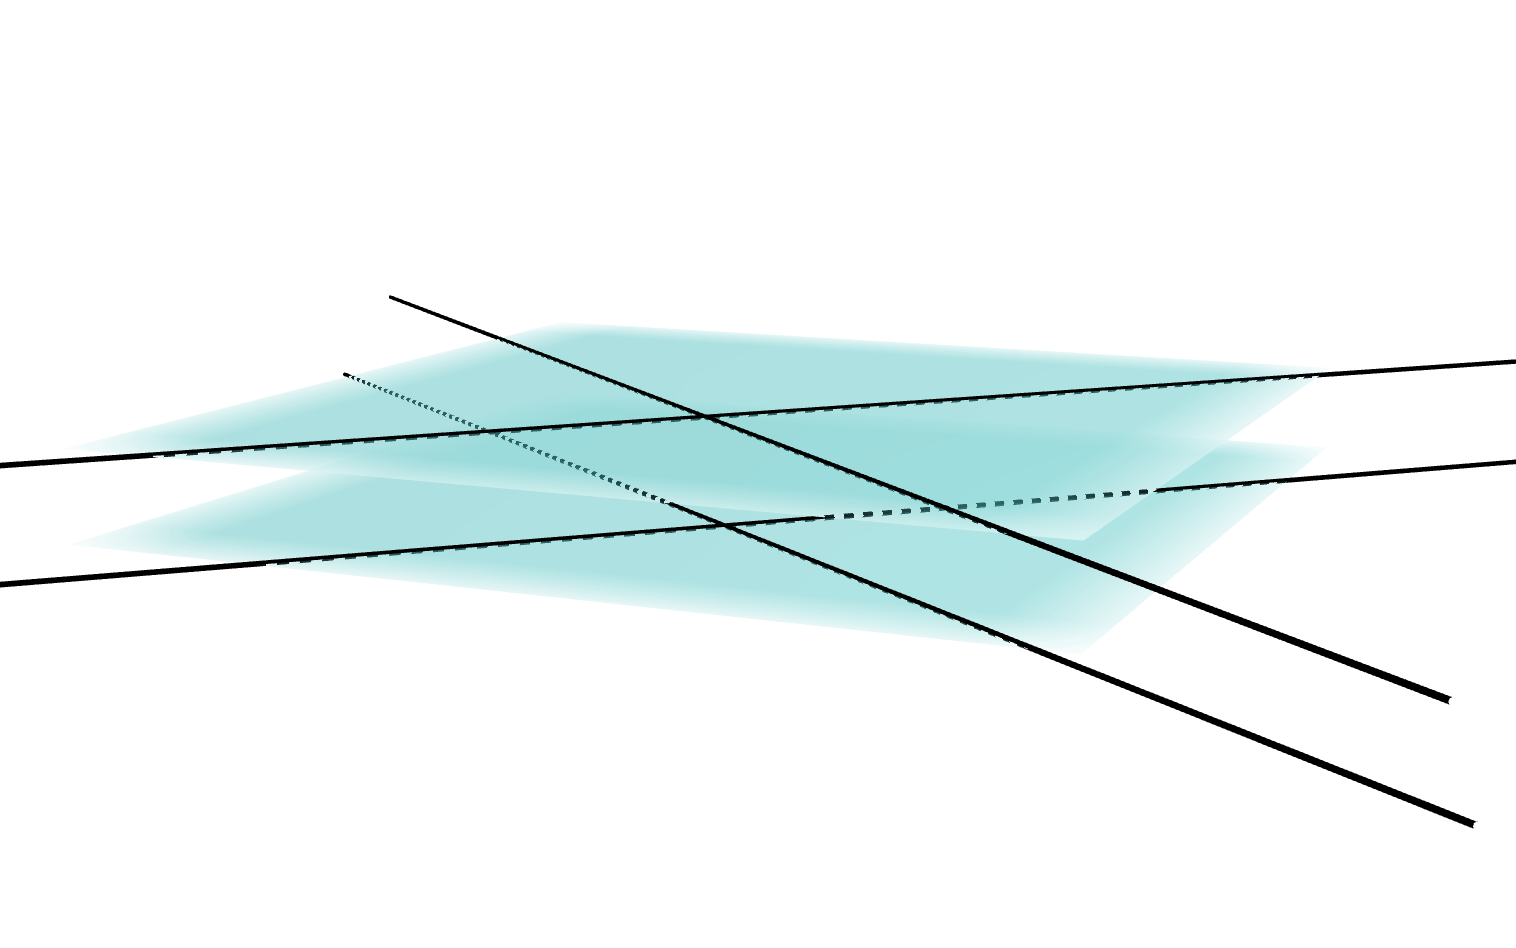
\includegraphics[width=5cm]{rsc/11fig2.png}
                    \parbox{\linewidth}{\captionof{figure}{\centering Illustration de la Propriété}}
                \end{center}
            \end{SSpartie}
            \begin{SSpartie}{Propriété} 
                Si deux plans sont parallèles, tout plan sécant à l'un est sécant à l'autre et les droites d'intersection sont parallèles.
                \begin{center}
                        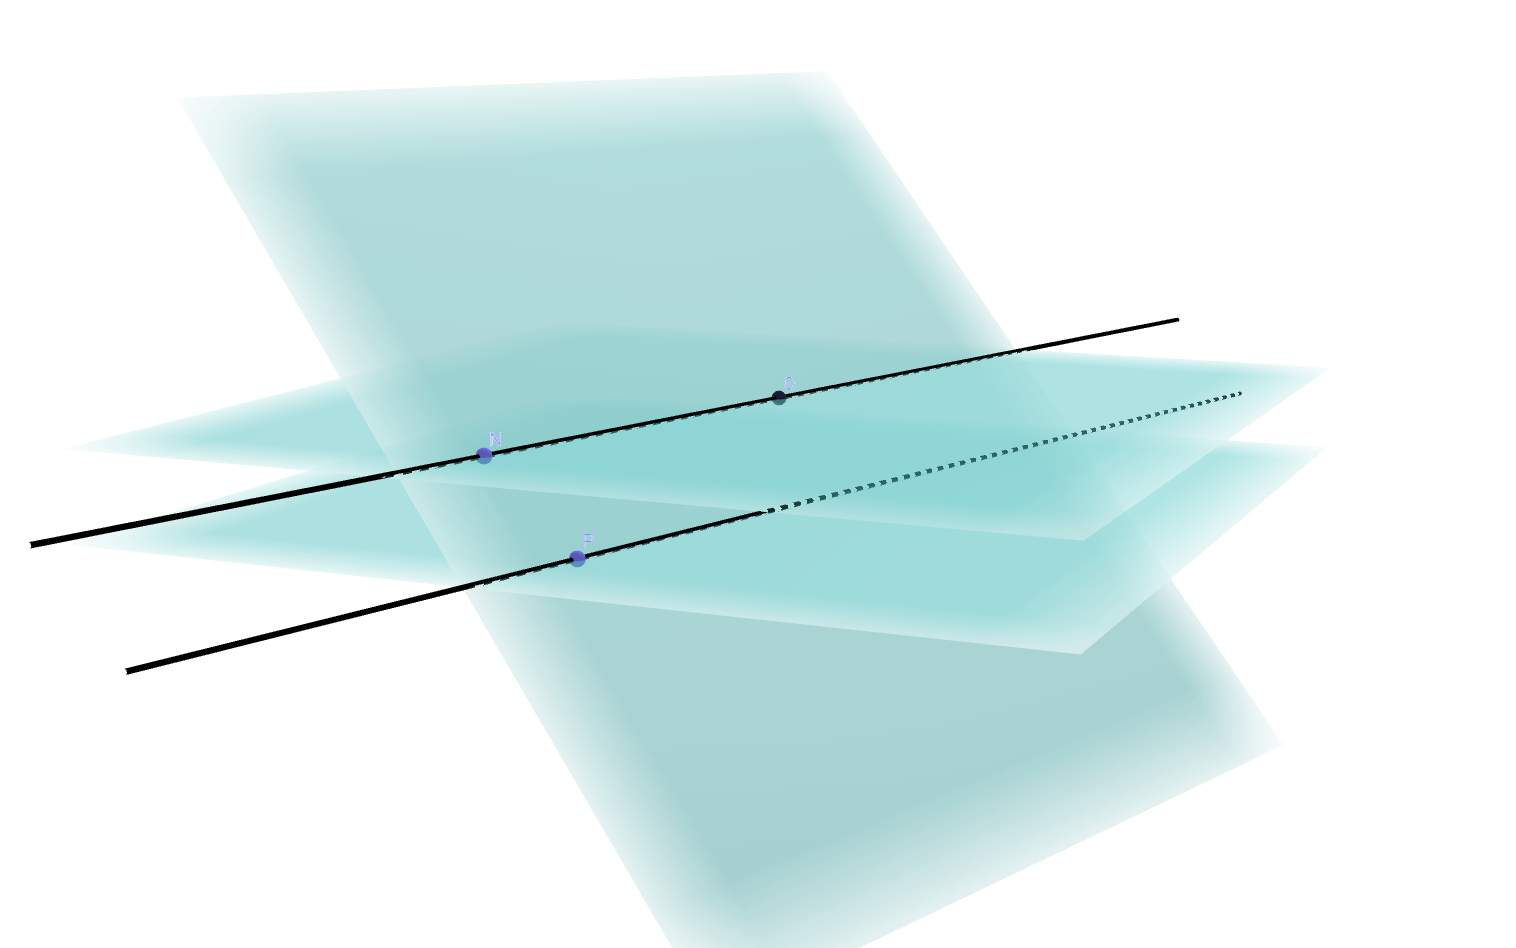
\includegraphics[width=5cm]{rsc/11fig3.png}
                    \parbox{\linewidth}{\captionof{figure}{\centering Illustration de la Propriété}}
                \end{center}
            \end{SSpartie}
            \begin{SSpartie}{Théorème dit ``du Toit''} 
                Si deux plans sécants $\mathcal{P}_1$ et $\mathcal{P}_2$ contiennent respectivement deux droites $d_1$ et $d_2$ parallèles, alors la droite d'intersection de $\mathcal{P}_1$ et $\mathcal{P}_2$ est parallèle à $d_1$ et $d_2$.
                \begin{center}
                        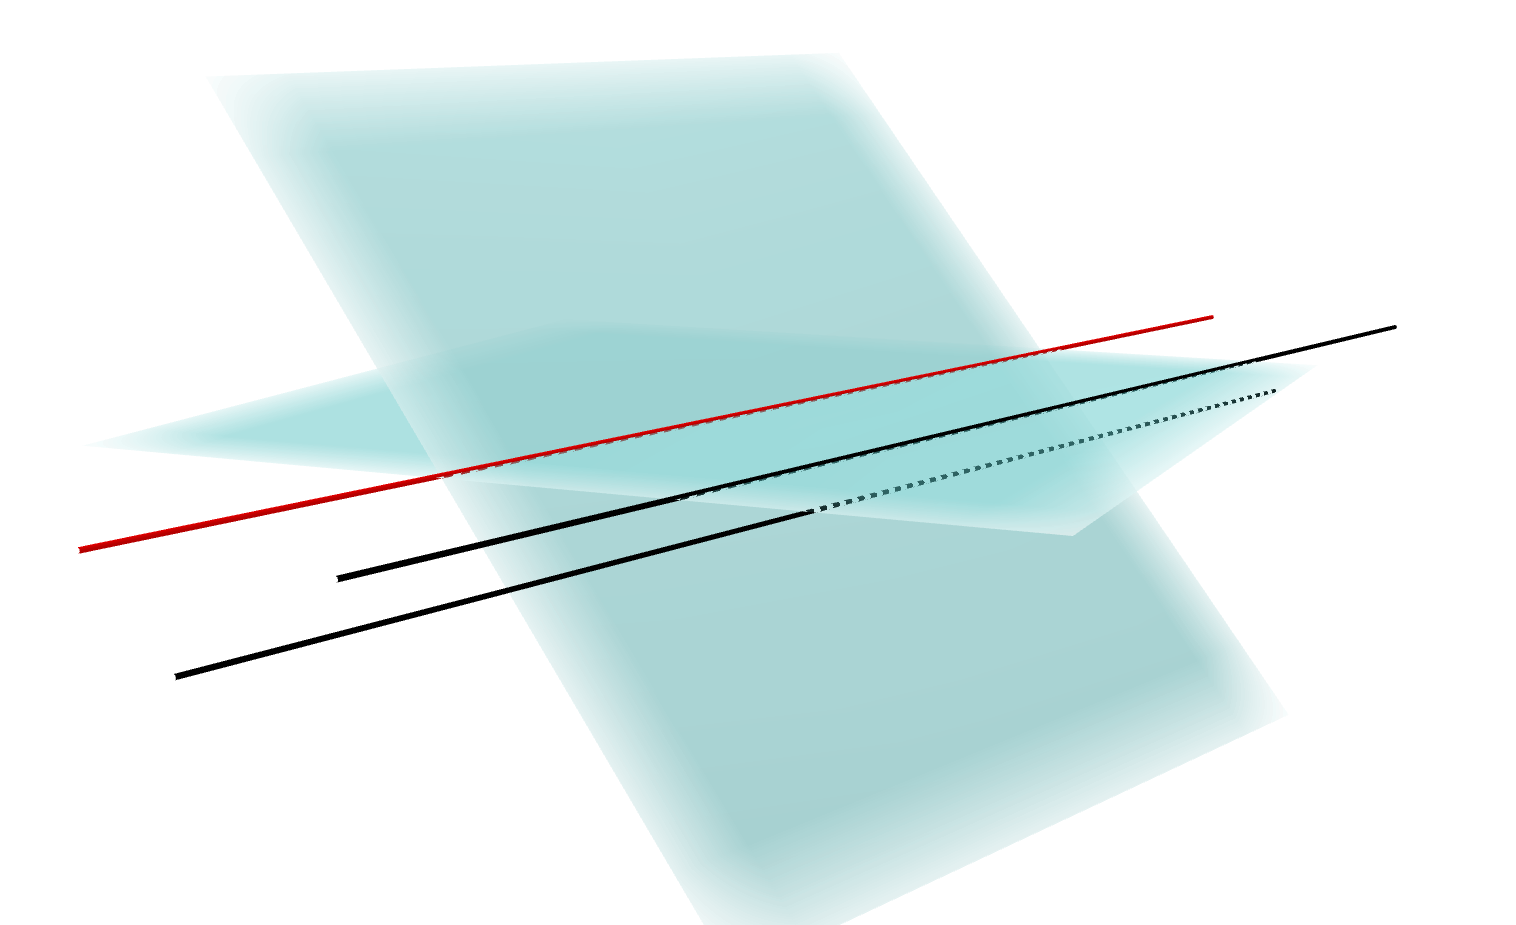
\includegraphics[width=5cm]{rsc/11fig4.png}
                    \parbox{\linewidth}{\captionof{figure}{\centering Illustration du Théorème}}
                \end{center}
            \end{SSpartie}
        \end{Spartie}
        \begin{Spartie}{Positions Relatives d'une Droite et un Plan} 
            Une droite non parallèle à un plan est sécante à ce plan. Leur intersection est un~\emph{point}.
            \begin{center}
                \begin{minipage}{4cm}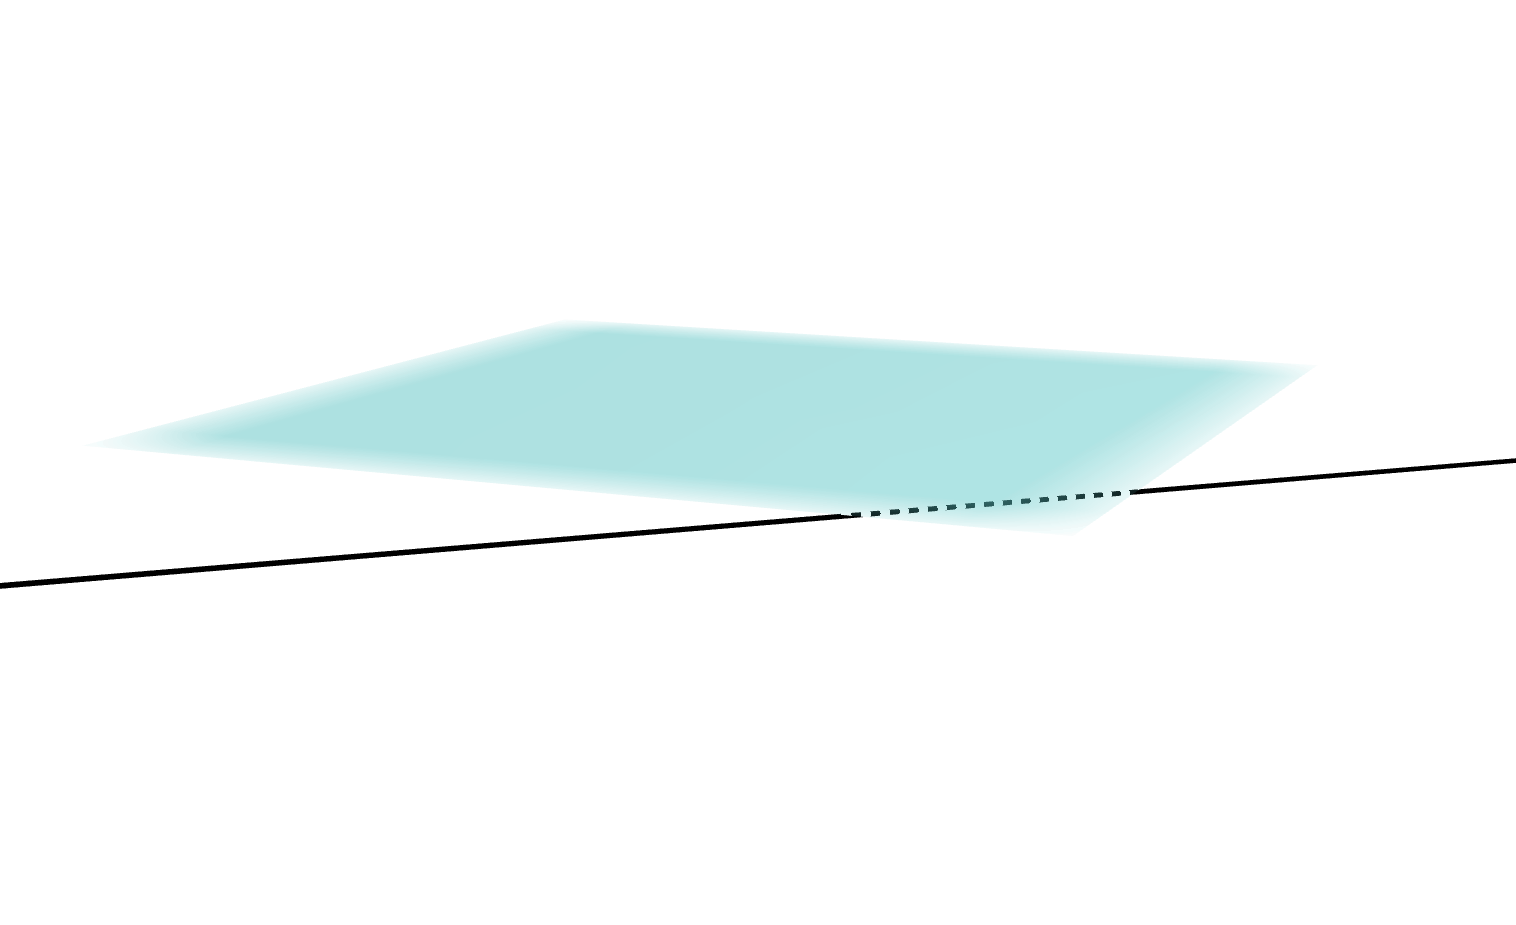
\includegraphics[width=4cm]{rsc/11fig5b.png}\\ \centering Droite strictement parallèle à un plan\end{minipage} % order of figures (b a c) intentional
                \begin{minipage}{4cm}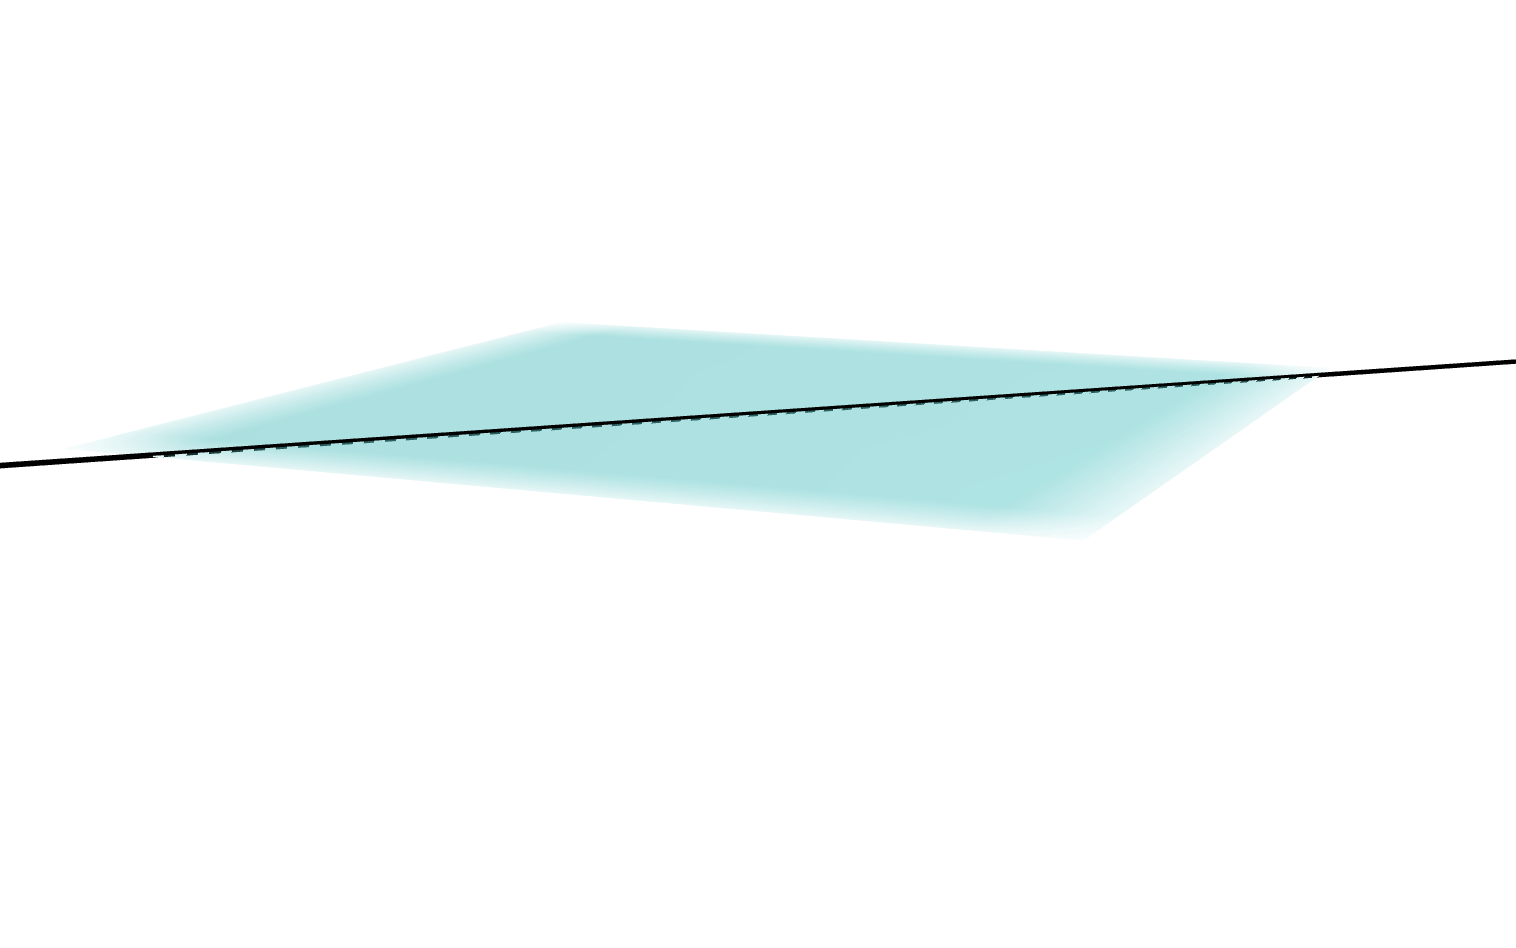
\includegraphics[width=4cm]{rsc/11fig5a.png}\\ \centering Droite incluse dans \\ un plan\end{minipage} 
                \begin{minipage}{4cm}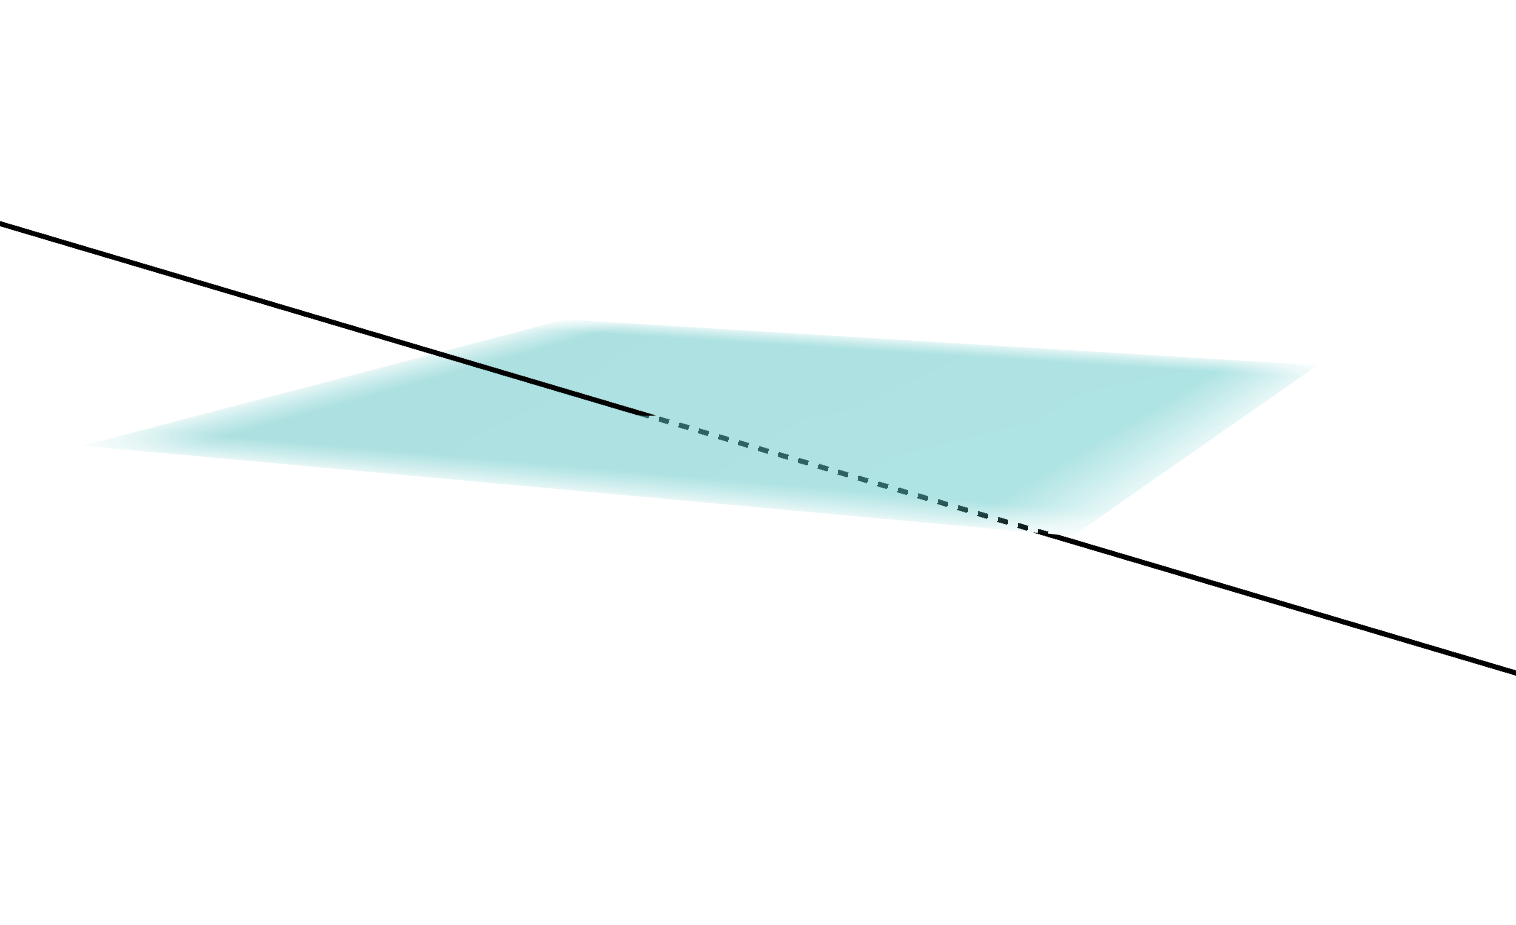
\includegraphics[width=4cm]{rsc/11fig5c.png}\\ \centering Droite sécante à un plan \end{minipage} \\[2ex]
                    C'est deux droites parallèles à un plan\hspace{4cm}\phantom{a} %shift text to left two only                
                \parbox{\linewidth}{\captionof{figure}{\centering Illustration des Positions Relatives d'un Plan et une Droite}}
            \end{center}
            \begin{SSpartie}{Propriété} 
                Une droite est parallèle à un plan si et seulement si elle est parallèle à une droite de ce plan.
            \end{SSpartie}
        \end{Spartie}
        \begin{Spartie}{Position Relative de Deux Droites} 
            \begin{SSpartie}{Définition} 
                Deux droites sont coplanaires si elles appartiennent à un même plan.
            \end{SSpartie}
            \begin{SSpartie}{Propriété} 
                Deux droites sont coplanaires si et seulement si elles sont sécantes ou parallèles.
                \begin{center}
                    \begin{minipage}{4cm}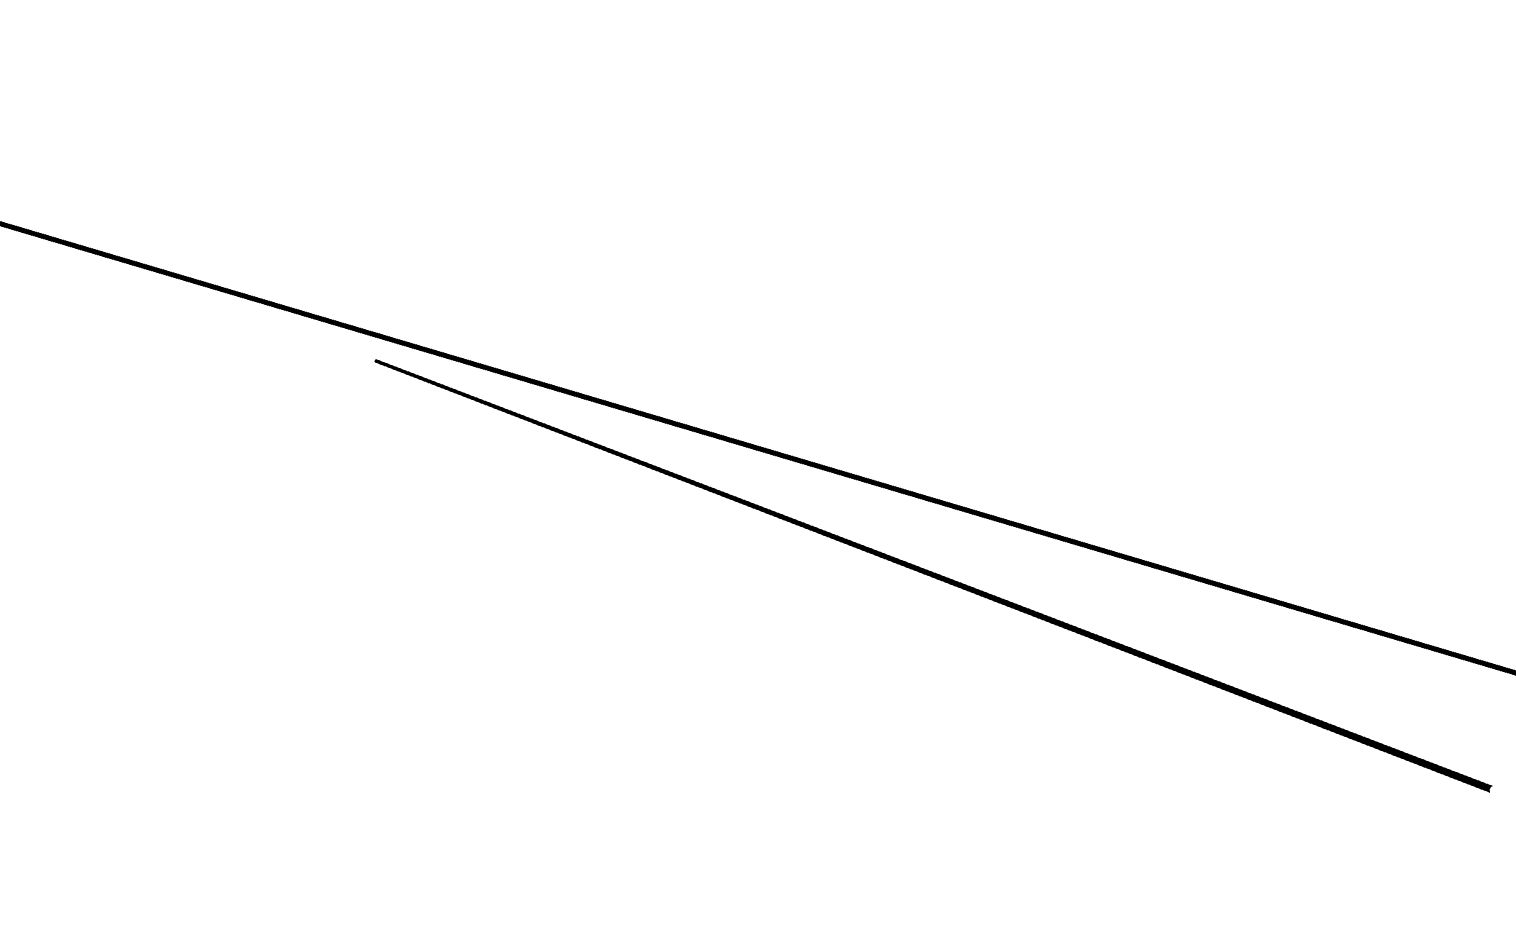
\includegraphics[width=4cm]{rsc/11fig6a.png}\\ \centering Droites non coplanaires\end{minipage}
                    \begin{minipage}{4cm}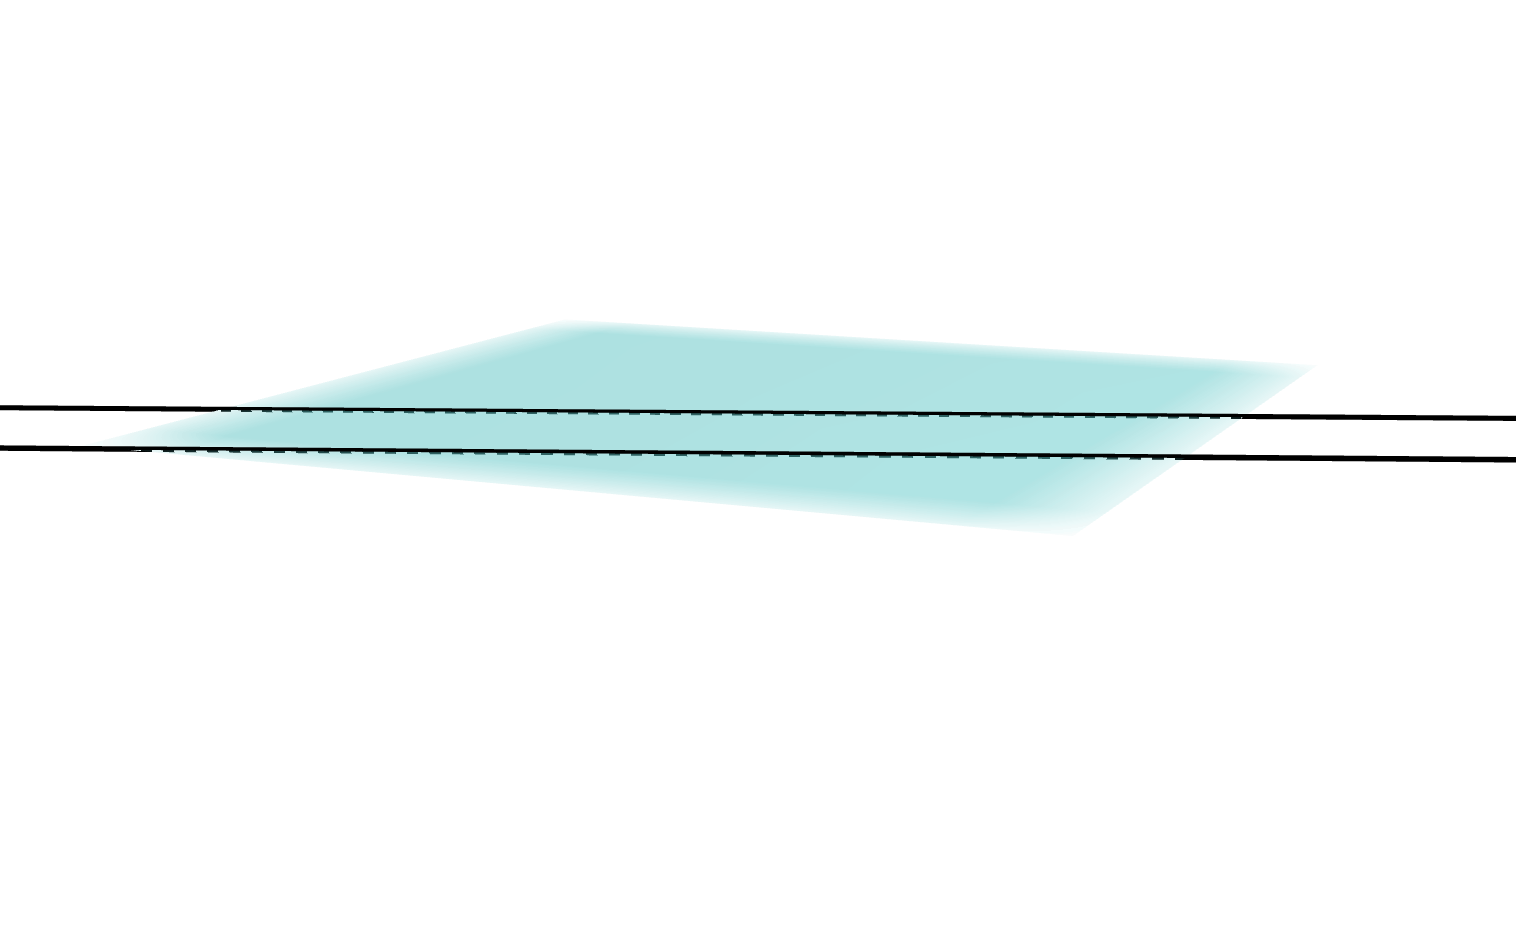
\includegraphics[width=4cm]{rsc/11fig6b.png}\\ \centering Droites strictement parallèles\end{minipage} 
                    \begin{minipage}{4cm}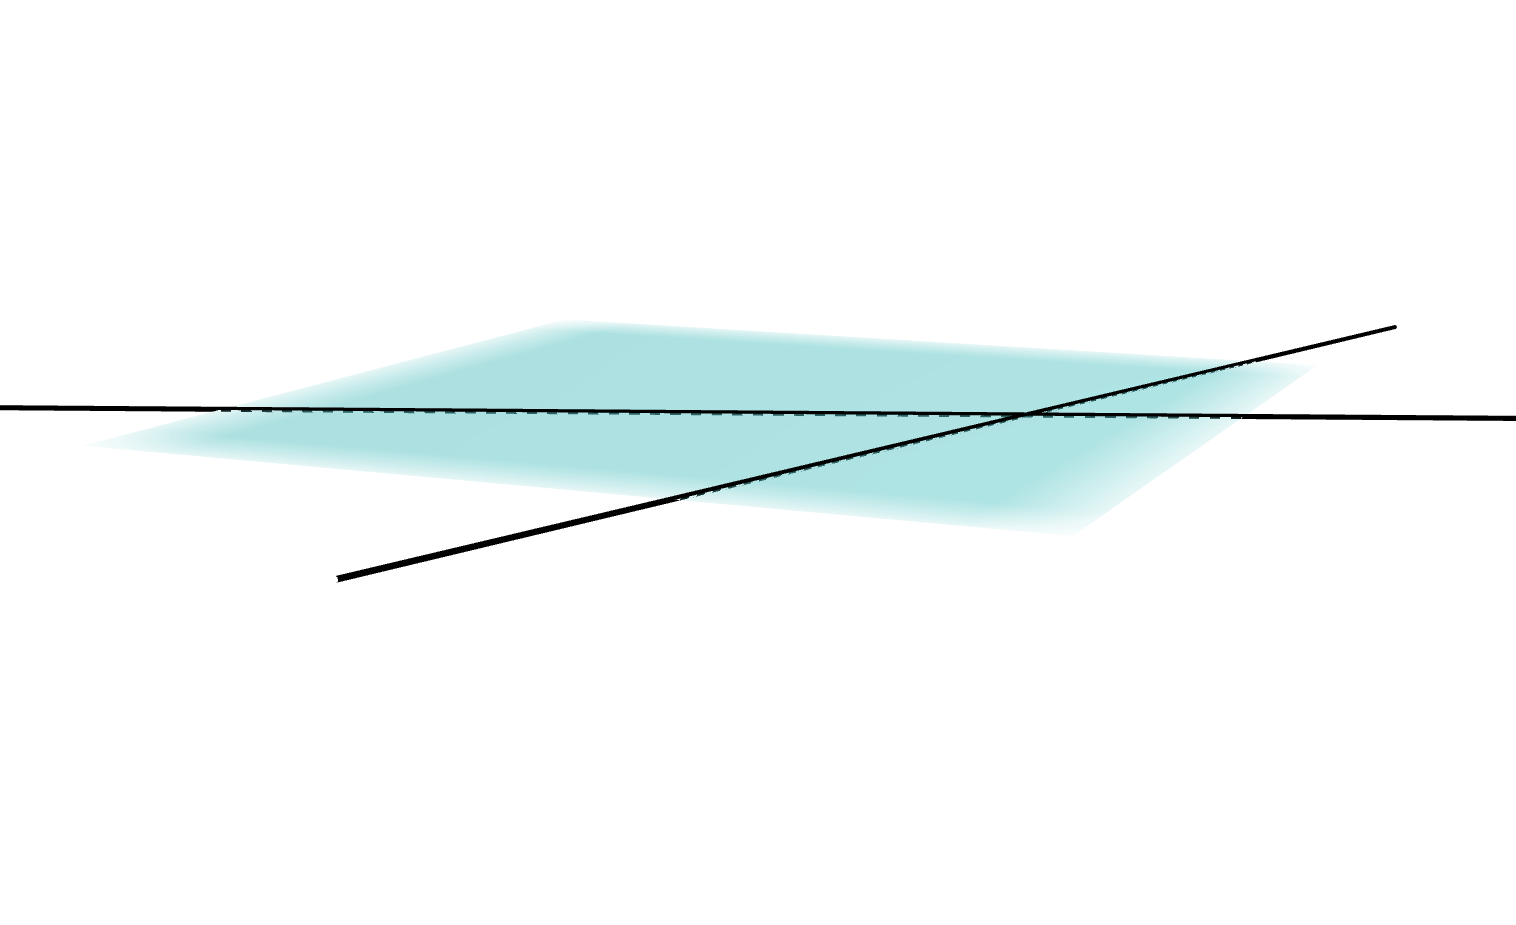
\includegraphics[width=4cm]{rsc/11fig6c.png}\\ \centering Droites sécantes\end{minipage}
                    \parbox{\linewidth}{\captionof{figure}{\centering Illustration de la Propriété}}
                \end{center}
            \end{SSpartie}
            \begin{SSpartie}{Remarque} 
                Deux droites confondues sont parallèles (au sens large)
            \end{SSpartie}
            \begin{SSpartie}{Remarque} 
                En général, deux droites de l'espace sont non coplanaires.
            \end{SSpartie}
        \end{Spartie}
    \end{Gpartie}










    
    \chapter{Orthogonalité dans l'Espace}
    
    \begin{Gpartie}{Différentes Expressions du Produit Scalaire} 
        \begin{Spartie}{Définitions} 
            $\vec{u}$ et $\vec{v}$ étant deux vecteurs de l'espace, soit un point $A$ de l'espace, et les points $B$ et $C$ tels que $\overrightarrow{AB}=\vec{u}$ et $\overrightarrow{AC}=\vec{v}$.

            Alors, $\vec{u}\cdot\vec{v}=\overrightarrow{AB}\cdot\overrightarrow{AC}$\quad(Produit Scalaire de deux vecteurs dans le plan (ABC))

            Ainsi, toutes les définitions et propriétés du produit scalaire dans le plan sont conservées dans l'espace.

            Les trois définitions suivantes sont équivalentes :
            \begin{SSpartie}{Définition avec le Projeté Orthogonal} 
                $\vec{u}$ et $\vec{v}$ étant deux vecteurs de l'espace, soit un point $A$ de l'espace, et les points $B$ et $C$ tels que $\overrightarrow{AB}=\vec{u}$ et $\overrightarrow{AC}=\vec{v}$.

                Soit $H$ le projeté orthogonal de $C$ sur $(AB)$,

                $\overrightarrow{AB}\cdot\overrightarrow{AC}=AB\times AH$ si $\overrightarrow{AB}$ et $\overrightarrow{AH}$ sont de même sens. \\
                $\overrightarrow{AB}\cdot\overrightarrow{AC}=-AB\times AH$ si $\overrightarrow{AB}$ et $\overrightarrow{AH}$ sont de sens contraire.
                \begin{center}
                    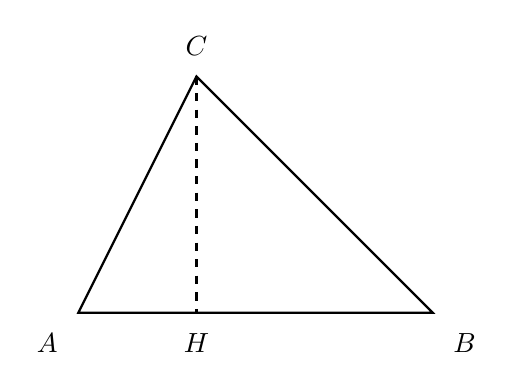
\begin{tikzpicture}[scale=3]
                        \coordinate (A) at (-0.5,0);
                        \coordinate (B) at (1,0);
                        \coordinate (C) at (0,1);
                        \coordinate (H) at (0,0);
                        \draw[thick]  (A) node[label=below left:$A$] {} -- (H) -- (B) node[label=below right:$B$] {} --  (C) node[label=above:$C$] {} -- cycle;
                        \draw[thick, dashed] (C) -- (H) node[label=below:$H$] {};
                    \end{tikzpicture}\hspace{2cm}
                    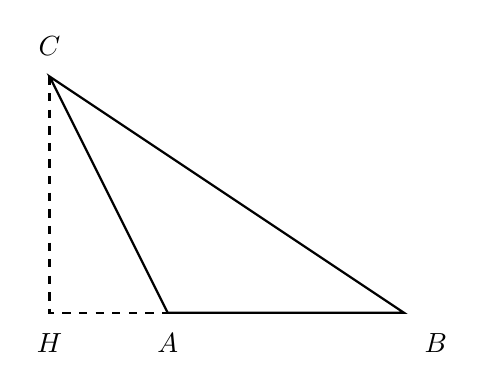
\begin{tikzpicture}[scale=3]
                        \coordinate (A) at (0.5,0);
                        \coordinate (B) at (1.5,0);
                        \coordinate (C) at (0,1);
                        \coordinate (H) at (0,0);
                        \draw[thick] (A) node[label=below:$A$] {} -- (B) node[label=below right:$B$] {} -- (C) -- cycle;
                        \draw[dashed, thick] (C) node[label=above:$C$] {} -- (H) node[label=below:$H$] {} -- (A);
                    \end{tikzpicture}
                    \[\overrightarrow{AB}\cdot\overrightarrow{AC}=\overrightarrow{AB}\cdot\overrightarrow{AH}\]\[=AB\times AH\qquad\text{ou}\qquad=-AB\times AH\]
                    \parbox{\linewidth}{\captionof{figure}{\centering Illustration du Produit Scalaire par Projeté Orthogonal}}
                \end{center}
            \end{SSpartie}
            \begin{SSpartie}{Définitions avec les Normes} 
                $\vec{u}\cdot\vec{v}=\dfrac{1}{2}\left(\lvert\lvert\vec{u}+\vec{v}\rvert\rvert^2-\lvert\lvert\vec{u}\rvert\rvert^2-\lvert\lvert\vec{v}\rvert\rvert^2\right)=\dfrac{1}{2}\left(\lvert\lvert\vec{u}\rvert\rvert^2+\lvert\lvert\vec{v}\rvert\rvert^2-\lvert\lvert\vec{u}-\vec{v}\rvert\rvert^2\right)$

                Ainsi, $\overrightarrow{AB}\cdot\overrightarrow{AC}=\dfrac{1}{2}\left(AB^2+AC^2-CB^2\right)$.
            \end{SSpartie}
            \begin{SSpartie}{Définition avec l'Angle} 
                $\vec{u}\cdot\vec{v}=\lvert\lvert\vec{u}\rvert\rvert\times\lvert\lvert\vec{v}\rvert\rvert\times\cos\,\left(\vec{u}~,\vec{v}\right)$
            \end{SSpartie}
        \end{Spartie}
        \begin{Spartie}{Propriétés} 
            Pour tous vecteurs $\vec{u}$, $\vec{v}$ et $\vec{w}$, et pour tout réel $\lambda$ : \[\vec{u}\cdot\vec{v}=\vec{v}\cdot\vec{u}\qquad\text{(symmétrie du produit scalaire)}\] \[\begin{drcases}\left(\lambda\vec{u}\right)\cdot\vec{v}=\lambda\times\left(\vec{u}\cdot\vec{v}\right)=\vec{u}\cdot\left(\lambda\vec{v}\right) \\ \vec{u}\cdot\left(\vec{v}+\vec{w}\right)=\vec{u}\cdot\vec{v}+\vec{u}\cdot\vec{w}\end{drcases}\text{(bilinéarité du produit scalaire)}\]
        \end{Spartie}
        \begin{Spartie}{Expressions Analytique du Produit Scalaire} 
            Dans un repère orthonormé de l'espace, $\vec{u}~\left(x~;y~;z\right)$ et $\vec{v}~\left(x'~;y'~;z'\right)$ étant deux vecteurs, alors : \[\vec{u}\cdot\vec{v}=xx'+yy'+zz'\] 
            \begin{SSpartie}{Démonstration} 
                On rappelle que $\lvert\lvert\vec{u}\rvert\rvert=\sqrt{x^2+y^2+z^2}$ :

                $\begin{aligned}[t]
                    \vec{u}\cdot\vec{v}&=\dfrac{1}{2}\left(\lvert\lvert\vec{u}+\vec{v}\rvert\rvert^2-\lvert\lvert\vec{u}\rvert\rvert^2-\lvert\lvert\vec{v}\rvert\rvert^2\right) \\
                    &=\frac{1}{2}\left(\left(x+x'\right)^2+\left(y+y'\right)^2+\left(z+z'\right)^2-\left(x^2+y^2+z^2\right)-\left(x'^2+y'^2+z'^2\right)\right) \\
                    &=\frac{1}{2}\left(2xx'+2yy'+2zz'\right) \\
                    &=xx'+y y'+z z'
                \end{aligned}$
            \end{SSpartie}
        \end{Spartie}
    \end{Gpartie}
    \begin{Gpartie}{Orthogonalité} 
        \begin{Spartie}{Vecteurs Orthogonaux} 
            \begin{SSpartie}{Définition} 
                Deux vecteurs de l'espace non nuls sont orthogonaux si deux droites qu'ils dirigent sont orthogonales.

                Par convention le vecteur nul est orthogonal à tout vecteur.
                \pagebreak
                \begin{SSSpartie}{Exemple} 
                    $\vec{u}$ et $\vec{v}$ sont orthogonaux.

                    \begin{center}
                            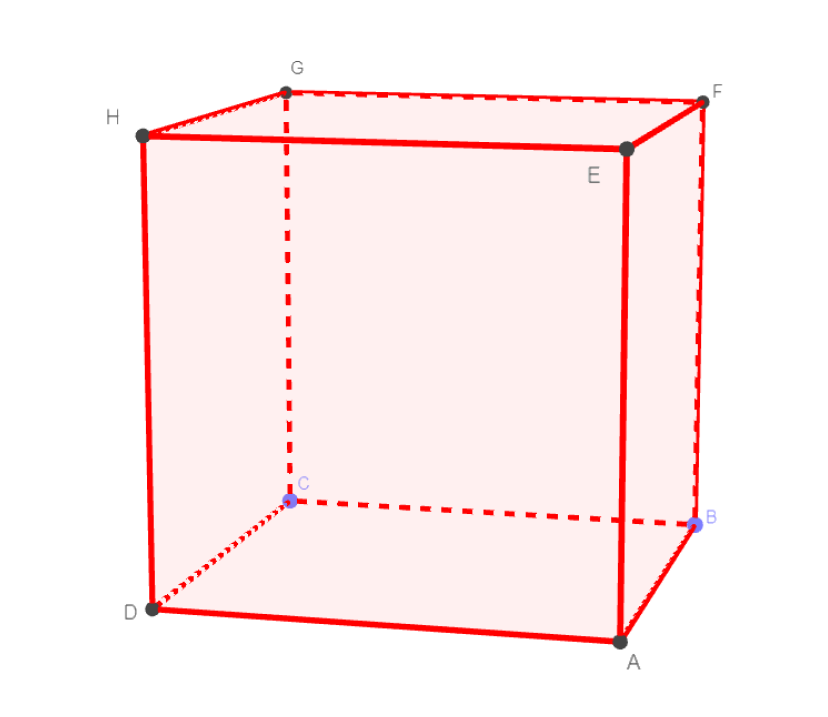
\includegraphics[width=5cm]{rsc/12fig2.png}
                            \[\overrightarrow{AB}\quad\text{et}\quad\overrightarrow{DC}\quad\text{sont orthogonaux.}\]
                        \parbox{\linewidth}{\captionof{figure}{\centering Illustration de deux Vecteurs Orthogonaux}}
                    \end{center}
                \end{SSSpartie}
            \end{SSpartie}
            \begin{SSpartie}{Théorème} 
                Deux vecteurs $\vec{u}$ et $\vec{v}$ sont orthogonaux si et seulement si $\vec{u}\cdot\vec{v}=0$.
            \end{SSpartie}
            \begin{SSpartie}{Théorème} 
                Dans un repère orthonormé, deux vecteurs $\vec{u}~\left(x~;y~;z\right)$ et $\vec{v}~\left(x'~;y'~;z'\right)$ sont orthogonaux si et seulement si $xx'+yy'+zz'=0$ (par définition analytique)
            \end{SSpartie}
        \end{Spartie}
        \begin{Spartie}{Vecteur Normal à un Plan} 
            \begin{SSpartie}{Définition} 
                Un vecteur \emph{normal} à un plan est un vecteur directeur d'une droite orthogonale à un plan.
    
                Un vecteur normal est par définition \emph{non nul}.
    
                \begin{center}
                        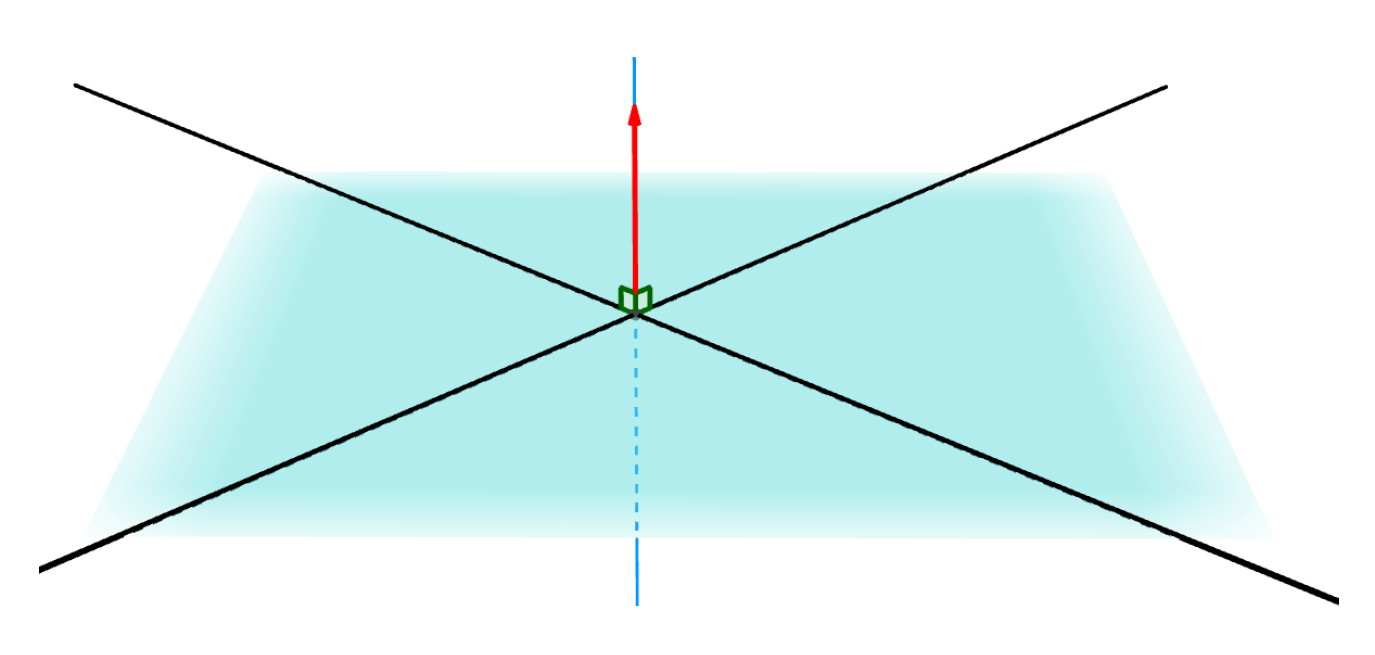
\includegraphics[width=5cm]{rsc/12fig3.png}
                    \parbox{\linewidth}{\captionof{figure}{\centering Illustration de la Définition}}
                \end{center}
            \end{SSpartie}
            \pagebreak
            \begin{SSpartie}{Caractérisation d'un Plan}
                Un plan est caractérisé par \emph{un point} et un \emph{vecteur normal}.

                \begin{center}
                    
\includegraphics[width=5cm]{rsc/12fig4.png}
                    \parbox{\linewidth}{\captionof{figure}{\centering Caractérisation d'un Plan}}
                \end{center}
                
                                    Sur ce dessin, les deux plans ont le meme vecteur normal $\vec{n}$, donc la meme direction. La position d'un plan sera déterminée par un point.
                
                                    On en déduit que deux plans parallèles admettent le meme vecteur normal, c'est-à-dire des vecteurs normaux colinéaires.
                \begin{SSSpartie}{Rappel} 
                    On peut aussi définir un plan par trois points non alignés, ou par deux droites sécantes (c'est-à-dire un point et deux vecteurs directeurs), ou, beaucoup plus rare, par deux droites parallèles non confondues.
                \end{SSSpartie}
            \end{SSpartie}
            \begin{SSpartie}{Théorème} 
                Le plan $\mathcal{P}$ qui passe par un point $A$ et de vecteur normal $\vec{n}$ est l'ensemble des point $M$ tels que $\overrightarrow{AM}\cdot\vec{n}=0$.\quad (admis ou définition d'un plan)

                \begin{center}
                    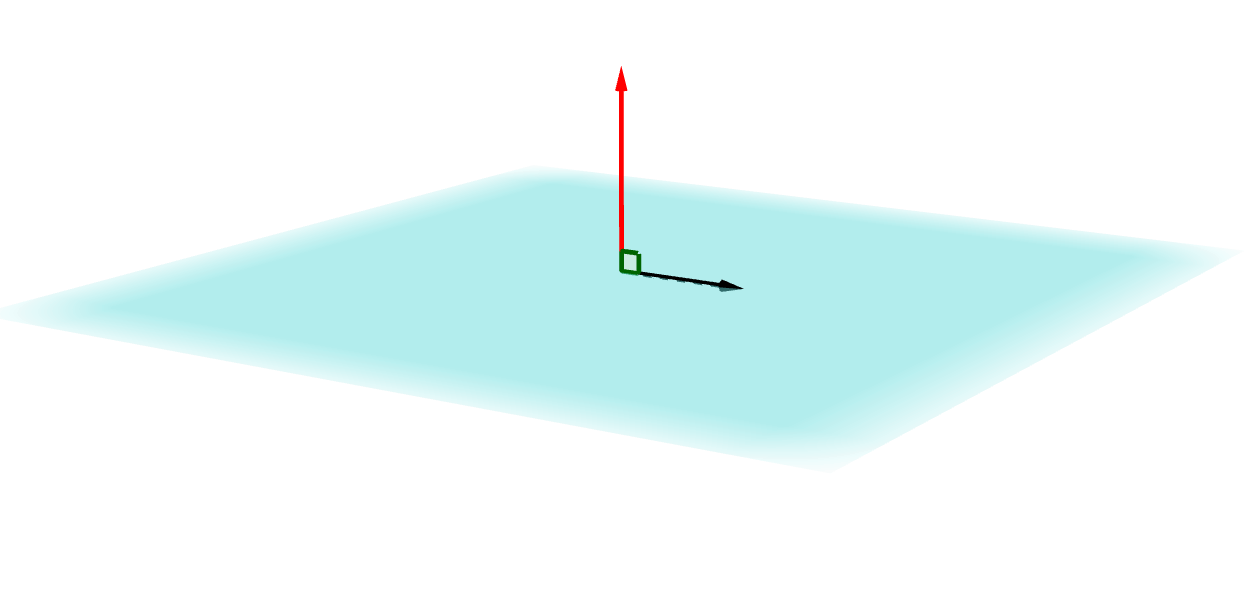
\includegraphics[width=5cm]{rsc/12fig5.png}
                    \parbox{\linewidth}{\captionof{figure}{\centering Illustration du Théorème}}
                \end{center}
            \end{SSpartie}
        \end{Spartie}
        \begin{Spartie}{Application (approfondissement)} 
            \begin{SSpartie}{Démonstration du Théorème} 
                \og Une droite est orthogonale à un plan si et seulement si elle est orthogonale à deux droites sécantes de ce plan. \fg
                \begin{itemize}[leftmargin=7ex]
                    \item[``$\implies$''] Si une droite est orthogonale à un plan, elle est orthogonale à toute droite de ce plan, en particulier deux droites sécantes de ce plan.
                    \item[``$\impliedby$''] Supposons qu'une droite $(d)$ est orthogonale à deux droites sécantes $d_1$ et $d_2$ du plan $\mathcal{P}$. Notons $A$ le point d'intersection de $d_1$ et $d_2$, et $\vec{u_1}$ et $\vec{u_2}$ deux vecteurs directeurs de $d_1$ et $d_2$.

                    Ainsi $\left(~A~;~\vec{u_1}~,~\vec{u_2}~\right)$ est un repère du plan $\mathcal{P}$, car $\vec{u_1}$ et $\vec{u_2}$ ne sont pas colinéaires.

                    Notons $\vec{n}$ un vecteur directeur de $(d)$. (on trace ci-dessous uniquement les vecteurs directeurs)
                    \vspace{-0.2ex}
                    \begin{center}
                        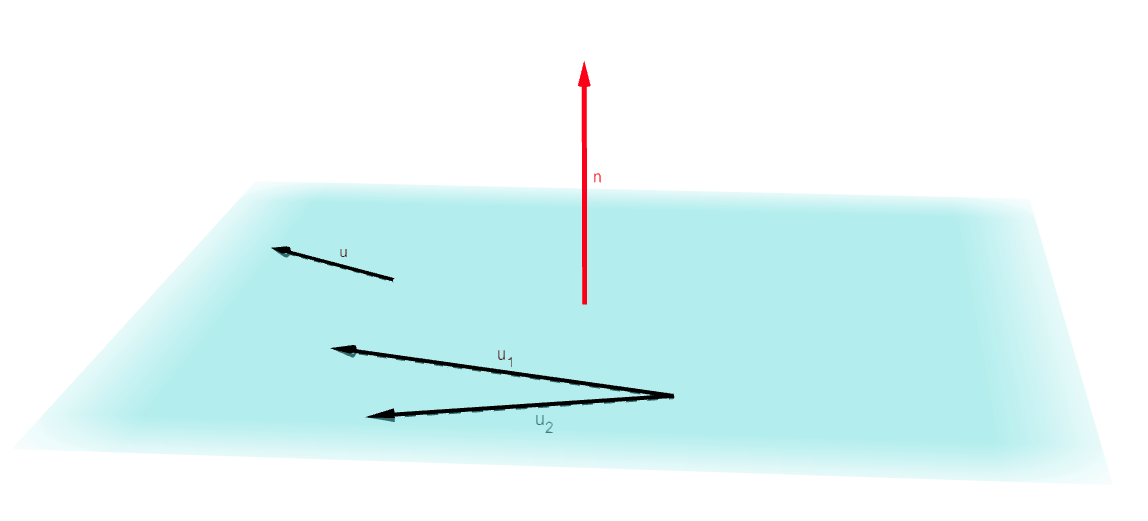
\includegraphics[width=5cm]{rsc/12fig6.png}
                        \parbox{\linewidth}{\captionof{figure}{\centering Représentation de la Situation}}
                    \end{center}
    
                    Alors, $\vec{n}$ est orthogonal à $\vec{u_1}$ et $\vec{u_2}$.

                    Soit une droite du plan $\mathcal{P}$, dont le vecteur directeur est $\vec{u}$.

                    Alors, il existe deux réels $\alpha$ et $\beta$ tels que $\vec{u}=\alpha\vec{u_1}+\beta\vec{u_2}$~($\vec{u}$, $\vec{u_1}$, $\vec{u_2}$ coplanaires)

                    Donc, $\vec{n}\cdot\vec{u}=\alpha\vec{n}\cdot\vec{u_1}+\beta\vec{n}\cdot\vec{u_2}=0$\quad (car $\vec{n}$ orthogonal à $\vec{u_1}$ et $\vec{u_2}$)

                    Ainsi, $\vec{n}$ est orthogonal à $\vec{u}$, et donc $(d)$ est orthogonale à toute droite du plan~$\mathcal{P}$.\quad$\square$
                \end{itemize}
            \end{SSpartie}
        \end{Spartie}
        \begin{Spartie}{Plans Perpendiculaires} 
            Deux plans $\mathcal{P}_1$ et $\mathcal{P}_2$ admettant pour vecteurs normaux respectivement $\vec{n_1}$ et $\vec{n_2}$ sont perpendiculaires si et seulement si $\vec{n_1}\cdot\vec{n_2}=0$.

            \begin{center}
                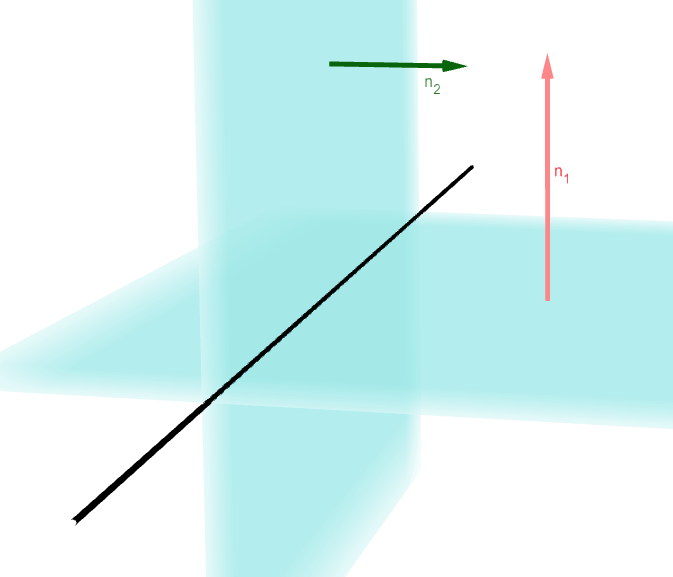
\includegraphics[width=5cm]{rsc/12fig7.png}
                \parbox{\linewidth}{\captionof{figure}{\centering Illustration de deux Plans Perpendiculaires}}
            \end{center}
        \end{Spartie}
    \end{Gpartie}
    \vfill\pagebreak
    \begin{Gpartie}{Projection Orthogonale d'un Point} 
        \begin{Spartie}{Projeté Orthogonal d'un Point sur un Plan} 
            \begin{SSSpartie}{Définition} 
                Le projeté orthogonal d'un point $A$ sur un plan $\mathcal{P}$ est l'intersection de $\mathcal{P}$ et de la droite orthogonale à $\mathcal{P}$ passant par $A$.
            \end{SSSpartie}
            \begin{SSSpartie}{Remarque} 
                Il existe une unique droite orthogonale (perpendiculaire) à $\mathcal{P}$ passant par $A$.
            \end{SSSpartie}
            \begin{SSSpartie}{Propriété} 
                Si $H$ est le projeté orthogonal du point $A$ sur le plan $\mathcal{P}$, le point $H$ est le point de $\mathcal{P}$ le plus proche de $A$. On l'appelle distance du point $A$ au plan $\mathcal{P}$.
                
                \begin{center}
                    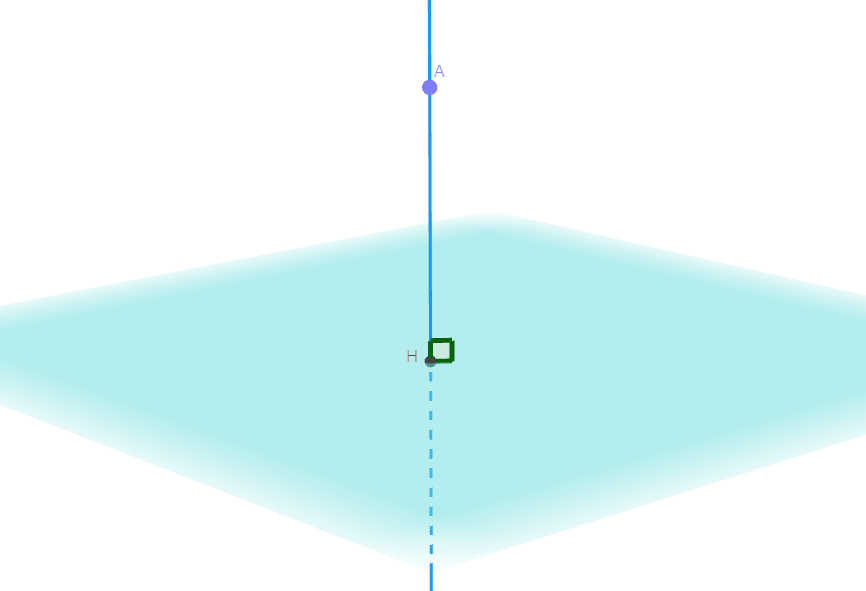
\includegraphics[width=5cm]{rsc/12fig8.png}
                    \parbox{\linewidth}{\captionof{figure}{\centering Illustration de la Propriété}}
                \end{center}

                \begin{SSSSpartie}{Démonstration} 
                    Soit $M$ un point de $\mathcal{P}$, comme $(AH)\perp\mathcal{P},~(AH)$ est orthogonale à toute droite de ce plan. \\ Donc $AMH$ est un triangle rectangle en $H$ et $AH^2=AM^2-MH^2\leq AM^2$

                    Donc, pour tout point $M$ du plan, $AH\leq AM$.

                    \begin{center}
                        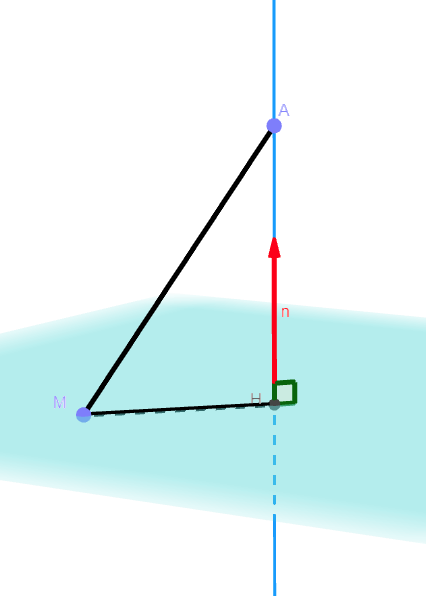
\includegraphics[width=5cm]{rsc/12fig9.png}
                        \parbox{\linewidth}{\captionof{figure}{\centering Illustration de la Démonstration}}
                    \end{center}    
                \end{SSSSpartie}
            \end{SSSpartie}
            \begin{SSSpartie}{Propriété} 
                Pour tout point $M$ du plan $\mathcal{P}$ : \[AH=\frac{\left\lvert\overrightarrow{AM}\cdot\vec{n}\right\rvert}{\lvert\lvert\vec{n}\rvert\rvert}=d~\left(~A~,~\mathcal{P}~\right)\]
                \begin{SSSSpartie}{Démonstration} 
                    $AH=AM\times\cos\,\left(~\widehat{MAH}~\right)$\quad (triangle rectangle AMH)

                    Or $\overrightarrow{AM}\cdot\vec{n}=AM\times\lvert\lvert\vec{n}\rvert\rvert\times\cos\,\left(~\overrightarrow{AM}~,~\vec{n}~\right)$

                    Donc $\left\lvert\overrightarrow{AM}\cdot\vec{n}\right\rvert=AM\times\lvert\lvert\vec{n}\rvert\rvert\times\left\lvert\cos\,\left(~\overrightarrow{AM}~,~\vec{n}~\right)\right\rvert=AM\times\lvert\lvert\vec{n}\rvert\rvert\times\cos\,\left(~\widehat{MAH}~\right)$

                    Et donc, $\dfrac{\left\lvert\overrightarrow{AM}\cdot\vec{n}\right\rvert}{\lvert\lvert\vec{n}\rvert\rvert}=AH$
                \end{SSSSpartie}
            \end{SSSpartie}
        \end{Spartie}
        \begin{Spartie}{Projeté Orthogonal d'un Point sur une Droite} 
            \begin{SSpartie}{Définition} 
                Le projeté orthogonal d'un point $A$ sur une droite $(d)$ est l'intersection de $(d)$ et du plan orthogonal à $(d)$ passant par $A$.
            \end{SSpartie}
            \begin{SSpartie}{Remarque} 
                Il existe un unique plan orthogonal (perpendiculaire) à $(d)$ passant par $A$.
            \end{SSpartie}
            \begin{SSpartie}{Propriété} 
                Si $H$ est le projeté orthogonal du point $A$ sur la droite $(d)$, le point $H$ est le point de $(d)$ le plus proche de $A$. On l'appelle distance du point $A$ à la droite $(d)$.
            \end{SSpartie}
        \end{Spartie}
    \end{Gpartie}






    \chapter{Équations dans l'Espace}

    
    \begin{Gpartie}{Représentation Paramétrique d'une Droite} 
        Dans un repère $\left(O~;\vec{\imath}~,\vec{\jmath}~,\vec{k}\right)$, soit $(d)$ la droite passant par un point $A~\left(x_A~;y_A~;z_A\right)$ et de vecteur directeur $\vec{u}~\big(a~;b~;c\big)$

        Un point $M~\left(x~;y~;z\right)$ appartient à $(d)$ si et seulement si il existe un réel $t$ tel que $\overrightarrow{AM}=t\vec{u}$

        C'est-à-dire : $(S)\begin{cases} x=x_A+ta \\ y=y_A+tb \\ z=z_A+tc \end{cases}\left(t\in\mathbb{R}\right)$

        \begin{Spartie}{Définition} 
            Le système $(S)$ est une représentation paramétrique de la droite $(d)$. $t$ est le paramètre de cette représentation.
            \begin{SSpartie}{Démonstration}
                Reprenons la situation précédente. 
                
                $\overrightarrow{AM}~\begin{psmallmatrix} x_M-x_A &=\ x-x_A \\ y_M-y_A &=\ y-y_A \\ z_M-z_A &=\ z-z_A \end{psmallmatrix}$

                $\begin{aligned}[t]
                    M\in(d)&\iff\overrightarrow{AM}=t\vec{u} \\
                    &\iff\begin{pmatrix} x-x_A \\ y-y_A \\ z-z_a \end{pmatrix}=t\begin{pmatrix} a \\ b \\ c \end{pmatrix} \\
                    &\iff\begin{cases}x-x_A=ta \\ y-y_A=tb \\ z-z_A= t c \end{cases} \\ %spaces to supress spellchecker
                    &\iff\begin{cases}x=x_A+ta \\ y=y_A+tb \\ z=z_A+ t c \end{cases}
                \end{aligned}$
            \end{SSpartie}
        \end{Spartie}
        \begin{Spartie}{Exemple} 
            La droite $(d)$ passant par $A~\left(~2~;0~;-1~\right)$ et de vecteur directeur $\vec{u}~\begin{psmallmatrix}1 \\ -3 \\ 2\end{psmallmatrix}$ a pour représentation paramétrique : \[(d)\begin{cases} x=2+t \\ y=-3t \\ z=-1+2t
            \end{cases}\left(t\in\mathbb{R}\right)\]

            Les points $M~\left(~0~;~6~;~-5~\right)$ et $N~\left(~1~;~3~;~2~\right)$ appartiennent-ils à $(d)$ ?
            \begin{itemize}
                \item $M$ : $\begin{cases} 0=2+t \\ 6=-3t \\ -5=-1+2t \end{cases}M\in(d)$, car $-2$ est solution du système.
                \item $N$ : $\begin{cases} 1=2+t \\ 3=-3t \\ 2=-1+2t \end{cases}N\notin(d)$, car $-1$ est solution de $(1)$ et $(2)$ mais pas $(3)$.
            \end{itemize}
        \end{Spartie}
    \end{Gpartie}
    \begin{Gpartie}{Équation Cartésienne de Plan} 
        \begin{Spartie}{Rappel} 
            La plan $\mathcal{P}$ qui passe par un point $A$ et de vecteur normal $\vec{n}$ est l'ensemble des points $M$ tels que $\overrightarrow{AM}\cdot\vec{n}=0$
        \end{Spartie}
        \begin{Spartie}{Théorème} 
            \begin{enumerate}[(1)]
                \item   L'ensemble des points $M~\left(x~;y~;z\right)$ tels que $ax+by+cz+d=0$, où $a$, $b$, $c$ et $d$ sont quatre réels tels que $a$, $b$ et $c$ sont non nuls, est un plan de vecteur normal $\vec{n}~\left(a~,b~,c\right)$.
                
                \item   Réciproquement : si $\vec{n}~\left(a~,b~,c\right)$ est un vecteur normal d'un plan $\mathcal{P}$, une équation cartésienne de ce plan est $ax+by+cz+d=0$ où $d$ est un réel.
                
                Autrement dit, pour tout point $M~\left(x~;y~;z\right)$ de $\mathcal{P}$ vérifie $ax+by+cz+d=0$
            \end{enumerate}
            \begin{SSpartie}{Démonstration} 
                \begin{enumerate}[(1)]
                    \item   Appelons $\mathcal{E}$ l'ensemble des points $M~\left(x~;y~;z\right)$ tels que $ax+by+cz+d=0$ (on ne sait pas que c'est un plan) \\ Soit le vecteur $\vec{n}~\left(a~,b~,c\right)$
                    
                    Supposons $a\neq 0$, prenons le point $A~\left(\frac{-d}{a}~;0~;0\right)$

                    Vérifions que $A\in\mathcal{E}$ :

                    $\begin{aligned}[t]
                        A\in\mathcal{E}&\iff a\times\tfrac{-d}{a}+b\times0+c\times0+\left(-a\times\tfrac{-d}{a}-b\times0-c\times0\right)=0 \\
                        &\iff a\times\tfrac{-d}{a}-a\times\tfrac{-d}{a}=0
                    \end{aligned}$

                    C'est identique pour les points $\left(0~;\frac{-d}{b}~;0\right)$ ou $\left(0~;0~;\frac{-d}{c}\right)$
                    
                    Quel que soit 
                    $\begin{aligned}[t]
                        M~\left(~x~;~y~;~z~\right)\in\mathcal{E},~\overrightarrow{AM}\cdot\vec{n}=0&\iff\begin{psmallmatrix} x-\frac{-d}{a} \\ y \\ z\end{psmallmatrix}\cdot \begin{psmallmatrix}a \\ b \\ c\end{psmallmatrix} \\ &\iff a x+by+cz+d=0 %supress spellcheck
                    \end{aligned}$

                    Donc, tout point $M$ de $\mathcal{E}$ vérifie $\overrightarrow{AM}\cdot\vec{n}=0$, donc appartient au plan passant par $A$ et de vecteur normal $\vec{n}$. (c'est la caractérisation d'un plan) $\quad\square$

                    Ainsi, $\mathcal{E}\subset\mathcal{P}$

                    \item   Soit $A~\left(~x_A~;~y_A~;~z_A~\right)\in\mathcal{P}$. Pour tout point $M~\left(~x~;~y~;~z~\right)$ du plan $\mathcal{P}$ on calcule le produit scalaire $\overrightarrow{AM}\cdot\vec{n}$ qui est nul par définition (voir le rappel) d'un plan de vecteur normal $\vec{n}~\left(~a~;~b~;~c~\right)$.
                    
                    On trouve $a\left(x-x_A\right)+b\left(y-y_A\right)+c\left(z-z_A\right)=0$ et donc $ax+by+cz+d=0$, où $d=-ax_A-by_A-cz_A\quad\square$

                    Ainsi $\mathcal{P}\subset\mathcal{E}$
                \end{enumerate}
                \vspace*{2ex}
                Comme $\mathcal{E}\subset\mathcal{P}$ et $\mathcal{P}\subset\mathcal{E}$, $\mathcal{P}=\mathcal{E}$
            \end{SSpartie}
        \end{Spartie}
    \end{Gpartie}

    \chapter{Convexité}

    \begin{Gpartie}{Fonction Convexe et Fonction Concave} 
        \begin{Spartie}{Définitions} 
            Soit $f$ une fonction dérivable sur un intervalle $I$ et $\mathcal{C}$ sa courbe représentative dans un repère.

            $f$ est \emph{convexe} sur $I$ si quels que soient les points $A$ et $B$ de la courbe $\mathcal{C}$ sur $I$, le segment $\big[AB\big]$ est au dessus de $\mathcal{C}$ entre $A$ et $B$.

            $f$ est \emph{concave} sur $I$ si quels que soient les points $A$ et $B$ de la courbe $\mathcal{C}$ sur $I$, le segment $\big[AB\big]$ est en dessous de $\mathcal{C}$ entre $A$ et $B$.

            \begin{center}
                \begin{tikzpicture}
                    \begin{axis}[
                        xmin=-2, xmax=2,
                        ymin=-2, ymax=2,
                        xtick=\empty,
                        ytick=\empty
                    ]
                        \node[anchor=north west] at (0,-1.5) {$\mathcal{C}_f$};
                        \addplot[blue, very thick, samples=50, smooth]{x^2-1.5};
                        \node[dot, label=left:$A$] (A) at (-1,-0.5) {};
                        \node[dot, label=right:$B$] (B) at (1.5,0.75) {};
                        \draw[red, thick] (A) -- (B);
                    \end{axis}
                \end{tikzpicture}
                \hspace{1cm}
                \begin{tikzpicture}
                    \begin{axis}[
                        xmin=-2, xmax=2,
                        ymin=-2, ymax=2,
                        xtick=\empty,
                        ytick=\empty
                    ]
                        \addplot[blue, very thick, samples=50, smooth]{-x^2+1.5};
                        \node[anchor=south east] at (0,1.5) {$\mathcal{C}_f$};
                        \node[dot, label=left:$A$] (A) at (-1.5,-0.75) {};
                        \node[dot, label=right:$B$] (B) at (1,0.5) {};
                        \draw[red, thick] (A) -- (B);
                    \end{axis}
                \end{tikzpicture}
                \parbox{\linewidth}{\captionof{figure}{\centering Illustration de la Définition}}
            \end{center}
        \end{Spartie}
        \begin{Spartie}{Propriété} 
            Si $f$ est convexe sur $I$, pour tous réels $a$ et $b$ de $I$, $f\left(\frac{a+b}{2}\right)\leq\frac{f(a)+f(b)}{2}$.

            Si $f$ est concave sur $I$, pour tous réels $a$ et $b$ de $I$, $f\left(\frac{a+b}{2}\right)\geq\frac{f(a)+f(b)}{2}$.
            \begin{SSpartie}{Démonstration} 
                Supposons $f$ convexe.

                Soit $A~\left(a~;f(a)\right)$ et $B~\left(b~;f(b)\right)$ deux points de $\mathcal{C}$, alors $\big[AB\big]$ est au dessus de $\mathcal{C}$, en particulier, le milieu de $\big[AB\big]$ d'abscisse $\frac{a+b}{2}$ et d'ordonnée $\frac{f(a)+f(b)}{2}$ est au dessus de l'image de $\frac{a+b}{2}$ par $f$.
            \end{SSpartie}
        \end{Spartie}
        \begin{Spartie}{Propriété (admise)} 
            $f$ est convexe sur $I$ si et seulement si $\mathcal{C}$ est située au dessus de chacune de ses tangentes sur $I$

            $f$ est concave sur $I$ si et seulement si $\mathcal{C}$ est située en dessous de chacune de ses tangentes sur $I$

            \begin{center}
                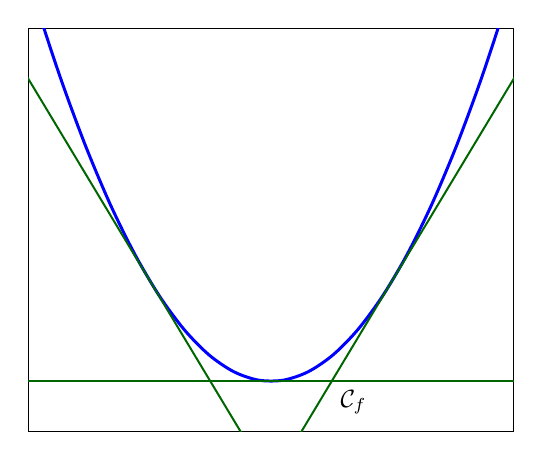
\begin{tikzpicture}[scale=0.9]
                    \begin{axis}[
                        xmin=-2, xmax=2,
                        ymin=-2, ymax=2,
                        xtick=\empty,
                        ytick=\empty
                    ]
                        \addplot[blue, very thick, samples=50, smooth]{x^2-1.5};
                        \addplot[black!60!green, thick]{-2*\x-2.5};
                        \addplot[black!60!green, thick]{-1.5};
                        \addplot[black!60!green, thick]{2*\x-2.5};
                        \node[anchor=north west] at (0.5,-1.5) {$\mathcal{C}_f$};

                    \end{axis}
                \end{tikzpicture}
                \hspace{1cm}
                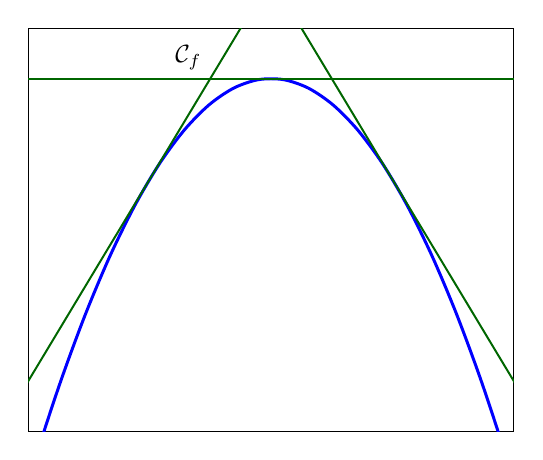
\begin{tikzpicture}[scale=0.9]
                    \begin{axis}[
                        xmin=-2, xmax=2,
                        ymin=-2, ymax=2,
                        xtick=\empty,
                        ytick=\empty
                    ]
                        \addplot[blue, very thick, samples=50, smooth]{-x^2+1.5};
                        \addplot[black!60!green, thick]{2*\x+2.5};
                        \addplot[black!60!green, thick]{-2*\x+2.5};
                        \addplot[black!60!green, thick]{1.5};
                        \node[anchor=south east] at (-0.5,1.5) {$\mathcal{C}_f$};
                    \end{axis}
                \end{tikzpicture}
                \parbox{\linewidth}{\captionof{figure}{\centering Illustration de la Propriété}}
            \end{center}
        \end{Spartie}
        \begin{Spartie}{Définition} 
            $A$ est un point d'inflexion de $\mathcal{C}$ si au point $A$, la courbe traverse sa tangente.

            \begin{center}
                \begin{tikzpicture}
                    \begin{axis}[
                        xmin=-3.25, xmax=3.25,
                        ymin=-4.25, ymax=4.25
                    ]
                        \addplot[blue, very thick, samples=50, smooth]{0.5*\x^3-1.5*\x};
                        \addplot[black!60!green, thick]{-1.5*\x};
                        \node[dot] at (0,0) {};
                        \node[anchor=south west] at (0,0) {$A$};
                    \end{axis}
                \end{tikzpicture}
                \parbox{\linewidth}{\captionof{figure}{\centering Exemple d'un Point d'Inflexion}}
            \end{center}
        \end{Spartie}
        \begin{Spartie}{Remarque} 
            Lorsque $f$ change de convexité, sa courbe $\mathcal{C}$ admet un point d'inflexion.
        \end{Spartie}
    \end{Gpartie}
    \pagebreak
    \begin{Gpartie}{Lien avec la Dérivée} 
        \begin{Spartie}{Définition} 
            Soit $f$ une fonction dérivable sur $I$ dont la fonction dérivée $f'$ est dérivable sur $I$. La dérivée de $f'$ se nomme la dérivée seconde de $f$ et se note $f''$.
        \end{Spartie}
        \begin{Spartie}{Propriété} 
            Soit $f$ une fonction dérivable deux fois sur un intervalle $I$.

            $f$ est convexe sur $I$ si et seulement si :
            \begin{itemize}
                \item $f'$ est croissante sur $I$
                \item $f''$ est positive sur $I$
                \item La courbe représentative est située au dessus de ses tangentes sur $I$
            \end{itemize}
        \end{Spartie}
        \begin{Spartie}{Propriété} 
            $f$ est concave sur $I$ si et seulement si :
            \begin{itemize}
                \item $f'$ est décroissante sur $I$
                \item $f''$ est négative sur $I$
                \item La courbe représentative est située en dessous de ses tangentes sur $I$
            \end{itemize}
        \end{Spartie}
        \begin{Spartie}{Propriété} 
            Si $\mathcal{C}$ est la courbe représentative de $f$ dans un repère, $\mathcal{C}$ admet un point d'inflexion au point d'abscisse $a$ si et seulement si $f''$ s'annule et change de signe en $a$.

            \begin{center}
                \begin{tikzpicture}
                    \begin{axis}[
                        xmin=-5.25, xmax=5.25,
                        ymin=-4.25, ymax=4.25,
                        legend pos=south east
                    ]
                        \addplot[blue, very thick, samples=50, smooth]{0.5*\x^3-1.5*\x};
                        \addplot[red, thick, samples=50, smooth]{1.5*\x^2-1.5};
                        \addplot[orange, thick, samples=50, smooth]{3*\x};
                        \addlegendentry{$f(x)$}
                        \addlegendentry{$f'(x)$}
                        \addlegendentry{$f''(x)$}
                        \node[dot] at (0,0) {};
                        \node[anchor=south west] at (0,0) {$A$};
                    \end{axis}
                \end{tikzpicture}
                \parbox{\linewidth}{\captionof{figure}{\centering Illustration de l'Évolution de la Convexité en Fonction de la Dérivée Seconde}}
            \end{center}
        \end{Spartie}
    \end{Gpartie}

    \chapter{Opérations sur les Variables Aléatoires}

    \begin{Gpartie}{Rappels} 
        Soit $\Omega$ l'univers d'une experience aléatoire.

        Une variable aléatoire $X$ est une fonction qui à tout élément de $\Omega$ associe un nombre~réel.
        \begin{Spartie}{Exemple} 
            On tire deux fois une pièce : $\Omega=\big\{~PP~,~PF~,~FP~,~FF~\big\}$.

            Soit $X$ la variable aléatoire définie sur $\Omega$ qui donne le nombre de \og pile \fg{} obtenus.

            Soit $G$ la variable aléatoire égale au gain suivant :
            \begin{itemize}
                \item Deux faces identiques ( PP et FF ) font gagner $\pounds~2$.
                \item Deux faces différentes ( PF et FP ) font perdre $\pounds~2$.
            \end{itemize}

            Les lois de probabilités des variables aléatoires $X$ et $G$ sont :

            \begin{center}\begin{tabular}{ | p{0.12\linewidth}||*{3}{>{\centering\arraybackslash}m{0.05\linewidth} | }} \hline
                $x_i$     & $0$             & $1$             & $2$             \\ \hline
                $P(X=x_i)$& $\frac{1}{4}$   & $\frac{1}{2}$   & $\frac{1}{4}$   \\ \hline
            \end{tabular}\hspace{4ex}\begin{tabular}{ | p{0.12\linewidth}||*{2}{>{\centering\arraybackslash}m{0.05\linewidth} | }} \hline
                $g_i$       & $-2$          & $2$           \\ \hline
                $P(G=g_i)$  & $\frac{1}{2}$ & $\frac{1}{2}$ \\ \hline
            \end{tabular}\end{center}
            \parbox{\linewidth}{\captionof{figure}{\centering Lois de Probabilité de X et G}}
        \end{Spartie}
        \begin{Spartie}{Définition} 
            L'espérance de la variable aléatoire $X$ est le réel : \[E(X)=\sum_{i=1}^nx_iP\left(X=x_i\right)\]
            L'espérance est une moyenne, les probabilités jouent le role de fréquences.

            Dans notre exemple, $E(X)=1$ et $E(G)=0$.
        \end{Spartie}
        \begin{Spartie}{Définition} 
            La variance de la variable aléatoire $X$ est le réel : \[V(X)=\sum_{i=1}^n\left(x_i-E(X)\right)^2P(X=x_i)\]
            C'est la moyenne des écarts au carré.
        \end{Spartie}
        \begin{Spartie}{Définition} 
            L'écart-type de la variable aléatoire $X$ est le réel : \[\sigma=\sqrt{V(X)}\]
        \end{Spartie}
        \begin{Spartie}{Théorème} 
            \[V(X)=\sum_{i=1}^nx_i^2P(X=x_i)-\left(E(X)\right)^2=E\left(X^2\right)-\left(E(X)\right)^2\]
            La variance est aussi la moyenne des valeurs au carré moins la moyenne au carré.
            \begin{SSpartie}{Démonstration} 
                $\begin{aligned}[t]
                    V(X)&=\sum_{i=1}^n\left(x_i-E(X)^2\right)p_i\qquad\left(P(X=x_i)=p_i\right) \\
                    &=\sum_{i=1}^n\left(x_i^2-2x_iE(X)+\left(E(X)\right)^2\right)p_i \\
                    &=\sum_{i=1}^n\left(x_i^2p_i\right)-2E(X)\sum_{i=1}^n x_i p_i+\left(E(X)\right)^2\sum_{i=1}^np_i \\
                    &=E\left(X^2\right)-2\left(E(X)\times E(X)\right)+\left(E(X)\right)^2\times 1 \\
                    &=E\left(X^2\right)-\left(E(X)\right)^2\quad\square
                \end{aligned}$
            \end{SSpartie}
        \end{Spartie}
    \end{Gpartie}
    \begin{Gpartie}{Opérations sur les Variables Aléatoires} 
        \begin{Spartie}{Changement Affine} 
            \begin{SSpartie}{Théorème} 
                Si $X$ est une variable aléatoire et $a$ et $b$ sont deux réels : \[(1)\quad E(aX+b)=aE(X)+b\] \[(2)\quad V(aX+b)=a^2V(X)\]
                \begin{SSSpartie}{Démonstrations}
                    On note $p_i$ la probabilité $P(X=x_i)$ pour alléger les notations.
                    \begin{enumerate}[(1),leftmargin=4ex]
                        \item $\begin{aligned}[t]
                            E(aX+b)&=\sum_{i=1}^n\left(a x_i+b\right)p_i \\
                            &=a\sum_{i=1}^n x_i p_i+b\sum_{i=1}^np_i \\
                            &=aE(X)+b\quad\square
                        \end{aligned}$
                        \item $\begin{aligned}[t]
                            V(aX+b)&=E\left((aX+b)^2\right)-\left(E(aX+b)\right)^2 \\
                            &=E\left(a^2X^2+2aXb+b^2\right)-\left(E(aX+b)\right)^2 \\
                            &=a^2E\left(X^2\right)+2abE(X)+b^2-a^2\left(E(X)\right)^2-2abE(X)-b^2 \\
                            &=a^2\left(E\left(X^2\right)-\left(E(X)\right)^2\right) \\
                            &=a^2V(X)\quad\square
                        \end{aligned}$
                    \end{enumerate}
                \end{SSSpartie}
            \end{SSpartie}
            \begin{SSpartie}{Théorème} 
                Si $X$ est une variable aléatoire et $a$ et $b$ sont deux réels : \[\sigma(aX+b)=\lvert a\rvert \sigma(X)\]
                \begin{SSSpartie}{Démonstration} 
                    $\begin{aligned}[t]
                        \sigma(aX+b)&=\sqrt{V(aX+b)} \\
                        &=\sqrt{a^2V(X)} \\ 
                        &=\lvert a\rvert\sigma(X)\quad\square
                    \end{aligned}$
                \end{SSSpartie}
            \end{SSpartie}
            \begin{SSpartie}{Exemple} 
                Dans le jeu précédent (deux tirages de pièce), si $X'$ est la variable aléatoire qui donne le triple de nombre de \og pile \fg , $X'=3X$ et donc $E\left(X'\right)=3E(X)=3$.
            \end{SSpartie}
        \end{Spartie}
        \begin{Spartie}{Somme de Variables Aléatoires} 
            Dans cette sous-partie, $X$ et $Y$ sont deux variables aléatoires prenant respectivement les valeurs $\big\{~a_1~,~a_2~,~\dotsc~,~a_n~\big\}$ et $\big\{~b_1~,~b_2~,~\dotsc~,~b_m~\big\}$, où $n$ et $m$ sont des entiers naturels non nuls.
            \begin{SSpartie}{Définition} 
                La variable aléatoire $X+Y$ prend tous les valeurs $a_i+b_j$ possibles (où $1\leq i\leq n$ et $q\leq j\leq m$).

                Pour toute valeur de $w$, $P(X+Y=w)=\sum_{a_i+b_j=w}P\left(\{X=a_i\}\cap\{Y=b_j\}\right)$ c'est-à-dire la somme des probabilités $P\left(\{X=a_i\}\cap\{Y=b_j\}\right)$ telles que $a_i+b_j=w$ (toutes les sommes égales à $w$).
            \end{SSpartie}
            \begin{SSpartie}{Théorème (admis)} 
                \[E(X+Y)=E(X)+E(Y)\]
            \end{SSpartie}
            \begin{SSpartie}{Rappel} 
                $A$ et $B$ sont deux événements indépendants si et seulement si $P\left(A\cap B\right)=P(A)\times P(B)$.
            \end{SSpartie}
            \begin{SSpartie}{Définition} 
                Deux variables aléatoires sont indépendantes si elles donnent des résultats de deux expériences aléatoires indépendantes.
            \end{SSpartie}
            \begin{SSpartie}{Propriété} 
                Si $X$ et $Y$ indépendantes : \[P\left(\{X=a_i\}\cap\{Y=b_j\}\right)=P(X=a_i)\times P(Y=b_j)\]
            \end{SSpartie}
            \begin{SSpartie}{Théorème (admis)} 
                Si $X$ et $Y$ sont deux variables aléatoires indépendantes définies sur un même~univers : \[V(X+Y)=V(X)+V(Y)\]
            \end{SSpartie}
        \end{Spartie}
    \end{Gpartie}
    \begin{Gpartie}{Applications} 
        \begin{Spartie}{Loi Binomiale} 
            \begin{SSpartie}{Propriété} 
                Si $X$ est une variable aléatoire qui suit la loi binomiale $\mathcal{B}\left(n~;p\right)$ : \[E(X)=np\qquad V(X)=np\left(1-p\right)\qquad\sigma(X)=\sqrt{np\left(1-p\right)}\]
                \begin{SSSpartie}{Démonstration} 
                    $X$ est la somme de $n$ variables aléatoires indépendantes $X_1~,~X_2~,\dotsc,~X_n~$, suivant la loi de \textsc{Bernoulli}.

                    Pour tout $i$, $1\leq i\leq n,~E\left(X_i\right)=p$ et $V\left(X_i\right)=p\left(1-p\right)$.

                    Ainsi, $E(X)=E\left(X_1\right)+E\left(X_2\right)+\dotsb+E\left(X_n\right)=np$ et idem pour $V(X)$. \\
                    Enfin, $\sigma(X)=\sqrt{V(X)}$
                \end{SSSpartie}
            \end{SSpartie}
        \end{Spartie}
        \begin{Spartie}{Somme et Moyenne d'un Échantillon (généralisation)} 
            \begin{SSpartie}{Définition} 
                Un échantillon de taille $n$ d'une loi de probabilité est une liste $\big\{~X_1~,~X_2~,~\dotsc~,~X_n~\big\}$ de $n$ variables aléatoires identiques et indépendantes qui suivent toutes cette loi.
            \end{SSpartie}
            \begin{SSpartie}{Propriété} 
                Si on note $X$ une variable aléatoire suivant la loi de probabilité de cet échantillon, la variable aléatoire \og somme \fg{} de cet échantillon $S_n=X_1+X_2+\dotsb+X_n$ vérifie : \[(1)~E\left(S_n\right)=nE(X)\qquad(2)~V\left(S_n\right)=nV(X)\qquad(3)~\sigma\left(S_n\right)=\sqrt{n}\sigma(X)\]
                \begin{SSSpartie}{Démonstration} 
                    \begin{enumerate}[(1)]
                        \item $\begin{aligned}[t]
                            E\left(S_n\right)&=E\left(X_1+X_2+\dotsb+X_n\right) \\
                            &=E(X_1)+E(X_2)+\dotsb+E(X_n) \\
                            &=nE(X)\quad\text{Car les variables sont identiques}
                        \end{aligned}$
                        \item $\begin{aligned}[t]
                            V\left(S_n\right)&=V(X_1+X_2+\dotsb+X_n) \\
                            &=V(X_1)+V(X_2)+\dotsb+V(X_n) \\
                            &=nV(X)
                        \end{aligned}$
                        \item $\begin{aligned}[t]
                            \sigma(S_n)&=\sqrt{V(S_n)} \\
                            &=\sqrt{nV(X)} \\
                            &=\sqrt{n}\sigma(X)
                        \end{aligned}$
                    \end{enumerate}
                \end{SSSpartie}
            \end{SSpartie}
            \begin{SSpartie}{Propriété} 
                Si $X$ est une variable aléatoire suivant la loi de probabilité de cet échantillon, la variable aléatoire \og moyenne \fg{} de cet échantillon $M_n=\frac{X_1+X_2+\dotsb+X_n}{n}=\frac{S_n}{n}$~vérifie~: \[(1)~E\left(M_n\right)=E(X)\qquad(2)~V(M_n)=\frac{V(X)}{n}\qquad(3)~\sigma(M_n)=\frac{\sigma(X)}{\sqrt{n}}\]
                \begin{SSSpartie}{Démonstration} 
                    \begin{enumerate}[(1)]
                        \item $\begin{aligned}[t]
                            E(M_n)&=E\left(\frac{S_n}{n}\right) \\
                            &=nE\left(\frac{X}{n}\right) \\
                            &=\frac{1}{n}\times nE(X)\qquad\text{changement affine de $\tfrac{1}{n}$}\\
                            &=E(X)
                        \end{aligned}$
                        \item $\begin{aligned}[t]
                            V(M_n)&=V\left(\frac{S_n}{n}\right) \\
                            &=nV\left(\frac{X}{n}\right) \\
                            &=\frac{1}{n^2}\times nV(X) \\
                            &=\frac{V(X)}{n}
                        \end{aligned}$
                        \item $\begin{aligned}[t]
                            \sigma(M_n)&=\sqrt{V(M_n)} \\
                            &=\frac{\sigma(X)}{\sqrt{n}}
                        \end{aligned}$
                    \end{enumerate}
                \end{SSSpartie}
            \end{SSpartie}
        \end{Spartie}
    \end{Gpartie}








    \chapter{Calcul Intégral}

    \begin{Gpartie}{Notion d'Intégrale} 
        \begin{Spartie}{Aire sous la Courbe et Intégrale} 
            \begin{SSpartie}{Défintion} 
                Soit $f$ une fonction \emph{continue et positive} sur un intervalle $\big[a~;b\big]~\left(a\leq b\right)$ et $\mathcal{C}$ sa courbe représentative dans un repère orthogonal.

                L'aire délimitée par $\mathcal{C}$, l'axe des abscisses et les droites d'équation $x=a$ et $x=b$ est l'intégrale de $f$ sur $\big[a~;b\big]$, et se note : \[\int_a^b f(t)\dt\]
            \end{SSpartie}
            \begin{SSpartie}{Remarques} 
                $\int_a^b f(t)\dt$ se lit \og intégrale de $a$ à $b$ de $f$ de $t~\dt$ \fg{} \\ ou \og somme de $a$ à $b$ de $f$ de $t~\dt$ \fg{}.

                $\int_a^b f(t)\dt$ se note indifféremment $\int_a^b f(x)\dx$

                $\int_a^b f(t)\dt$ se mesure en unité d'aire ($u.a.$). Où $1~u.a.$ est l'aire du rectangle de base (1 sur 1).
            \end{SSpartie}
            \begin{SSpartie}{Remarque} 
                Dans le cas d'une fonction continue de signe quelconque, $\int_a^b f(t)\dt$ est une aire algébrique entre la courbe, l'axe des abscisses et les droites d'équation $x=a$ et $x=b$.

                Par convention, on compte positivement les aires lorsque $\mathcal{C}$ est au dessus de l'axe des abscisses et négativement lorsqu'elle est en dessous.
            \end{SSpartie}
        \end{Spartie}
        \begin{Spartie}{Dérivabilité de la Fonction Aire} 
            \begin{SSpartie}{Théorème} 
                Soit $f$ une fonction continue et positive sur $\big[a~;b\big]~\left(a\leq b\right)$

                Alors, la fonction $\Phi:x\mapsto\int_a^xf(t)\dt$ est dérivable sur $\big[a~;b\big]$ et : \[\Phi'=f\qquad\text{($\Phi$ est une primitive de $f$)}\]
                \begin{SSSpartie}{Démonstration \big($f$ croissante\big)} 
                    Soit $x_0\in\big[a~;b\big]$ et $h\neq 0$ tel que $x_0+h\in\big[a~;b\big]$. Notons $\mathcal{C}$ la courbe représentative de $f$.

                    \begin{center}
                        \begin{tikzpicture}[scale=0.8]
                            \begin{axis}[
                                xmin=-0.25, xmax=4.25,
                                ymin=-0.3, ymax=3.75,
                                xtick=\empty,
                                ytick=\empty,
                                domain=0.5:3.75
                            ]
                                \addplot[blue, very thick]{e^(0.3*\x)};
                                \draw[dashed, thick] (0.5,0) node[label={[label distance=-6pt]below:$a$}] {} -- (0.5,1.16) node[dot] {};
                                \draw[dashed, thick] (3.75,0) node[label={[label distance=-7.5pt]below:$b$}] {} -- (3.75,3.08) node[dot] {};
                                % \draw[pattern=north west lines] (1.5,1.57) -- (1.5,0) -- (2.5,0) -- (2.5,1.57) -- cycle;
                                \draw[black!60!green, pattern=north west lines] (1.5,1.57) rectangle (2.5,0);
                                \draw[red,pattern=north west lines] (1.5,1.57) rectangle (2.5,2.12);
                                \node[anchor=north,inner sep=2pt] at (1.5,0) {$x_0$};
                                \node[anchor=north,inner sep=2pt] at (2.5,0) {$x_{0+h}$};

                            \end{axis}
                        \end{tikzpicture}
                        \parbox{\linewidth}{\captionof{figure}{\centering Encadrement de la Fonction $\Phi$}}
                    \end{center}

                    Étudions $\lim\limits_{h\to0}\dfrac{\Phi\left(x_0+h\right)-\Phi\left(x_0\right)}{h}$

                    $\Phi\left(x_0+h\right)-\Phi(x_0)$ est l'aire sous la courbe entre $x_0$ et $x_0+h$.

                    On encadre cette aire par les aires des deux rectangles de largeur $\lvert h\rvert$ et de hauteur $f(x_0)$ (en vert) et $f(x_0+h)$ (en rouge)

                    \begin{itemize}
                        \item Si $h>0$, et comme $f$ est croissante :
                        
                        $\begin{aligned}[t]
                            &\quad h\times f(x_0)\leq\Phi\left(x_0+h\right)-\Phi(x_0)\leq h\times f(x_0+h) \\
                            \iff&\quad f(x_0)\leq \frac{\Phi\left(x_0+h\right)-\Phi(x_0)}{h}\leq f(x_0+h) 
                        \end{aligned}$

                        \item Si $h<0$ alors la largeur est $-h$ :
                        
                        $\begin{aligned}[t]
                            &\quad -h\times f(x_0+h)\geq\Phi(x_0)-\Phi(x_0+h)\geq -h\times f(x_0) \\
                            \iff&\quad f(x_0+h)\leq\frac{\Phi\left(x_0+h\right)-\Phi(x_0)}{h}\leq f(x_0)
                        \end{aligned}$
                    \end{itemize}
                    Or $f$ est continue, donc $\lim\limits_{h\to0}f(x_0+h)=f(x_0)$

                    Donc, d'après le théorème des gendarmes : \[\lim\limits_{h\to0}\frac{\Phi\left(x_0+h\right)-\Phi(x_0)}{h}=f(x_0)\quad\square\]

                    Ainsi, $\Phi$ est dérivable en $x_0$ et $\Phi'(x_0)=f(x_0)$.

                    Ce résultat est vrai pour tout $x_0\in I$, donc $\Phi$ est dérivable sur $I$ et $\Phi'=f$.
                \end{SSSpartie}
            \end{SSpartie}
            \begin{SSpartie}{Rappel Théorème} 
                Soit $f$ une fonction continue sur $I$ et $\Phi$ une primitive de $f$ sur $I$.

                Alors, $f$ admet une infinité de primitives sur $I$ et toute primitive $F$ de $f$ est définie par $F(x)=\Phi(x)+k,~k\in\mathbb{R}$.
            \end{SSpartie}
            \begin{SSpartie}{Conséquence} 
                Soit $f$ une fonction continue et positive sur $\big[a~;b\big]$.

                Le premier théorème prouve l'existence d'une primitive $\Phi$ de $f$ sur $\big[a~;b\big]$, définie par $\Phi(x)=\int_a^xf(t)\dt$.

                Ainsi, $\int_a^b f(t)\dt=\Phi(b)$

                Et d'après le deuxième théorème (lien entre deux primitives), quelle que soit $F$,~la primitive de $f$, il existe un réel $k$ tel que $F=\Phi+k$. \\ Donc, $F(a)=\Phi(a)+k=k$ car $\Phi(a)=\int_a^af(t)\dt=0$.

                Ainsi, $\Phi(b)=F(b)-k=F(b)-F(a)$

                Or $\Phi(b)=\int_a^b f(t)\dt$
                
                Donc, quelle que soit la primitive $F$ de $f$ : \[\int_a^b f(t)\dt=F(b)-F(a)\]
            \end{SSpartie}
            \begin{SSpartie}{Remarque} 
                On note : \[\int_a^b f(t)\dt=\big[F(t)\big]_a^b=F(b)-F(a)\]
            \end{SSpartie}
            \begin{SSpartie}{Exemples} 
                \begin{itemize}
                    \item $\displaystyle \int_0^1\me^x\dx=\big[\me^x\big]_0^1=\me^1-\me^0=\me-1$
                    \item $\displaystyle \int_0^2t^2\dt=\Bigg[\frac{t^3}{3}\Bigg]_0^2=\frac{2^3}{3}-\frac{0^3}{3}=\frac{8}{3}$
                \end{itemize}
            \end{SSpartie}
        \end{Spartie}
    \end{Gpartie}
    \begin{Gpartie}{Intégrale d'une Fonction Continue} 
        \begin{Spartie}{Extension de la Notion d'Intégrale} 
            On a défini l'intégrale d'une fonction $f$ continue et positive sur un intervalle $\big[a~;b\big]~\left(a\leq b\right)$, et on a vu que si $F$ est une primitive de $f$ sur $\big[a~;b\big]$ : \[\int_a^b f(t)\dt=F(b)-F(a)\]

            On admet que cette formule peut être étendue au cas d'une fonction continue de signe quelconque, quelles que soient les bornes $a$ et $b$ de l'intégrale.

            \begin{SSpartie}{Définition} 
                Soit $f$ une fonction continue sur un intervalle $I$ et soit $F$ une primitive de $f$ sur $I$. Si $a$ et $b$ sont deux réels quelconques de $I$, l'intégrale de $f$ entre $a$ et $b$ s'écrit : \[\int_a^b f(t)\dt=\big[F(t)\big]_a^b=F(b)-F(a)\]
            \end{SSpartie}
            \begin{SSpartie}{Exemples} 
                \begin{itemize}
                    \item   
                    $\begin{aligned}[t]
                        \int_{-4}^{-2}\left(\frac{1}{t^2}-3\right)\dt=\Bigg[\frac{-1}{t}-3t\Bigg]_{-4}^{-2}&=\frac{-1}{(-2)}-3\times(-2)-\left(\frac{-1}{(-4)}-3\times(-4)\right)  \\
                        &=\frac{1}{2}+6-\frac{1}{4}-12 \\
                        &=\frac{-23}{4}
                    \end{aligned}$

                    \item 
                    $\begin{aligned}[t]
                        \int_\frac{1}{2}^1\left(\frac{1}{t}-t^2\right)\dt=\Bigg[\ln\,(t)-\frac{t^3}{3}\Bigg]_\frac{1}{2}^1&=\ln\,(1)-\frac{1}{3}-\left(\ln\,\left(\tfrac{1}{2}\right)-\frac{\left(\frac{1}{2}\right)^3}{3}\right) \\
                        &=\frac{-1}{3}+\ln\,(2)+\frac{1}{24} \\
                        &=\frac{7}{24}+\ln\,(2)
                    \end{aligned}$
                    \item 
                    $\begin{aligned}[t]
                        \int_{-2}^1t\dt=\Bigg[\frac{t^2}{2}\Bigg]_{-2}^1&=\frac{1^2}{2}-\frac{(-2)^2}{2} \\
                        &=\frac{3}{2}
                    \end{aligned}$
                \end{itemize}
            \end{SSpartie}
            \begin{SSpartie}{Conséquences} 
                \begin{itemize}
                    \item $\displaystyle\int_a^af(t)\dt=0\quad\big(=F(a)-F(a)\big)$
                    \item $\displaystyle\int_b^af(t)\dt=F(a)-F(b)=-\int_a^b f(t)\dt$
                \end{itemize}
            \end{SSpartie}
        \end{Spartie}
        \begin{Spartie}{Linéarité de l'Intégrale} 
            \begin{SSpartie}{Théorème} 
                Soient $f$ et $g$ deux fonctions continues sur $I$ et soit $\lambda$ un réel. Pour tous réels $a$ et $b$ de $I$ : \[\int_a^b\left(f+g\right)(t)\dt=\int_a^b f(t)\dt+\int_a^bg(t)\dt\] \[\int_a^b\lambda f(t)\dt=\lambda\int_a^b f(t)\dt\]
                \begin{SSSpartie}{Démonstration} 
                    Soient $F$ et $G$ des primitives de $f$ et $g$. Alors $F+G$ et $\lambda F$ sont des primitives de $f+g$ et $\lambda f$ respectivement.
                    \begin{itemize}
                        \item 
                        $\begin{aligned}[t]
                            \int_a^b\left(f+g\right)(t)\dt&=\left(F+G\right)(t)-\left(F+G\right)(t) \\
                            &=F(b)+G(b)-F(a)-G(a) \\
                            &=F(b)-F(a)+G(b)-G(a) \\
                            &=\int_a^b f(t)\dt+\int_a^b g(t)\dt
                        \end{aligned}$

                        \item $\begin{aligned}[t]
                            \int_a^b\lambda f(t)\dt&=\lambda F(b)-\lambda F(a) \\
                            &=\lambda\left(F(b)-F(a)\right) \\
                            &=\lambda\int_a^b f(t)\dt
                        \end{aligned}$
                    \end{itemize}
                \end{SSSpartie}
            \end{SSpartie}
        \end{Spartie}
        \begin{Spartie}{Relation de Chasles} 
            \begin{SSpartie}{Théorème} 
                Soit $f$ une fonction continue sur un intervalle $I$. Quels que soient les réels $a$, $b$ et $c$ appartenant à $I$ : \[\int_a^c f(t)\dt=\int_a^b f(t)\dt+\int_b^cf(t)\dt\]
                \begin{SSSpartie}{Démonstration} 
                    Soit $F$ une primitive de $f$.

                    $\begin{aligned}[t]
                        \int_a^c f(t)\dt&=F(c)-F(a) \\
                        &=F(c)-F(b)+F(b)-F(a) \\
                        &=\int_a^b f(t)\dt+\int_b^c f(t)\dt
                    \end{aligned}$
                \end{SSSpartie}
            \end{SSpartie}
            \begin{SSpartie}{Remarque} 
                Dans le cas où $f$ est positive et $a\leq b\leq c$, la relation de Chasles traduit l'additivité des aires de deux domaines adjacents.
            \end{SSpartie}
            \begin{SSpartie}{Exemple} 
                Intégrale d'une fonction définie par morceaux : \[\int_{-2}^5f(x)\dx\quad\text{où}\quad f:x\mapsto\lvert x\rvert-2\qquad\lvert x\rvert\begin{cases}x\geq0:x\\x<0:-x\end{cases}\]

                $\begin{aligned}[t]
                    \int_{-2}^5f(x)\dx &= \int_{-2}^0f(x)\dx+\int_0^5f(x)\dx \\
                    &= \Bigg[\frac{-x^2}{2}-2x\Bigg]_{-2}^0+\Bigg[\frac{x^2}{2}-2x\Bigg]_0^5 \\
                    &= 0-2+\frac{5}{2}-0=\frac{1}{2} 
                \end{aligned}$
            \end{SSpartie}
        \end{Spartie}
        \begin{Spartie}{Positivité et Ordre} 
            \begin{SSpartie}{Théorème} 
                Soit $f$ une fonction continue sur $I$, et $a$ et $b$ deux réels de $I$ tels que $a\leq b$

                Si $\forall t\in I,~f(t)\geq0$ : \[\int_a^b f(x)\dt\geq0\]
                \begin{SSSpartie}{Démonstration} 
                    Dans le cas d'une fonction continue et positive sur $\big[a~;b\big],~\int_a^b f(t)\dt$ est l'aire sous la courbe représentative de $f$ entre $a$ et $b$, elle est positive.
                \end{SSSpartie}
            \end{SSpartie}
            \begin{SSpartie}{Théorème} 
                Soient $f$ et $g$ deux fonctions continues sur un intervalle $I$ et $a$ et $b$ deux réels tels que $a\leq b$

                Si $\forall t\in I,~f(t)\leq g(t)$ : \[\int_a^b f(t)\dt\leq\int_a^bg(t)\dt\]
                \begin{SSSpartie}{Démonstration} 
                    $g-f$ est positive sur $I$ donc : 

                    $\begin{aligned}[t]
                        &\quad\int_a^b\left(g-f\right)(t)\dt\geq 0 \\
                        \iff&\quad\int_a^b g(t)\dt-\int_a^b f(t)\dt\geq 0 \\
                        \iff&\quad\int_a^b f(t)\dt\leq\int_a^b g(t)\dt
                    \end{aligned}$
                \end{SSSpartie}
            \end{SSpartie}
        \end{Spartie}
    \end{Gpartie}
    \pagebreak
    \begin{Gpartie}{Valeur Moyenne d'une Fonction Continue} 
        \begin{Spartie}{Valeur Moyenne} 
            \begin{SSpartie}{Définition} 
                Soit $f$ une fonction continue sur un intervalle $\big[a~;b\big]$, avec $a<b$, la valeur moyenne de la fonction $f$ sur $\big[a~;b\big]$ est le nombre $\mu$ défini par : \[\mu=\frac{1}{b-a}\int_a^b f(t)\dt\]
            \end{SSpartie}
            \begin{SSpartie}{Remarque} 
                Interprétation dans le cas d'une fonction positive : \[\int_a^b f(t)\dt=\mu(b-a)\]
                \begin{center}
                    \begin{tikzpicture}
                        \begin{axis}[
                            xmin=-0.5, xmax=5,
                            ymin=-0.5, ymax=5,
                            xtick=\empty,
                            ytick=\empty,
                            domain=1:4
                        ]
                            \addplot[name path=a,blue, very thick]{0.7*(\x-2.5)^3-\x+5.5};
                            \draw (0,3.06) node[anchor=east] {$\mu$} -- (5,3.06);
                            \node[anchor=north] at (2.5,0) {$b-a$};

                            \path[name path=axis] (axis cs:1,0) -- (axis cs:4,0);

                            \addplot [
                                thick,
                                color=blue,
                                fill=blue, 
                                fill opacity=0.2
                            ]
                            fill between[
                                of=a and axis,
                                soft clip={domain=1:4},
                            ];

                        \end{axis}
                    \end{tikzpicture}
                    \hspace{0.5cm}
                    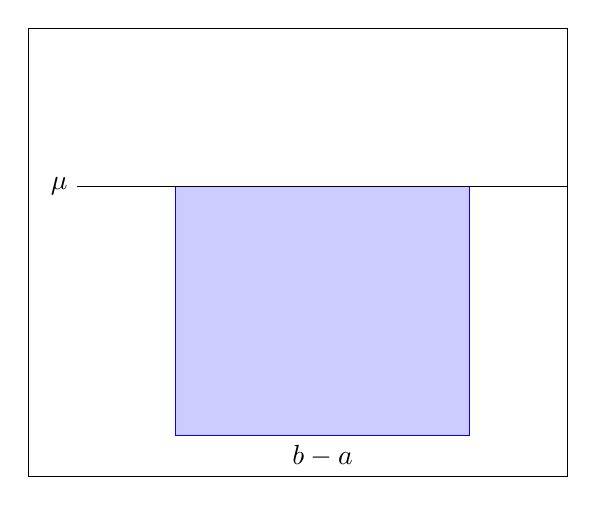
\begin{tikzpicture}
                        \begin{axis}[ 
                            xmin=-0.5, xmax=5,
                            ymin=-0.5, ymax=5,
                            xtick=\empty,
                            ytick=\empty
                        ]
                            \draw[color=blue, fill=blue, fill opacity=0.2] (1,0) rectangle (4,3.06);
                            \draw (0,3.06) node[anchor=east] {$\mu$} -- (5,3.06);
                            \node[anchor=north] at (2.5,0) {$b-a$};
                        \end{axis}
                    \end{tikzpicture}
                    \parbox{\linewidth}{\captionof{figure}{\centering Interprétation Graphique de la Valeur Moyenne pour une Fonction Positive}}
                \end{center}

                $\mu$ est la hauteur du rectangle de largeur $b-a$ dont l'aire est la même que celle du domaine situé en sous la courbe $\mathcal{C}_f$ entre $a$ et $b$.
            \end{SSpartie}
        \end{Spartie}
        \begin{Spartie}{Inégalité de la Moyenne (encadrement \og grossier \fg{} de l'intégrale)} 
            \begin{SSpartie}{Théorème} 
                Soit $f$ une fonction continue sur $\big[a~;b\big]$, $a<b$ et $m$ et $M$ deux réels tels que $\forall x\in\big[a~;b\big],~m\leq f(x)\leq M$

                On a donc : \[m(b-a)\leq\int_a^b f(t)\dt\leq M(b-a)\]
                \begin{SSSpartie}{Démonstration} 
                    $\begin{aligned}[t]
                        &\quad m\leq f(t)\leq M \\
                        \iff&\quad\big[mx\big]_a^b\leq\int_a^b f(t)\dt\leq \big[Mx\big]_a^b\quad\text{(positivité de l'intégrale)} \\
                        \iff&\quad m(b-a)\leq\int_a^b f(t)\dt \leq M(b-a)\quad\square
                    \end{aligned}$
                \end{SSSpartie}
            \end{SSpartie}
            \begin{SSpartie}{Remarques} 
                Interprétation en cas d'une fonction positive : L'aire de la courbe $\mathcal{C}_f$ est comprise entre les aires des rectangles de longueur $b-a$ et de hauteurs respectives $m$ et $M$.
                
                Encadrement de la valeur moyenne :

                $\begin{aligned}[t]
                    &\quad m(b-a)\leq\int_a^b f(t)\dt \leq M(b-a) \\
                    \iff&\quad m\leq\frac{\int_a^b f(t)\dt}{b-a}\leq M \\
                    \iff&\quad m\leq\mu\leq M
                \end{aligned}$
            \end{SSpartie}
        \end{Spartie}
    \end{Gpartie}
    \vfill\pagebreak
    \begin{Gpartie}{Intégration par Parties} 
        \begin{Spartie}{Propriété} 
            Soient $u$ et $v$ deux fonction dérivables telles que leurs dérivées $u'$ et $v'$ sont continues sur un intervalle $\big[a~;b\big]$. Alors : \[\int_a^b u(x)v'(x)\dx=\big[u(x)v(x)\big]_a^b-\int_a^b u'(x)v(x)\]
            \begin{SSpartie}{Démonstration} 
                Pour toute fonction $f$ dérivable dont la dérivée $f'$ est continue sur $\big[a~;b\big]$ :

                $\displaystyle \int_a^b f'(x)\dx=f(b)-f(a)=\big[f(x)\big]_a^b$\quad En effet, $f$ est un primitive de $f'$.

                Ainsi : \[\displaystyle \int_a^b (u v)'(x)\dx=\big[u(x)v(x)\big]_a^b\]

                Or : 
                \[\begin{aligned}[t]
                    \int_a^b (u v)'(x)\dx &= \int_a^b u'(x)v(x)+u(x)v'(x)\dx \\
                    &=\int_a^b u'(x)v(x)\dx + \int_a^b u(x)v'(x)\dx\quad\text{(linéarité)}
                \end{aligned}\]

                On a donc :
                \[\begin{aligned}[t]
                    &\quad\big[u(x)v(x)\big]_a^b = \int_a^b u'(x)v(x)\dx + \int_a^b u(x)v'(x)\dx \\
                    \iff&\quad\int_a^b u(x)v'(x)\dx=\big[u(x)v(x)\big]_a^b-\int_a^b u'(x)v(x)\dx\quad\square
                \end{aligned}\]
            \end{SSpartie}
        \end{Spartie}
    \end{Gpartie}





\chapter{Fonctions Trigonométriques}

    \begin{Gpartie}{Définition et Propriétés} 
        \begin{Spartie}{Rappel} 
            Soit un réel $x$ et $M$ le point correspondant sur le cercle trigonométrique dans une repère orthonormé $\left(O~;\vec{\imath}~,\vec{\jmath}\right)$.

            Le cosinus de $x$ est noté $\cos\,(x)$, où $\cos\,(x)$ est l'abscisse du point $M$. \\
            Le sinus de $x$ est noté $\sin\,(x)$, où $\sin\,(x)$ est l'ordonnée du point $M$.
            
            \begin{center}
                \begin{tikzpicture}[scale=2]
                    \draw (0,-1.25) -- (0,1.25);
                    \draw (-1.25,0) -- (1.25,0) coordinate (a) ;
                    \draw[very thick] (0,0) circle (1);
                    \draw[-stealth, red, thick] (0,0) coordinate (b) -- (0.54,0.84) coordinate (c);
                    \draw pic["$\alpha$", draw=orange, <->, angle eccentricity=1.2, angle radius=0.75cm]
                    {angle=a--b--c};
                    \draw[dashed] (0.54,0) node[label={[label distance=-5pt]below:$\sin\,(x)$}] {} -- (c);
                    \draw[dashed] (0,0.84) node[label={[label distance=-5pt]below left:$\cos\,(x)$}] {} -- (c);

                    \node[dot,label={[label distance=-2pt]above right:$M$}] at (c) {};
                \end{tikzpicture}
                \parbox{\linewidth}{\captionof{figure}{\centering Cercle Trigonométrique}}
            \end{center}
        \end{Spartie}
        \begin{Spartie}{Définitions} 
            La fonction qui à tout réel $x$ associe le nombre $\cos\,(x)$ est appelée fonction cosinus. \\
            La fonction qui à tout réel $x$ associe le nombre $\sin\,(x)$ est appelée fonction sinus.
        \end{Spartie}
        \begin{Spartie}{Propriété} 
            Quel que soit le réel $x$, $\cos\,(-x)=\cos\,(x)$, la fonction est donc \emph{paire}. \\
            Quel que soit le réel $x$, $\sin\,(-x)=-\sin\,(x)$, la fonction est donc \emph{impaire}.
        \end{Spartie}
        \begin{Spartie}{Propriété (Periodicité)} 
            Pour tout réel $x$, $\cos\,(x+2\pi)=\cos\,(x)$ et $\sin\,(x+2\pi)=\sin\,(x)$.

            Les fonctions cosinus et sinus sont donc \emph{périodiques de période} $2\pi$ ($2\pi$-périodiques).
        \end{Spartie}
        \begin{Spartie}{Remarque} 
            Ces deux propriétés permettent de réduire l'intervalle d'étude des fonctions cosinus et sinus à $\big[0~;\pi\big]$.

            Par parité, on peut déduire $\big[-\pi~;0\big]$, donc $\big[-\pi~;\pi\big]$.
            
            Par périodicité on peut déduire les résultats sur $\mathbb{R}$.
        \end{Spartie}
    \end{Gpartie}
    \begin{Gpartie}{Dérivabilité} 
        \begin{Spartie}{Étude des Fonctions Sinus et Cosinus} 
            \begin{SSpartie}{Théorème} 
                Les fonctions sinus et cosinus sont dérivables sur $\mathbb{R}$, et pour tout réel $x$~: \[\boxed{\sin'(x)=\cos\,(x)}\quad\text{et}\quad\boxed{\cos'(x)=-\sin\,(x)}\]
            \end{SSpartie}
            \begin{SSpartie}{Tableaux de Variation} 
                \begin{center}
                    \begin{tikzpicture}[scale=0.8]
                        \tkzTabInit[lgt=4, espcl=1.3]{$x$ /1 , $\cos'(x)=-\sin\,(x)$ /1 , $\cos$ /1.5}{$0$ , $\frac{\pi}{2}$ , $\pi$}
                        \tkzTabLine{ z ,  , - ,  , z }
                        \tkzTabVar{ + / $1$ , R , - / $-1$}
                        \tkzTabVal{1}{3}{0.5}{}{0}
                    \end{tikzpicture}
                    \begin{tikzpicture}[scale=0.8]
                        \tkzTabInit[lgt=4, espcl=1.3]{$x$ /1 , $\sin'(x)=\cos\,(x)$ /1 , $\sin$ /1.5}{$0$ , $\frac{\pi}{2}$ , $\pi$}
                        \tkzTabLine{ + ,  , z ,  , + }
                        \tkzTabVar{ - / $0$ , + / $1$ , - / $0$}
                    \end{tikzpicture}
                    \parbox{\linewidth}{\captionof{figure}{\centering Tableaux de Variation des Fonctions cosinus et sinus}}
                \end{center}
            \end{SSpartie}
            \begin{SSpartie}{Courbes Représentatives} 
                \begin{center}
                    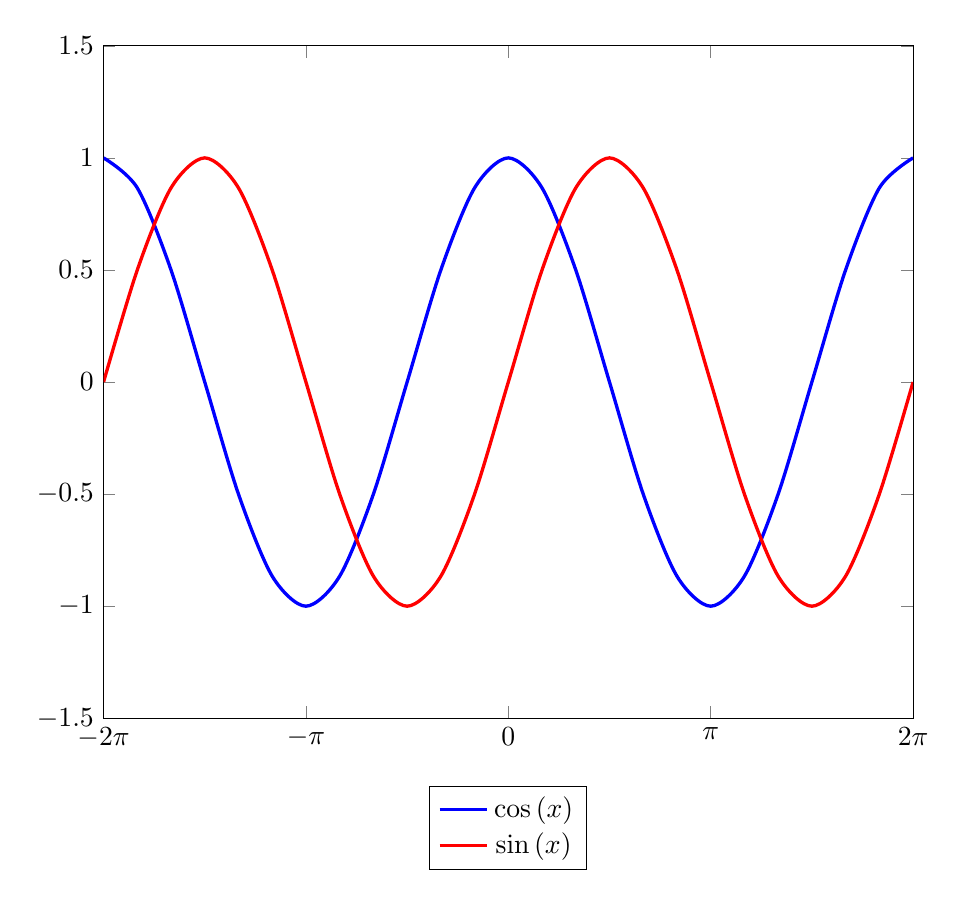
\begin{tikzpicture}
                        \begin{axis}[scale=1.5,
                            % height=0.3\linewidth, width=0.49\linewidth,
                            xmin=-2*pi, xmax=2*pi,
                            ymin=-1.5, ymax=1.5,
                            domain=-2*pi:2*pi,
                            xtick={-2*pi,-pi,0,pi,2*pi},
                            xticklabels={$-2\pi$,$-\pi$,$0$,$\pi$,$2\pi$},
                            legend style={at={(0.5,-0.1)},anchor=north}
                        ]
                            \addplot[smooth, blue, very thick]{cos(deg(\x))};
                            \addlegendentry{$\cos\,(x)$};
                            \addplot[smooth, red, very thick]{sin(deg(\x))};
                            \addlegendentry{$\sin\,(x)$};
                        \end{axis}
                    \end{tikzpicture}
                    \parbox{\linewidth}{\captionof{figure}{\centering Représentation Graphique des Fonctions cosinus et sinus}}
                \end{center}
            \end{SSpartie}
        \end{Spartie}
        \pagebreak
        \begin{Spartie}{Complément} 
            \begin{SSpartie}{Théorème} 
                \[\lim\limits_{x\to0}\frac{\sin\,(x)}{x}=1\] \[\lim\limits_{x\to0}\frac{\cos\,(x)-1}{x}=0\]
                \begin{SSSpartie}{Démonstration} 
                    La fonction sinus est continue et dérivable en $0$ : \[\lim\limits_{h\to0}\frac{\sin\,(0+h)-\sin\,(0)}{h}=\sin'(0)=\cos\,(0)=1\quad\square\] \[\lim\limits_{h\to0}\frac{\cos\,(0+h)-\cos\,(0)}{h}=\cos'(0)=-\sin\,(0)=0\quad\square\]
                \end{SSSpartie}
            \end{SSpartie}
        \end{Spartie}
    \end{Gpartie}




    \chapter{Loi des Grands Nombres}

    \begin{Gpartie}{Inégalités Probabilitstes} 
        \begin{Spartie}{Inégalité de Markov} 
            Pour toute variable aléatoire $X$ à valeurs positives, et pour tout nombre réel $\delta$ strictement positif : \[\Pde\big(X\geq\delta\big)\leq\frac{E(X)}{\delta}\]
            \begin{SSpartie}{Démonstration} 
                $\begin{aligned}[t]
                    E(X) &= \sum_{i=1}^n x_i\Pde(X=x_i) \\
                    &= \overbrace{\sum_{x_i<\delta} x_i\Pde(X=x_i)}^{\geq0} + \sum_{x_i\geq\delta} x_i\Pde(X=x_i) \\
                    &\geq\sum_{x_i\geq\delta} x_i\Pde(X=x_i)\quad\text{on minore}\\
                    &\geq\sum_{x_i\geq\delta} \delta\Pde(X=x_i)=\delta\overbrace{\sum_{x_i\geq\delta}\Pde(X=x_i)}^{\Pde\big(X\geq\delta\big)}\quad\text{car $x_i\geq\delta$ on minore encore}
                \end{aligned}$

                $\begin{aligned}[t]
                    &\quad E(X)\geq\delta\Pde(X\geq\delta) \\
                    \iff&\quad \Pde(X\geq\delta)\leq\frac{E(X)}{\delta}
                \end{aligned}$
            \end{SSpartie}
        \end{Spartie}
        \begin{Spartie}{Inégalité de Bienaymé-Tchebychev} 
            Pour toute variable aléatoire $X$, et pour tout nombre réel $\delta$ strictement positif : \[\boxed{\Pde\big(\lvert X-E(X)\rvert\geq\delta\big)\leq\frac{V(X)}{\delta^2}}\]
            \begin{SSpartie}{Démonstration} 
                $\Pde\big(\lvert X-E(X)\rvert\geq\delta\big)=\Pde\left(\left(X-E(X)\right)^2\geq\delta^2\right)$

                D'après l'inégalité de \textsc{Markov} : \[\Pde\left(\left(X-E(X)\right)^2\geq\delta^2\right)\leq\frac{\overbrace{E\left(\left(X-E(X)\right)^2\right)}^{V(X)}}{\delta^2}\quad\square\]
            \end{SSpartie}
        \end{Spartie}
        \begin{Spartie}{Remarque} 
            Souvent, on prendre $\delta=\sigma$ ou $k\sigma$ car l'écart type $\sigma$ d'une variable aléatoire $X$ est l'unité naturelle pour étudier la dispersion de $X$ autour de sons espérance.

            L'inégalité de \textsc{Bienaymé-Tchebychev} montre notamment que des écarts de $X$ à $E(X)$ de quelques $\sigma$ deviennent improbables.
        \end{Spartie}
        \begin{Spartie}{Remarque} 
            L'Inégalité de Bienaymé-Tchebychev est loin de donner le meilleur majorant.

            Si $X$ est une variable aléatoire suivant la loi binomiale $\mathcal{B}\left(n~;p\right)$, on a $\Pde\big(\vert X-E(X)\rvert\geq 2\sigma\big)\approx 0,05$ ce qui est bien meilleur que le $0,25$ obtenu avec l'inégalité.

            En effet, si $\delta=2\sigma$ et $X\sim\mathcal{B}(~n~;~p~)$ : \[\frac{V(X)}{\delta^2}=\frac{np(1-p)}{\left(4\sqrt{np(1-p)}\right)^2}=\frac{1}{4}\]
        \end{Spartie}
    \end{Gpartie}



    \begin{Gpartie}{Loi des Grands Nombres}
        \vspace*{-2ex}
        \begin{Spartie}{Propriété} 
            Soit une variable aléatoire $X$ associée à un échantillon $\big(~X_1~,~X_2~,\dotsc,~X_n~\big)$, c'est-à-dire que $\big(~X_1~,~X_2~,\dotsc,~X_n~\big)$ est un échantillon de $n$ variables aléatoires identiques et indépendantes qui suivent toutes la loi de probabilité suivie par $X$. \ \\ On note $M_n$ la moyenne de cet échantillon. 
            
            Alors, pour tout réel $\delta>0$ : \[\Pde\big(\lvert M_n-E(X)\rvert\geq\delta\big)\leq\frac{V(X)}{n\delta^2}\quad\text{(c'est l'inégalité de concentration)}\]\[\boxed{\lim\limits_{n\to +\infty}\Pde\big(\lvert M_n-E(X)\rvert\geq\delta\big)=0}\quad\text{(c'est la loi des grands nombres)}\]

            Autrement dit, plus la taille $n$ d'un échantillon d'une variable aléatoire $X$ est grande, plus l'écart entre la moyenne de cet échantillon et l'espérance de $X$ est faible.
            \begin{SSpartie}{Démonstration} 
                \vspace*{-2ex}
                \begin{SSSpartie}{Rappels} 
                    Si $X$ et $Y$ sont deux variables aléatoires avec $Y$ telle que $Y=aX+b$ alors :
                    \begin{itemize}
                        \item $E(Y)=aE(X)+b\quad\text{et}\quad V(Y)=a^2V(X)$
                        \item $E(X+Y)=E(X)+E(Y)\quad\text{et, si $X$ et $Y$ indépendantes}\quad \mbox{V(X+Y)=V(X)+V(Y)}$
                    \end{itemize}

                    Pour un échantillon $\big\{~X_1~;X_2~;\dotsb;X_n ~\big\}$ où $X_i$ sont indépendantes, et suivent une loi $X$ :
                    \begin{itemize}
                        \item $S_n=X_1+X_2+\dotsb+X_n$\quad$E\left(S_n\right)=nE(X)$\quad$V\left(S_n\right)=nV(X)$
                        \item $M_n=\frac{S_n}{n}$\quad$E\left(M_n\right)=E(X)$\quad$V\left(M_n\right)=\frac{V(X)}{n}$
                    \end{itemize}
                \end{SSSpartie}
                Suite Démonstration :

                $\begin{aligned}[t]
                    &\quad \Pde(\rvert X-E(X)\rvert\geq\delta)\leq\frac{V(X)}{n\delta^2} \\
                    \iff&\quad\Pde(\lvert M_n-E(M_n)\rvert\geq\delta)\leq\frac{V(M_n)}{\delta}\quad\text{Inégalité de \textsc{Bienaymé-Tchébychev}} \\
                    \iff&\quad\Pde(\lvert M_n-E(X)\rvert\geq\delta)\leq\frac{V(X)}{n\delta^2}
                \end{aligned}$ \\
                On a donc, pour un $\delta$ fixe : \[0\leq\Pde(\lvert M_n-E(X)\rvert\geq\delta)\leq\frac{V(X)}{n\delta^2}\]
                Et, $\lim\limits_{n\to +\infty}\frac{V(X)}{n\delta^2}=0$, donc, d'après le théorème des Gendarmes : \[\lim\limits_{n\to +\infty}\Pde(\lvert M_n-E(X)\rvert\geq\delta)\leq\frac{V(X)}{n\delta^2}=0\]
            \end{SSpartie}
        \end{Spartie}
    \end{Gpartie}


    \let\oldfrac\frac
    \let\frac\tfrac % lazy inline style in trig functions

    \chapter{Complément sur la Trigonométrie}

    \begin{Gpartie}{Rappels}
        $\forall x\in\mathbb{R},~
        \begin{aligned}[t]&\cos\,\left(\frac{\pi}{2}-x\right)=\sin\,(x) \\
            &\sin\,\left(\frac{\pi}{2}-x\right)=\cos\,(x) \\
            &\cos^2(x)+\sin^2(x)=1 \\
            &\sin\,(x)=-\sin\,(-x) \\
            &\cos\,(x)=\cos\,(-x)
        \end{aligned}$
    \end{Gpartie}

    \begin{Gpartie}{Formules d'Addition et Duplication} 
        \begin{Spartie}{Formule d'Addition} 
            \begin{center}
                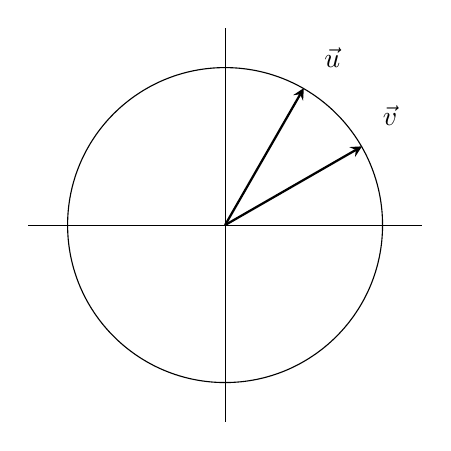
\begin{tikzpicture}[scale=2]
                    \draw (0,0) coordinate (o) circle (1);
                    \draw (-1.25,0) -- (1.25,0) coordinate (a);
                    \draw (0,-1.25) -- (0,1.25);
                    \coordinate (u) at (0.5,0.87);
                    \coordinate (v) at (0.87,0.5);
                    \draw[-stealth, thick] (0,0) -- (u) node[label=above right:$\vec{u}$] {};
                    \draw[-stealth, thick] (0,0) -- (v) node[label=above right:$\vec{v}$] {};
                    % \draw pic["$a$", draw=orange, <->, angle eccentricity=1.2, angle radius=0.75cm]{angle=a--o--u};
                \end{tikzpicture}
                \parbox{\linewidth}{\captionof{figure}{\centering Représentation de $\vec{u}$ et $\vec{v}$ dans le Cercle Trigonométrique}}
                $\lvert\lvert\vec{u}\rvert\rvert=\lvert\lvert\vec{v}\rvert\rvert=1\quad\left(\overrightarrow{OI}~;\vec{u}\right)=a\quad\left(\overrightarrow{OI}~;\vec{v}\right)=b\quad\vec{u}\begin{psmallmatrix}\cos a \\ \sin a\end{psmallmatrix}\quad\vec{v}\begin{psmallmatrix}\cos a \\ \sin a\end{psmallmatrix}$
            \end{center}

            Or, $\vec{u}\cdot\vec{v}=\cos\,(a)\cos\,(b)+\sin\,(a)\sin\,(b)$
            
            Mais, $\vec{u}\cdot\vec{v}=\lvert\lvert\vec{u}\rvert\rvert\times\lvert\lvert\vec{v}\rvert\rvert\times\cos\,(~\vec{u}~;~\vec{v}~)\quad$ avec $(~\vec{u}~;~\vec{v}~)=a-b$ ou $b-a$ 

            Ainsi : \[\cos\,(a-b)=\cos\,(a)\cos\,(b)+\sin\,(a)\sin\,(b)\]
            \begin{SSpartie}{Exemple} 
                $\begin{aligned}[t]
                    \cos\,\left(\frac{\pi}{12}\right)=\cos\,\left(\frac{\pi}{3}-\frac{\pi}{4}\right) &= \cos\,\left(\frac{\pi}{3}\right)\cos\,\left(\frac{\pi}{4}\right)+\sin\,\left(\frac{\pi}{3}\right)\sin\,\left(\frac{\pi}{4}\right) \\
                    &= \dfrac{1}{2}\times\dfrac{\sqrt{2}}{2}+\dfrac{\sqrt{3}}{2}\times\dfrac{\sqrt{2}}{2} \\
                    &= \dfrac{\sqrt{2}+\sqrt{6}}{4}
                \end{aligned}$
            \end{SSpartie}
            Autres Formules :
            \[\cos\,(a+b)=\cos\,\big(a-(-b)\big)=\cos\,(a)\cos\,(b)-\sin\,(a)\sin\,(b)\]
            $\begin{aligned}[t]
                \sin\,(a+b) &= \cos\,\left(\frac{\pi}{2}-(a+b)\right) \\
                &= \cos\,\left(\left(\frac{\pi}{2}-a\right)-b\right) \\
                &= \cos\,\left(\frac{\pi}{2}-a\right)\cos\,(b)+\sin\,\left(\frac{\pi}{2}-a\right)\sin\,(b) \\
            \end{aligned}$
            \[\sin\,(a+b)=\sin\,(a)\cos\,(b)+\cos\,(a)\sin\,(b)\]
            $\begin{aligned}[t]
                \sin\,(a-b) &= \cos\,\left(\frac{\pi}{2}-(a-b)\right) \\
                &= \cos\,\left(\left(\frac{\pi}{2}-a\right)-(-b)\right) \\
                &= \,\left(\frac{\pi}{2}-a\right)\cos\,(-b)+\sin\,\left(\frac{\pi}{2}-a\right)\sin\,(-b) \\
            \end{aligned}$
            \[\sin\,(a-b)=\sin\,(a)\cos\,(b)-\cos\,(a)\sin\,(b)\]
        \end{Spartie}
        \begin{Spartie}{Formule de Duplication (cas $b=a$)} 
            $\begin{aligned}[t]
                \sin\,(2a) &= \sin\,(a)\cos\,(a)+\cos\,(a)\sin\,(a) \\
                &=2\sin\,(a)\cos\,(a)
            \end{aligned}$

            $\begin{aligned}[t]
                \cos\,(2a) &= \cos\,(a)\cos\,(a)-\sin\,(a)\sin\,(a) \\
                &=\cos^2\,(a)-\sin^2\,(a) \\
                &= 2\cos^2\,(a)-1 \\ 
                &= 1-2\sin^2\,(a)
            \end{aligned}$

            $\begin{aligned}[t]
                &\quad2\cos^2\,(a)=1-2\sin^2\,(a) \\
                \iff&\quad\cos^2\,(a)=\dfrac{\cos\,(2a)+1}{2} \\
                \iff&\quad\sin^2\,(a)=\dfrac{1-\cos\,(2a)}{2}
            \end{aligned}$
        \end{Spartie}
    \end{Gpartie}
    \pagebreak
    \begin{Gpartie}{Dérivabilité de cosinus et sinus} 
        \let\frac\oldfrac %  undo lazy inline
        \begin{Spartie}{Préambule} 
            \begin{center} 
                \begin{tikzpicture}[scale=3]
                    \coordinate (o) at (0,0);
                    \coordinate (i) at (1,0);
                    \coordinate (j) at (0,1);
                    \coordinate (m) at (0.88,0.48);
                    \coordinate (h) at (0.88,0);
                    \coordinate (t) at (1,0.55);                    

                    \draw [domain=0:90] plot ({cos(\x)}, {sin(\x)});
                    \draw[thick] (o) node[inner sep=0pt, label=below left:$O$] {} -- (i) node[inner sep=0pt, label=below right:$I$] {} -- (t) node[inner sep=0pt, label=right:$T$] {} -- (t) -- (m) node[inner sep=5pt, label=above:$M$] {} -- (o) -- cycle;
                    \draw (o) -- (j) node[inner sep=0pt, label=above left:$J$] {};
                    \draw[dashed, thick] (h) node[inner sep=0pt, label=below:$H$] {} -- (m);
                    \draw pic["$x$", -, angle eccentricity=1.2, angle radius=0.75cm]
                    {angle=i--o--m};
                \end{tikzpicture}
                \parbox{\linewidth}{\captionof{figure}{\centering Représentation de la Situation}}
            \end{center}
            On veut encadrer l'aire entre $OHM$ et $OIT$.

            $M\in\big]0~;\frac{\pi}{2}\big[$ est associé au réel $x$ sur le cercle trigonométrique.

            $H$ est le projeté orthogonal de $M$ sur $\big(OI\big)$.

            $T$ est l'intersection de $\big[OM\big)$ et la tangente à $\mathcal{C}$ en $I$.

            On encadre l'aire du secteur angulaire du disque entre les aires des triangles $OHM$ et $OIT$.

            \begin{itemize}
                \item Secteur Angulaire :
                
                \begin{center}\begin{tabular}{ | m{0.1\linewidth} || *{2}{>{\centering\arraybackslash}m{0.1\linewidth}| }} \hline
                    Angle   & $2\pi$            & $x$           \\\hline
                    Aire    & $\pi\times 1^2$   & $\frac{x}{2}$  \\\hline
                \end{tabular}\end{center}
                \parbox{\linewidth}{\captionof{figure}{\centering Tableau de l'Aire Angulaire du Disque en Fonction de $\widehat{OHM}$}}
    
                \item $\mathrm{OHM}$ : \[\mathcal{A}_\mathrm{OHM}=\frac{\cos\,(x)\sin\,(x)}{2}\]

                \item $\mathrm{OIT}$ :
                
                On utilise le théorème de Thalès dans les triangles $\mathrm{OHM}$ et $\mathrm{OIT}$ : 
                \[\begin{aligned}[t]
                    \frac{HM}{IT} &= \frac{OH}{OI} \\[1.5ex]
                    \frac{\sin\,(x)}{IT} &=\frac{\cos\,(x)}{1} \\[1.5ex]
                    IT &= \frac{\sin\,(x)}{\cos\,(x)}=\tan\,(x)
                \end{aligned}\]
                D'où :  \[\mathcal{A}_\mathrm{OIT}=\frac{\tan\,(x)}{2}=\frac{\sin\,(x)}{2\cos\,(x)}\]
            \end{itemize}
        
            \renewcommand*{\arraystretch}{2} % For upcoming array

            Donc :~
            % \[\begin{alignedat}[t]{3}
            %         &\quad\mathcal{A}_\mathrm{OHM} && \leq\mathcal{A}_\text{Secteur} && \leq\mathcal{A}_\mathrm{OIT} \\
            %     \iff&\quad\frac{\cos\,(x)\sin\,(x)}{2} && \leq\frac{x}{2} && \leq\frac{\sin\,(x)}{2\cos\,(x)} \\
            %     \iff&\quad\cos\,(x)\sin\,(x) && \leq x && \leq\frac{\sin\,(x)}{\cos\,(x)} \\
            %     \iff&\quad\cos\,(x) && \leq\frac{x}{\sin\,(x)} && \leq\frac{1}{\cos\,(x)} \\
            %     \iff&\quad\frac{1}{\cos\,(x)} && \geq\frac{\sin\,(x)}{x} && \geq\cos\,(x) 
            % \end{alignedat}\]
            \[\begin{array}{ r@{\,} c@{\,} c@{\,} c@{\,} l@{\,} }
                    &\quad\mathcal{A}_\mathrm{OHM}  & \leq & \mathcal{A}_\text{Secteur} & \leq\mathcal{A}_\mathrm{OIT} \\
                \iff&\quad\frac{\cos\,(x)\sin\,(x)}{2}  & \leq & \frac{x}{2}                & \leq\frac{\sin\,(x)}{2\cos\,(x)} \\
                \iff&\quad\cos\,(x)\sin\,(x)            & \leq & x                          & \leq\frac{\sin\,(x)}{\cos\,(x)} \\
                \iff&\quad\cos\,(x)                   & \leq & \frac{x}{\sin\,(x)}          & \leq\frac{1}{\cos\,(x)} \\
                \iff&\quad\frac{1}{\cos\,(x)}         & \geq & \frac{\sin\,(x)}{x}          & \geq\cos\,(x) 
            \end{array}\]
            Or : \[\lim\limits_{x\to0}\cos\,(x)=1\quad\text{et}\quad\lim\limits_{x\to0}\frac{1}{\cos\,(x)}=1\]

            D'après le Théorème des Gendarmes : \[\lim\limits_{x\to0}\frac{\sin\,(x)}{x}=1\]
            \vspace{2ex}
            Cherchons aussi \quad $\lim\limits_{x\to0}\frac{\cos\,(x)-1}{x}$ : 
            \[\begin{aligned}[t]
                \frac{\cos\,(x)-1}{x} &= \frac{\cos\,\left(\frac{2x}{2}\right)-1}{x} \\
                &= \frac{1-\sin^2\,\left(\frac{x}{2}\right)-1}{x} \\
                &= -\sin\,\left(\frac{x}{2}\right)\times\frac{\sin\,\left(\frac{x}{2}\right)}{\frac{x}{2}}
            \end{aligned}\]
            
            Or :  \[\lim\limits_{x\to0}\dfrac{\sin\,\left(\frac{x}{2}\right)}{x}=1\quad\text{(composition)}\] \[\lim\limits_{x\to0}-\sin\,\left(\frac{x}{2}\right)=0\]

            Donc, par produit : \[\lim\limits_{x\to0}\dfrac{\cos\,(x)-1}{x}=0\]
        \end{Spartie}
        \begin{Spartie}{Dérivabilité} 
            Soit un réel $a$ et $h$ non nul : 
            \[\begin{aligned}[t]
                \frac{\sin\,(a+h)-\sin\,(a)}{h} &= \frac{\sin\,(a)\cos\,(h)+\cos\,(a)\sin\,(h)-\sin\,(a)}{h} \\
                &= \frac{\sin\,(a)\left(\cos\,(h)-1\right)}{h}+\frac{\cos\,(a)\sin\,(h)}{h}
            \end{aligned}\]
            Or : \[\lim\limits_{h\to0}\frac{\cos\,(x)-1}{h}=0\qquad\lim\limits_{h\to0}\frac{\sin\,(h)}{h}=1\]
            Donc : \[\lim\limits_{h\to0}\frac{\sin\,(a+h)-\sin\,(a)}{h}=\cos\,(a)\iff\sin'=\cos\quad\square\]

            D'autre part : 
            \[\begin{aligned}[t]
                \frac{cos\,(a+h)-\cos\,(a)}{h} &= \frac{\cos\,(a)\cos\,(h)-\sin\,(a)\sin\,(h)-\cos\,(a)}{h} \\
                &= \frac{\cos\,(a)(\cos\,(h)-1)}{h}-\frac{\sin\,(a)\sin\,(h)}{h}
            \end{aligned}\]
            Or : \[\lim\limits_{h\to0}\frac{\cos\,(h)-1}{h}=0\qquad\lim\limits_{h\to0}\frac{\sin\,(h)}{h}=1\]
            Donc : \[\lim\limits_{h\to0}\frac{\cos\,(a+h)-\cos\,(a)}{h}=-\sin\,(a)\iff\cos'=-\sin\quad\square\]

        \end{Spartie}
    \end{Gpartie}
	
	\chapter{Un Tout Grand Merci}
	J'espère que ce petit livret peut vous servir comme un souvenir de cette année. J'espère que nos chemins se croiseront dans le futur proche !
\end{document}